%% Use the options 1p,twocolumn; 3p; 3p,twocolumn; 5p; or
%% 5p,twocolumn, preprint, review
\documentclass[preprint,3p,10pt]{elsarticle}

%%%%%%%%%%%%%%%%%%%%%%%%%%%%%%%%%%%%%%%%%%%%%%%%%%%%%%%

\usepackage[english]{babel}
\usepackage{amsmath,amssymb,amsfonts,amsthm}
\usepackage{makecell}
\usepackage{array}
\usepackage{stackengine}
\newlength\llength
\llength=1.38ex\relax
\usepackage{xcolor}
\usepackage{makecell}



%% natbib.sty is loaded by default. natbib options with \biboptions{...}
\biboptions{sort&compress,super}

% Hypelinks in the document; settings
\usepackage[colorlinks=true,linkcolor=blue,citecolor=red]{hyperref}
% \usepackage[normalem]{ulem}


\usepackage{listings}
\lstdefinestyle{fstyle}{
  frame=lines,
  language=fortran,
  basicstyle=\footnotesize,
  stringstyle=\ttfamily,
  commentstyle=\itshape,
  fontadjust=true,
  keywordstyle=\color{red},
  % morekeywords={*,...},
  mathescape,
  numbers=left, numberstyle=\tiny, stepnumber=1, numbersep=3pt
}

\lstdefinestyle{mypython}{
  frame=lines,
  language=python,
  basicstyle=\footnotesize,
  stringstyle=\ttfamily,
  commentstyle=\itshape,
  fontadjust=true,
  keywordstyle=\color{red},
  % morekeywords={*,...},
  mathescape,
  numbers=left, numberstyle=\tiny, stepnumber=1, numbersep=3pt
}


\lstdefinestyle{mybash}{
  frame=lines,
  language=bash,
  basicstyle=\footnotesize,
  captionpos=b,
  stringstyle=\color{mymauve},%\ttfamily,
  commentstyle=\itshape,
  fontadjust=true,
  keywordstyle=\bfseries,
  morekeywords={*,git,mkdir,cmake,make},
  mathescape,
  numbers=left, numberstyle=\tiny, stepnumber=1, numbersep=3pt
}


% % MINTED:
% % \usepackage[cache=true,cachedir=minted-cache]{minted}
% % \usepackage[finalizecache=true,cachedir=minted-cache]{minted}
% \usepackage[frozencache=true,cachedir=minted-cache]{minted}
% \setminted[fortran]{linenos,mathescape,frame=lines,style=bw,framesep=1mm,
%   baselinestretch=1,fontsize=\footnotesize}



\usepackage{array}
\usepackage{tabularx}
\usepackage{ltablex}

\DeclareMathAlphabet\mathbfcal{OMS}{cmsy}{b}{n}


\renewcommand{\arraystretch}{1.4}
% \newcolumntype{T}[1]{>{\tt\footnotesize}m{{#1}}}
% \newcolumntype{D}[1]{>{\it\footnotesize}m{#1}}
% \newcolumntype{M}[1]{>{\scriptsize}m{#1}}

\newcolumntype{T}[1]{>{\tt\footnotesize\raggedright\arraybackslash}p{#1}}
\newcolumntype{D}[1]{>{\it\footnotesize\raggedright\arraybackslash}p{#1}}
\newcolumntype{M}[1]{>{\scriptsize\raggedright\arraybackslash}p{#1}}


\newcommand{\onlinecite}[1]{\nocite{#1}\hspace{-0.1cm}\citenum{#1}}

\newcommand {\note}[1]{{\color{blue} [{\bf NOTE}: \bf #1]}}
\newcommand {\aac}[1]{{\color{red} [{\bf AA}: \bf #1]}}
\newcommand {\new}[1]{{\color{blue}\it #1}}
%\newcommand {\new}[1]{{#1}}
% \DeclareMathAlphabet\mathbfcal{OMS}{cmsy}{b}{n}

\usepackage[inline]{showlabels}


%Reference to a given labelled equation
%and definition of a bib. element.
%-------------------------------------------
\newcommand{\equ}[1]
{Eq.~(\ref{#1})}

\newcommand{\figu}[1]
{Fig.~\ref{#1}}

\newcommand{\secu}[1]
{Sec.~\ref{#1}}

\newcommand{\ket}[1]
{|#1\rangle}

\newcommand{\bra}[1]
{\langle #1|}

\newcommand{\sgn}
{\mathop{\mathrm{sgn}}}



%SIMBOLI VARI
%%%%%%%%%%%%%%%%%%%%%%%%%%%%%%%%%%%%%%%%%%%%%%%%%%%%%%%
\def\bcen{\begin{center}}
\def\ecen{\end{center}}

\def\a{\alpha}       \def\b{\beta}   \def\g{\gamma}   \def\d{\delta}
\def\e{\varepsilon}  \def\z{\zeta}   \def\h{\eta}     \def\th{\theta}
\def\k{\kappa}       \def\l{\lambda} \def\m{\mu}      \def\n{\nu}
\def\x{\xi}          \def\p{\pi}     \def\r{\rho}     \def\s{\sigma}
\def\t{\tau}         \def\f{\varphi} \def\ph{\varphi} \def\c{\chi}
\def\ps{\pi}        \def\y{\upsilon}\def\o{\omega}   \def\si{\varsigma}
\def\G{\Gamma}       \def\D{\Delta}  \def\Th{\Theta}  \def\L{\Lambda}
\def\X{\Xi}          \def\P{\Pi}     \def\Si{\Sigma}  \def\F{\Phi}
\def\Ps{\Psi}        \def\O{\Omega}  \def\Y{\Upsilon} \def\lg{\langle}

\def\PP{{\cal P}}\def\EE{{\cal E}}\def\MM{{\cal M}} \def\VV{{\cal V}}
\def\CC{{\cal C}}\def\FF{{\cal F}}\def\HH{{\cal H}}\def\WW{{\cal W}}
\def\TT{{\cal T}}\def\NN{{\cal N}}\def\BB{{\cal B}} \def\II{{\cal I}}
\def\RR{{\cal R}}\def\LL{{\cal L}}\def\JJ{{\cal J}} \def\OO{{\cal O}}
\def\DD{{\cal D}}
\def\AA{{\cal A}}
\def\GG{{\cal G}} \def\SS{{\cal S}}
\def\ZZ{{\cal Z}} \def\UU{{\cal U}}
\def\SB{{\cal S}{\cal B}}
\def\aa{{\V \a}}
\def\hh{{\V h}}\def\HHH{{\V H}}
%\def\AA{{\V A}}
%\def\GG{{\V G}}\def\BB{{\V B}}\def\aaa{{\V a}}\def\bbb{{\V b}}
\def\nn{{\V \n}}\def\pp{{\V p}}\def\mm{{\V m}}\def\qq{{\bf q}}
\def\RRR{\mathbb{R}} \def\CCC{\mathbb{C}} \def\NNN{\mathbb{N}}
\def\ZZZ{\mathbb{Z}}
%\def\TTT{\hbox{\msytw T}}



\def\ul{\underline}
\def\=={\equiv}
\def\defi{{\buildrel def \over =}}
\def\lft{\left} \def\rgt{\right} \def\dpr{\partial} \def\der{{\rm d}}
\def\us{\underline \s} \def\ue{{\underline \e}}
\def\la{\left\langle}
\def\ra{\right\rangle}
\def\qed{\raise1pt\hbox{\vrule height5pt width5pt depth0pt}}
\def\iome{i\omega_n} \def\iom{i\omega} \def\iom#1{i\omega_{#1}}
\def\iomn{i\omega_n}
\def\epsk{\epsilon({\bf k})} \def\Ga{\Gamma_{\alpha}}
\def\Seff{S_{eff}}  \def\dinf{$d\rightarrow\infty\,$}
\def\cG0{{\cal G}_0}
\def\cG{{\cal G}}  \def\cU{{\cal U}}  \def\cS{{\cal S}}
\def\spinup{\uparrow} \def\spindown{\downarrow} \def\spindw{\downarrow}
\def\up{\uparrow} \def\down{\downarrow} \def\dw{\downarrow}


\def\Ak{{\bf A}} \def\Akt{{\bf A}(t)} \def\Ek{{\mathbf E}}
% \def\Im{\mbox{Im}}
\def\=={\equiv}
\def\defi{{\buildrel def \over =}} \def\nt{\widetilde{n}}
\def\Im{{\rm Im}} \def\Re{{\rm Re}} \def\Tr{{\rm Tr}\,}
\def\det{{\rm det}\,} 


\def\ibra{\langle}
\def\iket{\rangle}

\def\ka{{\bf k}}
\def\vk{{\bf k}}
\def\qa{{\bf q}}
\def\vQ{{\bf Q}}
\def\vr{{\bf r}}
\def\q{{\bf q}}
\def\R{{\bf R}}
\def\vR{{\bf R}}
\def\kx{{ k_x}}
\def\ia{{\bf i}}
\def\ja{{\bf j}}

\usepackage{bbold}
\def\11{\mathbb{1}}
\def\00{\mathbf{0}}
\def\NAME{{\rm EDIpack2 }}

%%%%%%%%%%%%%%%%%%%%%%%%%%%%%%%%%%%%%%%%%%%%%%%%%%%%%%% 


 
\journal{Computer Physics Communications}

\begin{document}

\begin{frontmatter}

\title{EDIpack2: interoperable Lanczos-based solver for generic quantum impurity problems}
\author[a,b,c]{L.~Crippa}
\author[a]{I.~Krivenko}
\author[d]{S.~Giuli}
\author[d]{G.~Bellomia}
\author[a,d,c,d,e,f,g,h,i]{...}
% \author[]{A.~Scazzola}
% \author[]{F.~Petocchi}
% \author[]{A.~Kowalski}
% \author[]{M.~Wallerberger}
% \author[]{G.~Mazza}
% \author[]{L.~de Medici}
% \author[]{G.~Sangiovanni}
% \author[]{M.~Capone}
\author[i]{A.~Amaricci}

% \cortext[author] {Corresponding author.\\\textit{E-mail address:} amaricci@iom.cnr.it}
\newcommand{\CNRIOM}{CNR-IOM, Istituto Officina dei Materiali,
  Consiglio Nazionale delle Ricerche, Via Bonomea 265, 34136
  Trieste, Italy}
\newcommand{\SISSA}{Scuola Internazionale Superiore di Studi Avanzati (SISSA),
  Via Bonomea 265, 34136 Trieste, Italy}
\newcommand{\ITPHamburg}{I. Institute of Theoretical Physics,
  University of Hamburg, Notkestrasse 9, 22607 Hamburg, Germany}
\newcommand{\WZBURG}{Institut f\"ur Theoretische Physik und
  Astrophysik,Universit\"at W\"urzburg, 97074 W\"urzburg, Germany}
\newcommand{\CTQMAT}{W\"urzburg-Dresden Cluster of Excellence ct.qmat, 01062 Dresden, Germany}
\newcommand{\Geneve}{Department of Quantum Matter Physics, University of
  Geneva, Quai Ernest-Ansermet 24, 1211 Geneva, Switzerland}
\newcommand{\UPISA}{Department of Physics ``E. Fermi'' University of
  Pisa, Largo B. Pontecorvo 3, 56127 Pisa, Italy}
\newcommand{\ESPCI}{LPEM, ESPCI Paris, PSL Research University, CNRS, Sorbonne Universit\'e, 75005 Paris, France}

\address[a]{\ITPHamburg}
\address[b]{\CTQMAT}
\address[c]{\WZBURG}
\address[d]{\SISSA}
\address[e]{Politecnico di Torino, Turin, Italy}
\address[f]{\Geneve}
\address[g]{\UPISA}
\address[h]{\ESPCI}
\address[i]{\CNRIOM}
% \cortext[AA]{Corresponding author:lorenzo.crippa@uni-hamburg.de}
% \cortext[BB] {Corresponding author:giuli@sissa.it}
% \cortext[CC]{Corresponding author:bellomia@sissa.it}

\begin{abstract}
  
\end{abstract}

\begin{keyword}
  %% keywords here, in the form: keyword \sep keyword
  Exact diagonalization \sep
  Quantum Impurity models\sep  
  Strongly correlated electrons \sep  
  Dynamical Mean-Field Theory
\end{keyword}

\end{frontmatter}

% Computer program descriptions should contain the following
% PROGRAM SUMMARY.
\noindent
{\bf PROGRAM SUMMARY}
\begin{small}
  \noindent
  \\
  {\em Program Title:}  EDIpack2                                        \\
{\em Licensing provisions:} GPLv3\\
{\em Programming language:}  Fortran, Python \\
{\em Classification:} 6.5, 7.4, 20 \\
{\em Required dependencies:} CMake ($>=3.0.0$), Scifortran, MPI\\
{\em Nature of problem:}. \\
{\em Solution method:} .\\
\end{small}


\tableofcontents

\documentclass[edipack_sp.tex]{subfiles}
\begin{document}

\section{Introduction and Motivation}\label{SecIntro}
Quantum impurity models play a central role in the study of strongly correlated electron systems, capturing the coupling of a small number of localized degrees of freedom to an extended non-interacting environment \cite{Nozieres1980JP,Hewson1993}. 
Originally introduced to describe diluted magnetic impurities in metallic hosts, single-impurity models have led to the full understanding of the Kondo problem \cite{Anderson1961PR,Kondo1964POTP,Schrieffer1966PR} have progressively become powerful tools for exploring a wide range of quantum many-body phenomena \cite{Wilson1975RMP,Georges1996RMP,Kotliar2004PT,Kotliar2006RMP}. More recently, their importance has expanded beyond the realm of condensed matter, influencing the understanding of other areas such as quantum information \cite{Su2013MPLB,Walsh2019PRL,Walsh2020PQ,Walsh2021PNAS,Bellomia2024PRB} or ultra-cold atomic systems \cite{Dao2007PRL,Amaricci2014PRA,Del-Re2018PRA,Walsh2019PRB,Tusi2022NP}.


At the heart of quantum impurity models is the interaction between a localized ``impurity''  and a surrounding bath of itinerant particles, usually represented as a conduction band of electrons \cite{Hewson1993}. In this context, the  impurity  can be defined more generally, so as to include orbital and spin local degrees of freedom as well as a finite number of lattice sites. 
This setup captures many essential aspects of strong correlation, including screening \cite{Roekeghem2014PRL,Roekeghem2014EL,Werner2016JOPCM,Tomczak2017TEPJST}, decoherence and entanglement in a computationally tractable way \cite{Walsh2021PNAS,Bellomia2024PRB}.
Most notably, quantum impurity problems lie at the core of many quantum embedding methods, like density-matrix embedding theory (DMET) \cite{Knizia2012PRL}, Gutzwiller approximation (GA) \cite{Lanata2015PRX,Mejuto-Zaera2023PRB},
Variational Cluster Approximations \cite{Potthoff2003TEPJBCMACS,Senechal2008,Potthoff2011ACP,Nuss2011,Dionne2023SPC,Dionne2023SPCa}
or Dynamical Mean-Field Theory (DMFT) \cite{Georges1996RMP, Kotliar2004PT,Kotliar2006RMP}.
Within these approaches the complex physics of the lattice systems gets reduced to an effective self-consistent quantum impurity problem.
By accounting for local quantum fluctuations, DMFT successfully describes the most important physical features of correlated materials, including Mott insulators, heavy fermion compounds and unconventional superconductors.  


Accurately and efficiently solving a quantum impurity problem and computing the Green's functions, which are central in the DMFT framework, nonetheless remains a critical challenge, particularly for multi-orbital systems, systems
at low temperatures or endowed with lower symmetry.
%
To this end, over the years 
many advanced numerical techniques have been developed, incorporating cutting-edge strategies to reduce computational loads and leverage state-of-the-art algorithms \cite{Bauer2011JOSMTAE,Parcollet2015CPC}. 
These range from continuous-time quantum Monte Carlo 
methods \cite{Gull2011RMP,Rubtsov2005PRB,Haule2007PRB,Seth2016CPC,Wallerberger2019CPC},
to numerical renormalization group approaches \cite{Zitko2009PRB,Bulla2001PRB,Bulla2008RMP,Debertolis2021PRB} 
and density-matrix renormalization group \cite{Zitko2009PRB,Bulla2001PRB,Bulla2008RMP,Nunez-Fernandez2025A} or Configuration Interaction \cite{Zgid2012PRB,Lu2014PRB,Go2017PRB,Bi2019CPC,Mejuto-Zaera2019PRB} solvers. 
In this context, the Exact Diagonalization (ED) approach plays a significant 
and distinctive role \cite{Caffarel1994PRL,Dolfen2006,Perroni2007PRB,Capone2007PRB,Weber2012PRB,Lu2017TEPJST,Amaricci2022CPC}.

More generally, several open-source ED software packages have recently been made available  within the condensed matter community to address quantum many-body problems with an emphasis on efficiency and flexibility. Examples include \texttt{EDLib} \cite{Iskakov2017} and the newer 
\texttt{XDiag} \cite{Wietek2025}, which focus on generic fermionic systems; 
\texttt{Pomerol} \cite{Antipov2015} designed for fermion-boson models and interfaced with TRIQS \cite{Parcollet2015CPC}; \texttt{H$\Phi$} \cite{Kawamura2017CPC,Ido2024CPC} 
for fermions coupled to spins; and general-purpose spin-model solvers such as 
\texttt{QuSpin} \cite{Weinberg2017SP,Weinberg2019SP}, all contributing to the 
rich landscape of ED-based techniques.


%EDIPACK
In this work we present the improved and renewed \NAME{}: a flexible, high-performance numerical library designed to address these challenges, providing an exact diagonalization (ED) solver for generic Quantum Impurity Problems. 
The library builds on the foundations of
its predecessor \cite{Amaricci2022CPC}, featuring massively parallel Lanczos-based algorithms \cite{Lanczos1950JRNBSB,Lehoucq1998,Maschhoff1996} while including several significant extensions and improvements. The library now supports, within a unified framework, both zero and finite temperature calculations \cite{Amaricci2022CPC,Capone2007PRB} for a wide set of impurity models, making it suitable for addressing a broad class of problems, from spin-orbit coupling in quantum materials to multi-orbital superconductivity. It also provides direct
access to numerically exact dynamical correlation functions across the
entire frequency complex plane, thus enabling calculations of spectral functions, local susceptibilities, and other response properties.

Additionally, \NAME offers access to the Fock space of
the impurity system and thus, for instance, the possibility to evaluate the impurity reduced density matrix (iRDM), enabling quantum information-inspired analyses providing insights into the entanglement properties, subsystem purity, and quantum correlations of interacting electron systems \cite{Walsh2021PNAS,Bellomia2024PRB}.
In the quantum embedding context, these features are increasingly recognized as essential to understand the emergent behavior of correlated matter, including quantum criticality and superconductivity.
% MC this last point is intrinsically DMFT (or embedding) and it has no connection with impurity physics. Right: I added an opening which should clarify the sentence.

This new \NAME version also includes support for systems with inequivalent impurities. This is a critical feature in DMFT or, more generally, in quantum embedding methods, to study hetero-structures, super-lattices, and disordered systems, where the local environment varies significantly across different sites.
% This capability makes it 
% possible to explore a wide range of inhomogeneous systems, including
% oxide interfaces or disordered systems, where
% translational symmetry is broken.
%MC? Repetition.. removed

%\paragraph{Interoperability}\\
With the growing importance of quantum impurity models in the study of correlated materials, standardization and interoperability across software suites has
become a critical necessity.
\NAME has been expressly designed following this guiding principle. 
While the library itself is implemented using modern Fortran constructs, it also provides an extensive set of C-bindings that enable integration with other programming languages,
be they compiled (C, C++), JIT-compiled (Julia) or interpreted (Python).  
Especially notable in this sense is the Python API, EDIpack2py, which beyond providing a 
high-level interface for defining and solving impurity problems, it also allows integration with established scientific libraries, such as NumPy and SciPy, facilitating data analysis and
rapid prototyping. 

A key development feature in \NAME, unlocked by the introduction of the Python API, 
is the possibility to directly interface to both TRIQS \cite{Parcollet2015CPC} (Toolbox for Research on Interacting Quantum Systems) and
W2Dynamics \cite{Wallerberger2019CPC} software suites, which are two of the most important and widely used computational frameworks in the field.
\NAME slots in as an alternative solver to the native Quantum Monte Carlo 
implementations \cite{Gull2011RMP,Seth2016CPC}, extending the parameter (and especially temperature) range reachable by 
the simulation while minimizing the coding requirements for the end user.
At the same time, this integration provides \NAME users with access to the
extensive data handling and analysis tools in the TRIQS ecosystem. 
Overall, interoperability enhances the collective reach and reliability of these platforms, 
improving reproducibility and cross-validation of numerical results, with the ultimate goal of achieving standardization for quantum impurity solvers along the guiding principles of initiatives such as FAIRmat (see \href{https://www.fairmat-nfdi.eu/fairmat/}{fairmat-nfdi.eu/fairmat}). 


%\paragraph{closure}
In this paper, we present the mathematical framework, implementation
details, and key features of \NAME, along with several illustrative
applications. We aim to demonstrate how this flexible,
high-performance solver can be used to tackle a wide range of
challenging problems. 
The rest of this work is organized as follows. In \secu{SecInstall} we 
briefly illustrate the overall structure of \NAME together with its dependencies, configuration
and installation procedures. In \secu{SecEDIpack} we present the quantum impurity
problem and review the software implementation in detail. In \secu{SecInterop} we thoroughly discuss the C-binding interface which is at the heart of the 
interoperability capabilities of \NAME. In this section we also discuss 4 interface layers: i) 
the Python API, ii) the TRIQS interface, iii) the W2Dynamics interface and iv) an experimental, yet operative, Julia API.
Finally, in \secu{SecExamples} we discuss the functionalities and the capabilities of \NAME and  all the discussed extensions with a series of illustrative examples. 

%% References with bibTeX database:
\ifSubfilesClassLoaded{
  \bibliography{references}
}{}

\end{document}




% ##################################################################
% ##################################################################
% ##################################################################


\documentclass[edipack_sp.tex]{subfiles}
\begin{document}

\section{Installation}\label{SecInstall}
The configuration and installation of \NAME is handled by CMake, which ensures
multi-platform compatibility and dependencies resolution.  
The software builds into two distinct libraries.
The main one is a static Fortran library called {\tt libedipack.a} which, alongside the compiled
modules, wraps the \NAME software in both its single- and multi-impurity variants.
A second dynamic library, {\tt libedipack\_cbindings.so}, together with the associated header
file {\tt edipack\_cbindings.h}, enables interoperability with other programming languages.  


\subsection{Structure}\label{sSecInstallStructure}
\NAME is a modular library organized into three main components. At its 
core, constituting the primary computational engine, 
is the exact diagonalization solver for the quantum single-impurity Hamiltonian.
Building on this, the library includes 
{\tt EDIpack2ineq}, an extension for handling multiple inequivalent 
impurity problems. Finally, the Fortran-C/C++ interface is provided for 
seamless integration with external software and the development of 
additional APIs.


\begin{itemize}
\item{\bf EDIpack.}
  This module forms the foundation of the library, implementing the 
  Lanczos-based solver for general quantum impurity problems. It 
  supports systems with a wide range of symmetries leveraging different quantum numbers conservation, multi-orbital models, and even coupling to local 
  phonons. The \NAME solver is structured hierarchically and modularly, 
  with different sections of the library communicating through a shared 
  memory layer. The top-level module, {\tt EDIPACK}, provides access 
  to the core Fortran API, exposing key procedures for initialization, 
  execution, and finalization, while abstracting the underlying data 
  structures. A detailed overview of this part of the library is 
  provided in \secu{SecEDIpack}.
  
\item{\bf EDIpack2ineq.}
  This extension, developed using suitable Fortran interfaces,
  enables the treatment of multiple, independent quantum 
impurities. It is particularly useful in DMFT applications involving 
unit cells with inequivalent atomic sites or systems with broken 
translational symmetry, such as heterostructures, large supercells, 
or disordered materials. This module provides flexible memory 
management and supports the simultaneous solution of multiple impurity 
problems, as discussed in \secu{sSecIneq}.



\item{\bf EDIpack C-bindings.}
  For enhanced interoperability, \NAME includes a dedicated module 
implementing Fortran-C/C++ bindings for key library procedures. This 
module relies on the {\tt ISO\_C\_BINDING} capabilities available in 
modern Fortran, allowing direct translation of Fortran functions to C. 
To ensure a straightforward user experience, only the functions and 
variables directly exposed to the user are included in this binding, 
shielding developers from the complexity of the library's internal 
architecture. This interface is intended to facilitate integration 
with third-party software and support the development of custom APIs.
\end{itemize}




\subsection{Dependencies}\label{sSecInstallDependencies}
\NAME directly depends on two external libraries.
\begin{itemize}
\item {\bf SciFortran}: an open-source Fortran library that provides support
for mathematical and scientific software development.
\item {\bf MPI} (optional): a distributed memory parallel communication layer with support for modern Fortran compiler.
\end{itemize}
 
SciFortran provides a solid development platform enabling access to
many algorithms and functions, including standard linear algebra
operations and high-performance Lanczos-based algorithms. This
greatly reduces code clutter and development time.
The use of distributed memory parallel environment, although optional,
is required to access scalable parallel diagonalization algorithms,
which speed up calculations for large systems. 

\subsection{Build and Install}\label{sSecInstallBuildInstall}
\subsubsection{Compilation from source}
The software can be installed from source as follows. The source code can
be retrieved directly from its GitHub repository, for instance using
\begin{lstlisting}[style=mybash,numbers=none]
git clone https://github.com/edipack/EDIpack 
\end{lstlisting}
Then, assuming being in the software source directory, a conventional
out-of-source building can be performed using two alternative compilation backends.

\begin{itemize}
  \item {\bf GNU Make}\\
This is the default CMake workflow:
\begin{lstlisting}[style=mybash,numbers=none]
mkdir build
cd build
cmake ..
make -j
make install
\end{lstlisting}


\item{\bf Ninja}

An alternative workflow employs the Ninja building backend with
Fortran support. Ninja is generally faster and automatically supports
parallel compilation:
\begin{lstlisting}[style=mybash,numbers=none]
mkdir build
cd build
cmake -GNinja ..
ninja
ninja install
\end{lstlisting}
\end{itemize}

\noindent
The CMake configuration can be further tuned using the following variables:
\begin{center}
\begin{tabular}{ l|l|l } 
 \hline
  {\bf Option}               & {\bf Scope} & {\bf Value} \\
  \hline
  -D{\bf PREFIX}          & Install directory  & {\color{red} $\sim$/opt/EDIpack/TAG/PLAT/BRANCH} \\
  -D{\bf USE\_MPI}       & MPI support  &  True/{\color{red}False}\\
  -D{\bf WITH\_INEQ}   & multi-impurities support & {\color{red}True}/{False}\\
  -D{\bf VERBOSE}      & Verbose CMake output & {\color{red}True}/{False}\\ 
  -D{\bf BUILD\_TYPE} & Compilation flags & {\color{red}RELEASE}/TESTING/DEBUG \\
 \hline
\end{tabular}
\end{center}

The default target builds and installs both the main library and the C-bindings.
Separate build targets for either are available. A recap message is printed at the end of the
CMake configuration step. 

\subsubsection{Anaconda}
As an alternative, we provide for both Linux and macOS systems
installation through Anaconda packages into a virtual
environment containing Python ($\geq3.10$).

The Conda package installation procedure for a virtual environment called {\tt myenv} reads
\begin{lstlisting}[style=mybash,numbers=none]
conda create -n myenv
conda activate myenv
conda install -c conda-forge -c edipack edipack
\end{lstlisting}
\noindent
which installs a bundle of SciFortran and \NAME libraries together with
specific {\tt pkg-config} configuration files, which can be used to
retrieve compilation and linking flags. In order to compile Fortran/C++ 
drivers, the {\tt compilers} conda package will need to be installed.


\subsection{Environment Variables}\label{sSecInstallOSloading}
In order to avoid possible conflicts or the requirement for administrative
privileges, the results of the building step are installed by default in user's {\tt HOME}
directory, specified by the CMake variable {\tt PREFIX}.
As a consequence, the environment variables holding the library and include paths will need to be updated by the user.
We offer different ways to perform this action:
\begin{enumerate}
\item  A CMake-generated configuration file for an environment module
  which allows to load and unload the library at any time. This is
  preferred solution for HPC systems. 
\item A CMake-generated bash script to be sourced (once or
  permanently) in any shell session to add \NAME library to the
  default environment.
\item A CMake generated {\tt pkg-config} file to be added in
  the {\tt PKG\_CONFIG\_PATH} itself.  
\end{enumerate}
An automatically generated recap message with all instructions is
generated at the end of the installation procedure. 

%% References with bibTeX database:
\ifSubfilesClassLoaded{
  \bibliography{references}
}{}

\end{document}










% ##################################################################
% ##################################################################
% ##################################################################

\documentclass[edipack2.tex]{subfiles}
\begin{document}

\section{Implementation}\label{SecEDIpack}
Here we present an overview of the implementation of the
different parts of the \NAME library. 

\subsection{The quantum impurity problem}\label{sSecQIM}
We consider a general quantum impurity problem defined by the
following Hamiltonian:
$$
\hat{H} = \hat{H}_{imp} + \hat{H}_{bath} + \hat{H}_{hyb} + \hat{H}_{ph} + \hat{H}_{e-ph}
$$
which describes a  multi-orbital interacting quantum
impurity coupled to an electronic bath and to local, i.e. Holstein,
phonons. 
\begin{equation}\label{Himp}
  \begin{split}
    \hat{H}_{imp} & = \hat{H}^0_{imp} + \hat{H}^{int}_{imp}\\
    \hat{H}^0_{imp} & =
    \sum_{\a\b\sigma\sigma'}h^{0}_{\a\b\sigma\sigma'}d^{+}_{\a\sigma}d_{\b\sigma'}\\
\end{split}
\end{equation}

We assume for the moment that no particular symmetry
holds. The impurity part of the Hamiltonian can, in principle, consist of any set of
two-body quantum operators of the form $U_{ijkl}c^{\dagger}_{i}c^{\dagger}_{j}c_{l}c_{k}$.

A set of such operators is the celebrated Hubbard-Kanamori Hamiltonian: 

\begin{equation}\label{Hint}
  \begin{split}
    \hat{H}^{int}_{imp} &=U\sum_{\a}n_{\a\uparrow}n_{\a\downarrow}+U'\sum_{\a\neq \b}n_{\a\uparrow}n_{\b\downarrow}+(U'-J)\sum_{\a<\b,\sigma}n_{\a\sigma}n_{\b\sigma}\\
    &{\phantom =}- J_X\sum_{\a\neq
      \b}d^{+}_{\a\uparrow}d_{\a\downarrow}d^{+}_{\b\downarrow}d_{\b\uparrow}+J_P\sum_{\a
      \neq
      \b}d^{+}_{\a\uparrow}d^{+}_{\a\downarrow}d_{\b\downarrow}d_{\b\uparrow}\\
\end{split}
\end{equation}

where $d_{\a\sigma}$ ($d^+_{\a\sigma}$) are the destruction (creation)
second-quantization operators for impurity electrons in the
orbital $\alpha=1,\dots,N_\a$, with $N_\a$ the number of orbitals,
with spin $\sigma=\up,\dw$ and whose occupation is described
by the  operator  
$n_{\alpha\sigma}=d^{+}_{\alpha\sigma}d_{\alpha\sigma}$. 
The non-interacting internal structure of the impurity is described by
the $h^{0}_{\a\b\sigma\sigma'}$ matrix. 
$\hat{H}^{int}$ describes the  local multi-orbital
interaction~\cite{Georges2013ACMP} which, for simplicity, we take as a
generalized Hubbard-Kanamori form.  
The first three terms represent the density-density part of the
interaction, where $U$ is the local intra-orbital Coulomb repulsion,
$U'$ the inter-orbital one and $J$ the Hund's coupling~\cite{Georges2013ACMP}.  
The  remaining two terms are, respectively, the spin-exchange and
pair-hopping which we considered with their respective independent
couplings $J_X$ and $J_P$.
In the case $N_\a=3$ a fully symmetric $SU(3)_{orbital}\times SU(2)_{spin}\times
U(1)_{charge}$ form of the interaction is obtained by setting $U'=U-2J$ and
$J_X=J_P=J$~\cite{Georges2013ACMP}. Different choices, preserving part
of the combined symmetry group, can be made for other values of
$N_\a$~\cite{Georges2013ACMP}. 


The bath part and its coupling to the impurity has the form: 
\begin{equation}\label{Hbath}
  \begin{split}
    \hat{H}_{bath} &=
    \sum_p\sum_{\a\b\sigma\sigma'}h^p_{\a\b\sigma\sigma'}a^{+}_{p\a\sigma}a_{p\b\sigma'}\\
    %
    \hat{H}_{hyb} &= \sum_p\sum_{\a\b\sigma\sigma'}V^p_{\a\b\sigma\sigma'}d^{+}_{\a\sigma}a_{p\b\sigma'}+H.c. \\
\end{split}
\end{equation}
where $p=1,\dots,N_{bath}$ is an index running over a finite number of
bath elements, $a_{p\alpha\sigma}$ ($a^+_{p\alpha\sigma}$) are the destruction (creation) operators for
the bath electrons with index $p$, with orbital $\alpha$ and
spin $\sigma$.
The  properties of each bath level are described by the
matrices $h^p_{\a\b\sigma\sigma'}$. As such any bath element can be
composed of several electronic levels according the bath topology,
which will be discussed further in the following.
Each bath level couples to the impurity with an amplitude
$V^p_{\a\b\s\sigma'}$ which we allow to couple different orbital and
opposite spins.   

Finally, the electron-phonon part of the quantum impurity problems is
described by the Hamiltonian terms: 
\begin{equation}\label{Hph}
  \begin{split}
    \hat{H}_{ph}&=\sum_q \omega_{0q} b_q^+b_q\\
    % 
    \hat{H}_{e-ph} &= \sum_q\sum_{\a\b\sigma} g_{\a\b} d^+_{\a\sigma}d_{\b\sigma}(b_q+b_q^+)
\end{split}
\end{equation}
where $q=1,\dots,N_q$ indexes the number of local phonons, $b_q$
($b_q^+$) are the destruction (creation) operators for the phonon $q$
with frequency $\omega_{0q}$. The matrix  $g_{\a\b}$ expresses is the electron-phonon coupling. 
Although feasible, dealing with more than one phonon mode becomes
quickly computationally very demanding, thus in the rest of the this
work we shall consider $N_q=1$. 
In the following we consider a bath discretized into a  number
of bath degrees of freedom and a finite number of available phonons $N_{ph}$,
to cut-off the unbounded dimensions of the local phonons Hilbert space.


\paragraph{{\bf Remark}} As extensively discussed in
\onlinecite{amaricci2022}, the inclusion of local phonons with
truncated dimensions ultimately amounts to a sequential application of
the procedures defined for the electronic part, i.e. one per phonon
mode. This includes a linear scaling of the dimensions with $N_{ph}$
and of course largely limit the available degrees of freedom to
describe electronic states. In the rest of the paper we focus
specifically on the electronic part of the quantum impurity problem,
referring to the phonons in specific sections when their presence
introduces non-trivial modifications.  


More specifically, we consider a system composed of $N_{imp}=1$
impurities, i.e. a single impurity problem, $N_{bath}$ bath elements
and $N_{ph}$ phonons. The size of the system is determined by
the number of phonons (fixed) and that of {\it electronic} levels, i.e. levels with a local
electronic Hilbert space
$\HH_e=\{\ket{0},\ket{\up},\ket{\dw},\ket{\up\dw} \}$. 
Due to is internal structure, the single impurity contains
$N_i= N_\a$ electronic levels.
The total number of levels is then determined by
the electronic levels in the bath $N_b$. This is a function of the bath topology and $N_{bath}$,
i.e. the number of bath elements. In the simplest case each bath
element corresponds to an independent electronic levels coupled to the
impurity, thus $N_b\equiv N_{bath}$. 
We indicate with $N_s=N_i + N_b$ the total number of electronic levels. 

The setup of the general quantum impurity problem is implemented in
different parts of the \NAME software. The dimensions of the system
are controlled by input variables {\tt Nspin}$=N_\sigma$,
{\tt Norb}$=N_\a$ and {\tt Nbath}$=N_{bath}$ in {\tt
  ED\_INPUT\_VARS}. These are used to
determine the variables {\tt Ns}$=N_s$ and $N_b$, defined in the global
memory pool {\tt ED\_VARS\_GLOBAL}, using the functions contained
in {\tt ED\_SETUP}. 
The user can define the local non-interacting Hamiltonian
$h^0_{\a\b\s\s'}$ using the function {\tt ed\_set\_hloc} in {\tt ED\_AUX\_FUNX}.
The matrix is then stored in the internal memory and shared throughout the
code.
On the other hand the setup of the bath matrices $h^p_{\a\b\s\s'}$
requires a more involved procedure which will be illustrated in
\secu{sSecBath}. 


\subsection{The Fock basis states}\label{sSecBasis}
The Fock space of the quantum impurity problems is defined as
$\FF=\FF_e\otimes \FF_{ph}$, with $\FF_e=\bigoplus_{n=0}^{N_s}
S_-\HH_e^{\otimes n}$ the electronic Fock space,  $\FF_{ph}=\bigoplus_{n=0}^{N_q}S_+\HH_{ph}^{\otimes n}$ the
phonon Fock space,  $\HH_{ph}=\{\ket{0},\ket{1},\dots,\ket{N_{ph}}\}$ is the local phonon Hilbert space
and ($S_-$)  $S_+$ the (anti-)symmetrization operator.  
The total dimension of the Fock space is
$D=D_e\cdot D_{ph}=4^{N_s}\cdot (N_{ph}+1)$ making the exponential
growth with the number of electron levels transparent. 
The quantum states in the space $\FF$ are naturally represented in
terms of occupation number formalism of the second quantization,
i.e. the Fock basis.
For a system of $N_s$ electrons each Fock state
reads $\ket{p}\ket{\vec{n}}$ with
$$
\ket{\vec{n}}=\ket{\vec{n}_\up}{\vec{n}_\dw}=\ket{n_{1\up},\dots,n_{N_s\up},n_{1\dw},\dots,n_{N_s\dw}}
$$ 
where $p=1,\dots,N_{ph}$ is the number of local phonons while $n_{a\sigma}=0,1$ signals the absence or the
presence of an electron with spin $\sigma$ at the level $a$.
The electronic part of the Fock state $\ket{\vec{n}}$ is represented as a string of
zeros and ones of length $2N_s$. Thus, any such state can  be encoded
in a computer using a sequence of $2N_s$ bits or, analogously, as a
given integer $I=0,\dots 2^{2N_s}-1$ so that $\ket{\vec{n}}=\ket{I}$.  
Together with the basis states one defines  destruction and creation 
operators, respectively $c_{a\s}$ and $c^+_{a\s}$, which acts on the
Fock space as: 
$\ket{\vec{n}}$ as:  
\begin{align*}
  c_{a\sigma}\ket{\vec{n}} &=
    \begin{cases}
      (-1)^{\#_{a\sigma}}\ket{\dots,n_{a\sigma}\!-\!1,\dots}
      &\text{if $n_{a\sigma}\!=\! 1$}\\
      0 &\text{otherwise}
    \end{cases};\qquad
    c^{+}_{a\sigma}\ket{\vec{n}} &=
     \begin{cases}
      (-1)^{\#_{a\sigma}}\ket{\dots,n_{a\sigma}\!+\!1,\dots}
      & \text{if $n_{a\sigma}\!=\! 0$}\\
      0 & \text{otherwise}
    \end{cases}    
\end{align*}
where $\#_{a\sigma}=\sum_{b\sigma'<a\sigma} n_{b\sigma'}$ takes care
of the fermionic sign imposed by Pauli principle. 

The Fock states and operators implementation can be found in {\tt
  ED\_AUX\_FUNX}. There we define the bitwise action of generic fermionic creation
and annihilation operators {\tt CDG} and {\tt C}, the binary
decomposition {\tt bdecomp} required to reconstruct the Fock state as
bits sequence and other accessory functions. 

\subsection{Conserved quantum numbers}\label{sSecQNs}
In order to circumvent the exponential scaling of the dimensions of
the problem scales it is necessary to take into account suitable symmetries.
Indeed, considering operators ${\cal Q}$ such that $[H, {\cal Q}]=0$
reduces of the Fock space into several symmetry sectors
labelled by given quantum numbers $\vec{Q}$. 
In the context of quantum impurity problems two symmetries are often considered: i)
conservation of the total occupation $N$ and ii) the
conservation of the total magnetization $S_z$. Although the total spin
operator $S^2$ can also be conserved, the difficult  implementation
and the marginal gain makes it often non convenient to include this symmetry.
In \NAME we consider three different cases which are controlled by the
input variable {\tt ed\_mode}={\bf normal}, {\bf superc}, {\bf
  nonsu2}. 

The {\bf normal} case deals with independent conservation of the total occupation $N$
and the total magnetization $S_z$ or, equivalently, the total number of electrons with spin up $N_\up$ and down
$N_\dw$. Optionally, we consider the case in which the symmetry
applies separately for each orbital and spin,
i.e. $\vec{N_\s}=[N^1_\s,\dots,N^{N_\a}_\s]$. This special case has been
extensively discussed in \onlinecite{Amaricci2022} so it won't be covered in
this work.
%
The {\bf superc} case deals with the conservation of the total
magnetization only, so that total charge may not be conserved. This
case includes a description of $s$-wave superconductivity, featuring
intra- and inter-orbital components.
%
Finally, the {\bf nonsu2} case consider the conservation of the total
charge, whereas the spin symmetry group is not fully
conserved. Although there many possible realization of this scenario,
this particularly applies to the presence of local spin-orbit coupling
$\vec{L}\cdot\vec{S}$~\cite{something}, the emergence of in-plane spin ordering~\cite{KM} or
in-plane spin-triplet exciton condensation~\cite{ExcitonPRB,Amaricci,Blason}.  
%
From a computational point of view the construction of a symmetry
sector corresponds to the determination of a injective map
$\MM:\SS_{\vec{Q}}\rightarrow \FF$ relating the states $\ket{i}$
belonging to the sector $\SS_{\vec{Q}}$ to the states $\ket{I}$ in the
Fock space. Operatively, the map corresponds to an integer rank-1
array of dimension $D_\SS$ which is the {\it dimension} of the
sector. 
The table~\ref{TabSector} summarizes the properties of the symmetry
sectors. 

\begin{table}%[ht]
  \label{TabSector}
\begin{center}
\begin{tabularx}{\linewidth}{ |X|X|X| } 
 \hline
  {\tt ed\_mode} & {\it Quantum Numbers} & {\it Sector Dimension} \\
  \hline
  {\bf normal} & $[N,S_z]\equiv[N_\up,N_\dw]$ &
                                                $\binom{N_s}{N_\up}\binom{N_s}{N_\dw}$
  \\
  \hline
  {\bf superc} & $S_z\equiv N_\up-N_\dw$ &  $\sum_m 2^{N_s-S_z-2m}\binom{N_s}{N_s-S_z-2m}\binom{S_z+2m}{m}$
  \\
  \hline
  {\bf nonsu2} & $N \equiv[N_\up+N_\dw$ & $\binom{2N_s}{N}$ \\ 
 \hline
\end{tabularx}
\end{center}
\caption{Ciao}
\end{table}


The {\bf normal} case requires a brief remark. Because of the
independent conservation of $N_\up$ and $N_\dw$, the local Hilbert
space and the electronic Fock can be factorizes as, respectively,
$\HH=\HH_\up\otimes\HH_\dw$, $\FF_e = \FF_{e\up}\otimes \FF_{e\dw}$.  
Accordingly any Fock state is written as $\ket{\vec{n}_\up}\ket{\vec{n}_\dw}$, the symmetry sector can be written as  $\SS_{\vec{Q}} = \SS_{N_\up}\otimes
\SS_{N_\dw}$ and, correspondingly, the sector map splits in two
mutually exclusive ones $\MM = \MM_\up
\otimes \MM_\dw$.
Thus, each state $\ket{i}=\ket{i_\up}\ket{i_\dw}$ of the
sector is labelled by two integers $[i_\up,i_\dw]$, 
$i_\sigma=1,\dots,D_{\SS_\sigma}$ such that $i=i_\up + i_\dw
D_{\SS_\dw}$. The map $\MM$ connects any such state to a Fock state
$\ket{I}=\ket{I_\up}\ket{I_\dw}$ labelled by two integers
$[I_\up,I_\dw]$ as $I=I_\up +   I_\dw 2^{N_s}$. For a thorough
discussion about Fock basis organization in this case see
\onlinecite{amaricci2022}. 

The presence of a symmetry induces a factorization of the Fock space,
in turn inducing a block diagonal form to the Hamiltonian matrix.
Each block, labelled by the quantum numbers $\vec{Q}$, has dimension
$D_{\SS(\vec{Q})}$. The sector Hamiltonian matrix $H_\SS$ is represented in the
basis $\ket{i}\in\SS_{\vec{Q}}$ as a sparse matrix. In the {\bf
  normal} case $H_\SS$ takes a particularly symmetric form thanks to
the product structure of the sector and its map~\cite{amaricci2022}.
The analysis of the spectrum is then reconducted to the inspection of
the Hamiltonian in each symmetry sector. Should particular constraint
holds the search can be limited to only particular sector, further
reducing the computational cost. 

Although the sectors have dimensions much smaller than the full Fock
space, for large systems storing the Hamiltonian matrix in the memory
can still be highly inefficient.
In such cases, Krylov or Lanczos methods~\cite{Lanczos1950JRNBSB,Lin1993CIP,Lehoucq1998,Maschhoff1996} can
be implemented using a storage-free algorithm, performing the
necessary linear operations on-the-fly.
This solution has generally a negative impact on the execution
time, however this can be well compensated by scaling in a distributed 
parallel framework.


The object {\tt sector}, defined globally in {\tt
  ED\_VARS\_GLOBAL}, contains all the informations characterizing the
symmetry sector, its dimensions, its quantum numbers and an
implementation of the map $\MM$. The constructor/destructor are defined {\tt
  ED\_SECTORS} module with the function {\tt build\_sector}/{\tt
  delete\_sector} using different algorithms according to the nature
of the quantum numbers $\vec{Q}$ as reported in the following code
snippet.
\setbox0=\hbox{%
  \begin{minipage}{0.3\linewidth}
    \center{\bf normal}
\begin{lstlisting}[style=fstyle,frame=none,numbers=none,basicstyle={\scriptsize\ttfamily}]
i=0
do Iup=0,2**Nbit-1     
  nup_ = popcnt(Iup) 
  if(nup_ /= Nups(1))cycle
  i = i+1
  H(iud)%map(i) = lup
enddo
i=0
do Idw=0,2**Nbit-1
  ndw_= popcnt(Idw)
  if(ndw_ /= Ndws(1))cycle
  i = i+1
  H(iud+Ns)%map(i) = Idw
enddo
\end{lstlisting}
\end{minipage}
}
\savestack{\listingA}{\box0}

\setbox0=\hbox{%
  \begin{minipage}{0.3\linewidth}
    \center{\bf superc}
\begin{lstlisting}[style=fstyle,frame=none,numbers=none,basicstyle={\scriptsize\ttfamily}]
i=0
do Idw=0,2**Ns-1
  ndw_= popcnt(idw)
  do Iup=0,2**Ns-1
    nup_ = popcnt(iup)
    sz_  = nup_ - ndw_
    if(sz_ /= self%Sz)cycle
    i=i+1
    self%H(1)%map(i) = &
        Iup+Idw*2**N
  enddo
enddo

\end{lstlisting}
\end{minipage}
}
\savestack{\listingB}{\box0}

\setbox0=\hbox{%
  \begin{minipage}{0.3\linewidth}
    \center{\bf nonsu2}
\begin{lstlisting}[style=fstyle,frame=none,numbers=none,basicstyle={\scriptsize\ttfamily}]
i=0
do Idw=0,2**Ns-1
  ndw_= popcnt(Idw)
  do Iup=0,2**Ns-1
    nup_ = popcnt(Iup)
    nt_  = nup_ + ndw_
    if(nt_ /= self%Ntot)cycle
    i=i+1
    self%H(1)%map(i) = &
        Iup+Idw*2**Ns
  enddo
enddo
\end{lstlisting}
\end{minipage}
}
\savestack{\listingC}{\box0}

\begin{tabular}{c|c|c}\label{list1}
  \stackinset{l}{}{t}{}{}{\listingA} &
\stackinset{l}{}{t}{}{}{\listingB} &
\stackinset{l}{}{t}{}{}{\listingC} \\
\end{tabular}
%
Alongside these definitions, this module additional functions to
retrieve sector index or quantum number informations. Another set of
key functions concern the application of arbitrary linear combinations
of Fock operators  to a given vector $\ket{v}\in\SS$, i.e.
$\OO\ket{v} = \sum_i a_i C^{\dagger(p_i)}_{\a_i,\s_i}\ket{v}$ with
$a_i\in\CCC$ and $p_i=0,1$. These important operations which depend on
the sector informations are implemented
in the {\tt apply\_op\_C}, {\tt apply\_op\_CDG}, {\tt
apply\_Cops} functions within {\tt ED\_SECTORS}. 



\subsection{Interaction setup}
\NAME offers two distinct ways to setup the interaction term in \equ{Himp}. 
The Hubbard-Kanamori interaction \equ{Hint} is supported natively, via the user-accessible
variables {\tt ULOC}$=U$, {\tt UST}$=U^{'}$, {\tt JH}$=J$, {\tt JX}$=J_{x}$ and {\tt JP
}$=J_{p}$.These parameters can be specified in the input file, and they will be read and 
set if the flag {\tt ED\_USE\_KANAMORI} is set to {\tt T}. This is the default option.
If the interaction Hamiltonian is provided via {\tt ED\_USE\_KANAMORI}, {\tt NORB} is limited to a maximum of {\tt 5}.

Alternatively, the list of two-body operators can be provided by the user in a properly
formatted text file, the name of which is specified in the {\tt UMATRIX\_FILE} input variable. The file has to have the suffix {\tt \\.restart}.
Such file needs to be formatted in the following way

\begin{lstlisting}[style=mybash]
NORB BANDS
i1 j1 k1 l1 U_i1j1k1l1
i2 j2 k2 l2 U_i2j2k2l2
...
\end{lstlisting}

where {\tt NORB} is the numer of orbitals. Empty lines and lines starting with {\tt \#, \%, !} are ignored. Notice the swapped indices in the coefficient with respect to the standard 2-body operator formulation $U_{ijkl}c^{\dagger}_{i}c^{\dagger}_{j}c_{l}c_{k}$. To enable reading an interaction matrix file, the flag {\tt ED\_READ\_UMATRIX} needs to be set in the input file. {\tt ED\_READ\_UMATRIX} and {\tt ED\_USE\_KANAMORI} are mutually exclusive, but they can be both false.
Before the impurity problem is solved, the used can also provide interaction terms in the program or script. Extensive documentation is available at (\textcolor{red}{how should we do this?})
All the interaction operators used in each call of the solver are listed and written in an output file. called {\tt UMATRIX\_FILE.used}.

\subsection{Classes}
The use of suitable objects enormously simplifies the  implementation
of crucial mathematical concepts aking to the diagonalization of the
quantum impurity problems. Here we discuss three main classes which
are used in the code.    

\subsubsection{Sparse matrix}\label{CodeSparseMatrix}
A sparse matrix storage is performed using a
dedicated custom class, contained in the \texttt{SPARSE\_MATRIX} module. 
The class defines a \texttt{sparse\_matrix\_csr} object as a 
simplified hash-table. The keys corresponds to the rows of the matrix
while the value is associated to a pair dynamical arrays, containing values and
columns location of the non-zero elements of the sparse matrix.
The \texttt{sparse\_matrix\_csr} object can be stored either serially,
i.e. one copy per process, or be parallel distributed assigning a number of keys/values to each
process.
The elements are progressively stored in the dynamic arrays using
\texttt{sp\_insert\_element} procedure, ultimately making use of the Fortran intrinsic
\texttt{move\_alloc}.
This ensures a faster execution compared to implicit  
reallocation, i.e. \texttt{vec=[vec,new\_element]}.
This solution enables to deal with the a priori unknown number of
non-zero elements on each row, to optimize the memory footprint and
to guarantee $O(1)$ access  to any element of the matrix, which are
crucial aspect to speed-up the execution of the MVP. 

\subsubsection{Sparse map}\label{CodeSparseMap}
As it will be evident in the following \secu{sSecRDM}, there are cases in
which the sector construction requires to store, for any sector state,
disjoint information about the corresponding Fock state.
Let's consider a Fock state $\ket{I}$. Its bit decomposition
$\ket{\vec{n}}$ can be further split into chunks of bit corresponding,
for instance to impurity and bath degrees of freedom as 
$\ket{\vec{n}}=\ket{\vec{i}_\up\,\vec{b}_\up\,\vec{i}_\dw\,\vec{b}_\dw}$.  
The module {\tt ED\_SPARSE\_MAP} implements an hash-table {\tt
  sparse\_map}, which is included as an element in the {\tt sector} object and  
which stores  for every impurity configurations $\vec{i}_\s$ (key) the
bath states $\vec{b}_\s$ (values) corresponding to it.
The {\tt sparse\_map} ${\cal S}$ elements are constructed upon call in {\tt
  build\_sector} for any value of {\tt ed\_mode} using different
algorithms.
In the {\bf normal} case, the sector object contains two {\tt
  sparse\_maps} ${\cal S}_{\s=\up,\dw}$, in line with the
spin dependent factorization of the Fock and sector states: 
$\ket{J}=\ket{J_\up}\otimes\ket{J_\dw} \xleftarrow{\MM}
\ket{j_\up}\otimes\ket{j_\dw}=\ket{j}$.
The sparse maps are build as follows. 
For any spin state $\ket{J_\s}=\ket{{vec{i}_{\s}\vec{b}_{\s}}$ of the sector
the key is determined by the integer $I_\s$ corresponding to the
impurity bit set $\vec{i}_\s$. The values are given by any 
integer $B_\s$ corresponding to any bath bit set
$\vec{b_\s}$ associated with $\vec{i}_\s$.
Thus, any given combination of key-value
reconstructs an integer $J_\s$ representing the Fock states in the
given spin sector according to the rule $J_s = I_\s +
2^{N_{imp}}B_\s$, where $N_{imp}$ is the number of impurity bits. 

In the {\bf superc/nonsu2} case the construction of the unique sparse
map is similar. For any Fock state $\ket{J}$ corresponding to sector
state $\ket{j}$ we consider the four integers $I_\up, B_\up, I_\dw,
B_\dw$ corresponding, respectively, to the bit sets
$\vec{i}_\up,\vec{b}_\up,\vec{i}_\dw,\vec{b}_\dw}$ decomposition the
state. These integers fulfill the relation
$
J =I_\up +  B_\up2^{N_{imp}} + (I_\dw +  B_\dw2^{N_{imp}})2^{N_s}
$
To obtain a contiguous memory pattern we define as a key of the sparse
map the combination $I_\up + I_\dw2^{N_{imp}}$ and as corresponding
  values the integer $B_\up + B_\dw2^{N_b}$. Where needed the correct
  bit sets and Fock state can be reconstructed with simple algebra at
  no additional cost.   



\setbox0=\hbox{%
  \begin{minipage}{0.5\linewidth}
    \center{\bf normal}
\begin{lstlisting}[style=fstyle,frame=none,numbers=none,basicstyle={\scriptsize\ttfamily}]
i=0
do Iup=0,2**Nbit-1     
  nup_ = popcnt(Iup) 
  if(nup_ /= Nups(1))cycle
  i=i+1 
  !...
  iImp  = ibits(iup,0,Norb)
  iBath = ibits(iup,Norb,Norb*Nbath)
  call sp_insert_state(self%H(1)%sp,iImp,iBath,i)
enddo
i=0
do Idw=0,2**Nbit-1
  ndw_= popcnt(Idw)
  if(ndw_ /= Ndws(1))cycle
  i=i+1 
  !...
  iIMP  = ibits(idw,0,Norb)
  iBATH = ibits(idw,Norb,Norb*Nbath)
  call sp_insert_state(self%H(2)%sp,iImp,iBath,dim) 
enddo
\end{lstlisting}
\end{minipage}
}
\savestack{\listingA}{\box0}

\setbox0=\hbox{%
  \begin{minipage}{0.5\linewidth}
    \center{\bf superc/nonsu2}
\begin{lstlisting}[style=fstyle,frame=none,numbers=none,basicstyle={\scriptsize\ttfamily}]
i=0
do Idw=0,2**Ns-1
  ndw_= popcnt(idw)
  do Iup=0,2**Ns-1
    nup_ = popcnt(iup)
    !superc 
    sz_  = nup_ - ndw_
    if(sz_ /= self%Sz)cycle
    !nonsu2 
    !nt_  = nup_ + ndw_
    !if(nt_ /= self%Ntot)cycle 
    i=i+1 
    !...
    iImpUp  = ibits(iup,0,Norb)
    iImpDw  = ibits(idw,0,Norb)
    iBathUp = ibits(iup,Norb,Norb*Nbath)
    iBathDw = ibits(idw,Norb,Norb*Nbath)
    iImp    = iImpUp  + iImpDw*(2**Norb)
    iBath   = iBathUp + iBathDw*(2**(Norb*Nbath))
    call sp_insert_state(self%H(1)%sp,iImp,iBath,dim)
  enddo
enddo

\end{lstlisting}
\end{minipage}
}
\savestack{\listingB}{\box0}

\begin{tabular}{c|c}\label{list2}
  \stackinset{l}{}{t}{}{}{\listingA} &
\stackinset{l}{}{t}{}{}{\listingB} 
\end{tabular}
%



  

  
\subsubsection{Eigenspace}\label{CodeEigenspace}
The module \texttt{ED\_EIGENSPACE} implements a list
storing for the eigenvalues and eigenvectors of the quantum impurity
Hamiltonian. 
This class defines the object \texttt{sparse\_espace}, an  
ordered linked list storing the eigenvalue (the sorting key), the
eigenvector and the corresponding QNs. To save memory the eigenvectors
are automatically distributed to all processors in shares of the right
size according to the nature of the quantum numbers $\vec{Q}$. 

For zero temperature calculations only the groundstates (with degeneracies) are stored
in the list.
For a finite temperature the excited states need to be stored too.
In order to avoid unbounded growth of the list we adopt an 
truncation mechanism. In the first call we collect a number 
\texttt{lanc\_nstates\_sector} of states from each sector, up to a
given maximum number \texttt{lanc\_nstates\_total}, both set on input.  
The list is truncated by keeping the states which
fulfil the condition $e^{-\beta(E_i-E_0)} < \mathtt{cutoff}$, where
$E_i$ is the energy of the $i^{\rm th}$ state in the list, $E_0$ is the
groundstate energy,  $\beta=1/T$ is the inverse temperature ($k_B=1$) and \texttt{cutoff}
is an input parameter fixing an a priori energy threshold.
%  
Annealing is achieved by successive diagonalization of the problem.
The numbers of states required to any sector $\SS$ contributing to the list is increased by
\texttt{lanc\_nstates\_step} or it is reduced otherwise. After few calls
(of the order of ten) the distribution among the sectors of the
numbers of states reaches a steady state.
The corresponding annealed list contains all and just the states
contributing to the spectrum up to the required energy threshold.
A histogram of the number of states for each sector is produced after
each diagonalization to check the evolution of their distribution.



\subsubsection{GFmatrix}
One of the main goal of the code is to evaluate dynamical correlations
functions (DCF) $\ibra \TT[ A(t) A^+ ]\iket$. As we shall see in the following, using Krylov method it is
possible to express the dynamical correlations in terms of a suitably
truncated Kallen-Lehmann spectral sum of the form
$\tfrac{1}{Z}\sum_n e^{-\beta E_n} \sum_{m=1}^{N} \tfrac{|w_{mn}|^2}{ z
  - dE_{mn}}$ where $w_{mn}$ is a weight set by the 
projection of the $m^{\rm th}$ eigenstate onto the $n^{\rm th}$
component of the Krylov basis (which reduce the sector Hamiltonian
into a partial tri-diagonal form) while $dE_{mn}=E_m-E_n$ is an excitation energy. 
The {\tt ED\_GFMATRIX} module contains a class which efficiently store all
the {\it weights} $w_{mn}$ and {\it poles} $dE_{mn}$ contributing to
a specific correlation function. Specifically, the {\tt
  gfmatrix} object implements a dynamical multi-layer data structure
storing any DCF as the set of all the weights and poles,
from any contributing eigenstate  and for any
combination of operators appearing in its definition.
The use of this class enables the istantantaneous evaluation of a
given  DCF  $\GG(z)$ for any $z\in\CCC$ the complex frequency plane
using a suitable compressed form. 
  
\subsection{Bath parametrization}\label{sSecBath}
The bath parametrization is a key feature in determining the properties
of the quantum impurity problem.
Following the structure of Eq.~\ref{Hbath} the bath can be
parametrized by two terms: the Hamiltonian matrices $h^p$ and the
amplitudes $V^p$, for $p=1,\dots,N_{bath}$.
Internally, the bath is represented by a dedicated object {\tt
  effective\_bath} defined in {\tt ED\_VARS\_GLOBAL}. 
On the
user side all parameters are packed into a rank-1 array of
doubles handled using reverse communication strategy.
This ensures that a local array is always conserved by the user, while
it prevents direct access to the internal copy.


The bath topology, i.e. the links between the $N_b$ electronic levels
assigned to the bath, is determined by the input variable {\tt
  bath\_type} among 4 different choices: {\bf normal}, {\bf hybrid},
{\bf replica} and {\bf general} (see Fig.\ref{figBaths}).  
%
\paragraph{{\tt bath\_type}={\bf normal}} The bath is formed out of $N_{bath}$
electronic levels coupled to each of the impurity orbital. The total
count of bath levels is $N_b = N_\a N_{bath}$. The bath Hamiltonan
matrices include a parametrization diagonal in the orbital and spin space: 
$h^p_{\a\b\s\s'}=\varepsilon_{\a\s}\delta_{\a\b}\delta_{\s\s'}$.
If {\tt ed\_mode}={\bf superc} one needs to account for anomalous
amplitudes connecting bath levels with opposite spins. So we consider
an additional set of parameters, diagonal in orbital space but
off-diagonal in the spins:
$h^p_{\a\b\s\s'}=\Delta^p_{\a}\delta_{\a\b}\delta_{\s \overline{\s}}$.
This choice corresponds to consider, for every orbital component,
bath matrices with the following structure in the Nambu space:
$\hat{h}^p_{\a\b} = \e_{\a}\delta_{\a\b}\tau_0 +
\Delta_{\a}\delta_{\a\b}\tau_x$. 
The hybridization amplitudes between the impurity and the bath levels
include, for any value of {\tt ed\_mode} a set of parameters diagonal in both
spin and orbital space: $V^p_{\a\b\s\s'}=V^p_{\a\s}\delta_{\a\b}\delta_{\s\s'}$.
If {\tt ed\_mode}={\bf nonsu2} the an additional set including terms
describing spin-flip processes (as total magnetization is not
conserved) should be included $V^p_{\a\b\s\s'} =
W^p_{\a}\delta_{\a\b}\delta_{\s \overline{\s}}$. 



\paragraph{{\tt bath\_type}={\bf hybrid}} The bath is formed out of
$N_{bath}$ coupled to all the impurity levels, correspondingly
$N_b\equiv N_{bath}$ is the total count of electronic bath levels. 
The main parametrization of the bath Hamiltonian matrices is still
diagonal in both orbital and spin space, i.e.
$h^p_{\a\b\s\s'}=\varepsilon_{\a\s}\delta_{\a\b}\delta_{\s\s'}$.
As for the previous case, the {\bf superc} mode requires the inclusion
of a further set of parameters taking care of the anomalous components:
$h^p_{\a\b\s\s'}=\Delta^p_{\a}\delta_{\a\b}\delta_{\s
  \overline{\s}}$.
The key difference with respect to the {\bf normal} case lies in the
off-diagonal nature of the hybridization amplitudes:
$V^p_{\a\b\s\s'}=V^p_{\a\b\s}\delta_{\s\s'}$. If total magnetization
is not conserved, i.e. for {\tt ed\_mode}={\bf nonsu2}, an additional
set of parameters should be included to describe spin-flip processes:
$V^p_{\a\b\s\s'} = W^p_{\a\b}\delta_{\s \overline{\s}}$. 
These sets of hybridization parameters allow to capture the effects of locally
hybridized impurity orbitals. This comes at the cost of a
slightly harder optimization process (see \secu{sSecFit}) specially
for systems with reduced number of available bath levels with respect
to the impurity. 

\paragraph{{\tt bath\_type}={\bf replica}/{\bf general}} A more flexible
parametrization of the bath is represented by this topology. The
original idea of this approach is to give to each bath element a structure which {\it replicates}
that of the impurity while keeping a diagonal coupling between bath
elements and impurity. This offloads the difficulties related to the
representation and optimization of strucured quantum impurities to the
bath Hamiltonan rather than the hybridizations.
Taking a sligthly more general point of view we consider a user
defined matrix basis $\vec{\Gamma}=\{ \Gamma^\nu_{\a\b\s\s'} \}_{\nu=1,\dots,N_{sym}}$ in the (Nambu-)spin-orbital
space and parametrize any bath Hamiltonian as:
$$
h^p = \sum_{\nu=1}^{N_{sym}} \lambda^p_\nu
\Gamma^\nu\equiv \vec{\lambda}^p\cdot \vec{\Gamma}
$$
where $\vec{\lambda}^p\in\RRR^{N_{sym}}$ is a vector of variational parameters. 
The choice of the matrix basis can be inspired either by the internal structure
of the quantum impurity, i.e. $\hat{h}^0$, or be determined
case-by-case by the properties of the problem.
The total number of electronic levels used to describe the bath is in
this case: $N_b = N_{sym} N_{bath}$. 
For the {\bf replica}  topology the coupling between the impurity and
each bath elements is diagonal in the spin, orbital and internal bath
structure: $V^p_{\a\b\s\s'} = V^p$. The
{\bf general} setup introduces a generalization introducing a
dependence on the internal spin and orbital indices: $V^p_{\a\b\s\s'}
= V^p_{\a\s}\delta_{\a\b}\delta_{\s\s'}$. 


All the procedures concerning the bath, either on the user side or the
internal {\tt effective\_bath}, are grouped into a set of modules
wrapped by {\tt ED\_BATH}.
We divided the set of modules in three categories, according to their
scope.
\paragraph{Bath Auxiliary Tools}
This part contains some functions directed to the user as, for
istance, the implementation of suitable conventional symmetry
operations acting on the user bath array like, e.g., orbital symmetry,
particle-hole symmetry, etc. found in {\tt ED\_BATH\_USER}
However, the key functions of this group concerns the determination
of the total dimension of the user bath array in {\tt ED\_BATH\_DIM}.
Starting from the values
of some input variables the function {\tt ed\_get\_bath\_dimension}
returns the dimension $B$ to which the  user should allocate the bath
array to contains all and just the bath parameters. Any following call
to functions hosting the bath as an input will check that the user supplied
bath array has the correct dimensions compared to the value of $B$
using {\tt check\_bath\_dimension}. 

\paragraph{Bath Replica (General)}
The module {\tt ED\_BATH\_REPLICA} implements the class {\tt Hreplica}
for the  the {\bf replica} ({\bf general}) bath parametrization. Beside the
conventional operations of object construction, destructin, reading
and saving the module includes the matrix basis $\{ \Gamma^\nu
\}_{\nu=1,\dots,N_{sym}}$ and variatinal parameters 
$\vec{\lambda}^p$ setup, i.e. {\tt set\_Hreplica} ({\tt
  set\_Hgeneral}) as well as a dedicated function to build  the bath Hamiltonian $h^p =
\vec{\lambda}^p\cdot \Gamma$ in {\tt build\_Hreplica} ({\tt
  build\_Hgeneral}).


\paragraph{Effective Bath}
The module {\tt ED\_BATH\_DMFT} implements a class for the object {\tt
  effective\_bath} (already defined in {\tt ED\_VARS\_GLOBAL}). This
data structure contains and handles all the actual parameters of the
bath, for any choice of {\tt ed\_mode} and {\tt bath\_type},
referencing the class {\tt Hreplica} only for the {\bf
  replica/general} bath topology.
A global instance of the class {\tt dmft\_bath}  containing the
current bath parameters is shared throughout the code.   
The class constructor is supplemented with a specific procedure initializing
the effective bath {\tt init\_dmft\_bath} which guess the bath
parameters or read them from a file specified by the input variable {\tt
  Hfile}.
The class also contains procedures to transform the instance
{\tt dmft\_bath} to/from the user bath array: {\tt
  get/set\_dmft\_bath}.





% \begin{table}%[ht]
%   \label{TabBath}
% \begin{center}
% \begin{tabularx}{\linewidth}{ |X|X|X|X| } 
%   \hline
%   c  & {\bf normal} & {\bf superc} & {\bf  nonsu2} \\
%   \hline
%   {\bf normal} $[N_b\!=\!N_{bath}N_\a]$ & $\vec{\e}[N_b],\vec{V}[N_b]$ 
%                     & $\vec{\e}[N_b], \vec{\Delta}[N_b],\vec{V}[N_b]$
%                                    &  $\vec{\e}[N_b], \vec{V}[N_b],\vec{W}[N_b]$ \\
%   \hline
%   {\bf hybrid} $[N_b\!=\!N_{bath}N_\a]$ & $\vec{\e}[N_{bath}],\vec{V}[N_b]$ 
%                     & $\vec{\e}[N_{bath}], \vec{\Delta}[N_{bath}],\vec{V}[N_b]$
%                                    &  $\vec{\e}[N_{bath}], \vec{V}[N_b],\vec{W}[N_b]$ \\
%   \hline
%   {\bf replica} $[N_b\!=\!N_{bath}N_{sym}]$ & \multicolumn{3}{*{\hat{h} } \cr
%   \hline
%   {\bf general} $[N_b\!=\!N_{bath}N_{sym}]$ & \cline{2-4} & b&  c  \cr
%   \hline
% \end{tabularx}
% \end{center}
% \caption{Ciao}
% \end{table}

\subsection{Lanczos based Diagonalization}\label{sSecHam}
In presence of symmetries (see \secu{sSecQNs}) the matrix representing
the Hamiltonian operator $\hat{H}$ takes a block diagonal form. Each block
contains the Hamiltonian matrix $H_{\SS_{\vec{Q}}}$ for a
given symmetry sector with quantum number $\vec{Q}$.
The analysis of the energy spectrum of the quantum impurity problems
thus reduces to the sequential solution of the sector secular problem
$$
H_{\SS_{\vec{Q}}}\ket{v}=E_{\SS_{\vec{Q}}}\ket{v}.
$$

Although the dimension of any such sector $\SS$ are much smaller than the
total Fock space dimension $D_\SS \ll D_\FF$ still the complete solution of
the related eigenvalue problem represents an unsurmountable problem
already with $N_s\simeq 8$. 
In order to outwit this issue a number of
algorithms have been developed leveraging on the sparse nature of
$H_\SS$, e.g. Krylov or similar sub-space methods \cite{Lanczos,Arnoldi,Feast}.   
In \NAME the alghoritm of choice is P-ARPACK, which represents the
state-of-the-art Lanczos-based eigensolver with distributed memory
support~\cite{P-Arpack}. This method includes re-orthogonalization
within a block Lanczos algorithm which ensures convergence of the
requred eigenpairs. Using the input variable {\tt lanc\_method} it is
however possible to select a simple, but not as efficient, parallel
Lanczos algorithm.
The core of Krylov-based diagonalization algorithms is the Matrix-Vector Product
(MVP), i.e. the application of the Hamiltonian to a given input
vector:
$$
H_\SS \ket{v} \to \ket{w}\qquad \ket{v},\ket{w}\in \SS_{\vec{Q}}
$$

This operations easily takes over more than 80\% of the computation
time, so its optimization is a crucial aspect in any diagonalization
algorithms. In \onlinecite{amaricci2022} we covered in full details
some distrubuted memory massively parallel algorithms to address this
specific issue.
Here, using the same naming convention introduced in \cite{amaricci}, 
we briefly outline the main strategy for the implementation of the MVP
according to the value of {\tt ed\_mode}.


\paragraph{{\bf normal}}
This case relies on the tensor structure of the Fock space and the
symmetry sectors. In any given sector the electronic part of the
Hamiltonian matrix reads:
\begin{equation}
H_\SS = H_d  + H_\up\otimes \mathbb{I}_\dw + \mathbb{I}_\up\otimes
H_\dw + H_{nd}\,.
\label{HssNormal}
\end{equation}
where $H_d$ is a diagonal term containing the local part of the
Hamiltonian, there including the density-density terms of the
interaction,  $H_\sigma$ describes the hopping processes of the
electrons with spin $\sigma=\up,\dw$.
The term $H_{nd}$ contains all the remaining non-diagonal
elements which do not fit in the previous two components,
e.g. the spin-exchange and pair-hopping interaction terms.
Correspondingly, the any sector state $\ket{v}$ can be expressed in a matrix
basis $\hat{v}$ with rows (columns) running over spin $\up$ ($\down$)
configurations. Leveraging on this setup it is possible the MVP using the 
{\tt MPI\_All2AllV} which aims at optimizing locality in the memory
locality. Additional terms contained in $H_{nd}$ are treated using the
{\tt MPI\_AllGatherV} algorithm which includes a slight communication
overload ultimately reducing the parallel efficiency.  


\paragraph{{\bf superc/nonsu2}}
In this two cases the symmetry enforce a specific relation between $\up$ and
$\dw$ configurations ultimately suppressing the benefits arising from
Fock space factorization.
The electronic part of the Hamiltonian matrix is usually organized in this structure:
$$
H_\SS = H_{imp} + H_{int} + H_{bath} + H_{imp-bath} 
$$
where, with almost obvious meaning of the labels, $H_{imp}$ encodes
the non-interacting part of the impurity Hamiltonian determined by
$h^0_{\a\b\s\s'}$, $H_{int}$ the interaction term, $H_{bath}$ the
effective bath terms related to $h^p_{\a\b\s\s'}$ and finally
$H_{imp-bath}$ describes the coupling between impurity and bath
proportional to $V^p_{\a\b\s\s'}$. 
In an MPI setup the first three terms contains elements local in the
memory of each node. These are stored separately from the non-local
ones in any {\tt sparse\_matrix} representing $H_\SS$. 
The MVP is carried out using the {\tt MPI\_AllGatherV} algorithm
which, as discussed in \onlinecite{amaricci2022}, requires the
reconstruction of the distributed input array any node producing a
overflow in the MPI communication.  



The diagonalization procedure is divided in two main steps: a global
setup and the actual diagonalization.
%
The setup step takes care of allocating the required memory,
setup the MPI environment and allocate the correct 
Matrix-Vector Product (MVP) procedure according to the symmetries of
the problem. 
This part is implemented in a set of independent modules  {\tt
  ED\_HAMILTONIAN\_?}, where {\tt ed\_mode=?}.
Specifically, any such module includes two functions.
The first, {\tt  build\_Hv\_sector\_?}, builds the required sector and
allocate the MVP function, i.e. point the abstract function {\tt
  sphtimesv\_p} to the correct procedure determined by the value of
{\tt ed\_sparse\_H=True/False}.
If {\tt True} the Hamiltonian terms in $H_\SS$
get evaluated and stored in a {\tt sparse\_matrix} instance, possibly
using automatic parallel storage, and then used to perform
the MVP. This part is implemented in the modules {\tt
  ED\_HAMILTONIAN\_?\_STORED\_HxV}
If {\tt ed\_sparse\_H} is {\tt False} the MVP is operated on-the-fly,
i.e. each element of $H_\SS$ is direcrtly applied to the given input
vector $\ket{v}$ to determine the outgoing vector $H_\SS\ket{v}$,
either in serial or parallel mode as implemented in {\tt
  ED\_HAMILTONIAN\_?\_DIRECT\_HxV}.  



The function {\tt vecDim\_Hv\_sector\_?} returns the 
dimension of the vector to be used in the
MVP. In serial execution this number is just $D_\SS$ the dimension of
the sector, whereas in a parallel mode the returned value is the
dimension $d_i$ of the vector chunk per each node such that
$\sum_{i=1}^{N_{nodes}}d_i = D_\SS$. Yet, the specific value of $d_i$
depends on the MPI algorithm used for the MVP function, which in turn
is determined by the symmetry of the problem, i.e. {\tt ed\_mode}.


The sector-by-sector diagonalization for each
value of {\tt ed\_mode} is implemented in the modules {\tt
  ED\_DIAG\_?} through the main functions {\tt
  diagonalize\_impurity\_?}. The diagonalization proceeds in three main
steps: i) setup the diagonalization by selecting all or a sub-set of the
sectors to analyze; ii) sequential diagonalization cycle over all the suitable symmetry
sectors; iii) analysis of the resulting {\tt state\_list} containins
all the eigensolutions to be conserved.




\subsection{Dynamical correlation functions}\label{sSecGF}
The determination of the low energy part of the Hamiltonian spectrum
enables the evaluation of dynamical correlation functions using Krylov
sub-space algorithm.
This is a key part of the library when using \NAME as an impurity
solver within DMFT framework. 

Before entering into the implementation details we briefly outline the
generic algorithm. Let us consider the dynamical correlation function:
\begin{equation}
  \label{eqGaa}
  C_\AA = \ibra \TT_\pm[ \AA(t) \AA^+ ]\iket
  \end{equation}
where $\AA(t)=e^{iHt}\AA e^{-iHt}$, $\TT_\pm$ is the time-ordering operator for fermions or
bosons and $\ibra \AA \iket=\frac{1}{Z}\Tr{ \left[ e^{-\beta
      H}\AA \right]}$,  $Z=\sum_ne^{-\beta E_n}$, is the thermodynamic
average. Using spectral decomposition, the expression \equ{eqGaa} is reduced into Kallen-Lehman form:
\begin{equation}\label{KLgf}
  \begin{split}
    C_\AA(z) 
    &=  \ibra \AA \frac{1}{z-H} \AA^+\iket
    \mp \ibra \AA^+ \frac{1}{z+H} \AA\iket \cr
    %
    & =\frac{1}{Z}\sum_n e^{-\beta E_n}\sum_m
  \frac{ |\bra{\psi_m}\AA^+ \ket{\psi_n}|^2 }  {z-(E_m-E_n)}
  \mp
  \frac{ |\bra{\psi_m}\AA \ket{\psi_n}|^2 }  {z+(E_m-E_n)}\cr
\end{split}
\end{equation}
where $z\in\CCC$, 
$\ket{\psi_n}$, $E_n$ are the eigenpairs of the
Hamiltonian $H$ and $E_0$ is the groundstate energy.
While appealing, the previous expression requires the knowledge of the
entire Hamiltonian spectrum. A key simplification is obtained looking
at the first line in \equ{KLgf},
showing that the $C_\AA$ essentially corresponds to a given element of the inverse operator $(z-H)^{-1}$, i.e. the
resolvant. The Krylov sub-space method provides a controlled
approximation for this element, leveraging over the
reduction of the (sector) Hamiltonian to a partial tri-diagonal
form and returning an arbitrary number of amplitudes to (unknown)
excited states. To illustrate the algorithm let's consider the normalized initial state: 
$$
\ket{\phi_n}=\AA^+\ket{\psi_n}/\NN_n
$$
where  $\ket{\psi_n}\in\SS$ and $\NN_n=\sqrt{\bra{\psi_n}\AA
  \AA^+\ket{\psi_n}}$.
We can construct the Krylov basis $$\mathcal{K}_{N} (\ket{\phi_n})=\{\ket{\phi_n}, H\ket{\phi_n}, \dots,
H^N\ket{\phi_n}\}\equiv \{\ket{v^n_0}, \ket{v^n_1},\dots, \ket{v^n_N}
\}$$ with $1 \ll N \ll \DD_\SS$ by iteratively applying the (sector)
Hamiltonian through MVP functions. 
Any given eigenstate $\ket{\psi_n}$ has components along the Krylov basis $\mathcal{K}_{N} (\ket{\phi_n})$ which read: $\ket{\psi_n} =
\sum_i  \ibra v^n_i|\psi_n \iket  \ket{ v^n_i} =
\sum_i a^n_i \ket{v^n_i}$.   We can evaluate the operator components
$=\bra{\psi_m}\AA^+ \ket{\psi_n}\equiv \langle\psi_m| \phi_n\rangle =
\NN_n {a^{n*}_m}$. Inserting this expression into \equ{KLgf} we
obtain the following approximation to $C_\AA$:
\begin{equation}
  \label{eqGKrylov}
  \begin{split}
    C_\AA(z)  &\simeq \frac{1}{Z}\sum_n e^{-\beta E_n}
    \sum_{m=1}^{N} \frac{\bra{\psi_n}\AA \AA^+\ket{\psi_n} |a^n_m|^2}{
      z - (E_m-E_n)} \mp \frac{\bra{\psi_n}\AA^+ \AA\ket{\psi_n}
      |a^n_m|^2}{ z + (E_m-E_n)}\cr
    %
    &= \frac{1}{Z}\sum_n\sum_{m=1}^{N} \sum_{\nu=\pm}\frac{w^{\nu}_{mn}[\AA]}{z - dE^\nu_{mn}[\AA]} 
    = \frac{1}{Z}\sum_n
    \sum_{m=1}^{N} \sum_{\nu=\pm} g_\AA(\nu, w^{\nu}_{mn},  dE^\nu_{mn}) \cr
  \end{split}
\end{equation}
where we introduced the notation $g(\nu, w(\AA)^{\nu}_{mn},  dE(\AA)^\nu_{mn})$
for the {\tt gfmatrix} object containing the weights $w(\AA)^{\nu}_{mn}$ and
poles $dE(\AA)^{\nu}_{mn}$ for the operator $\AA$, for every initial state $\ket{\psi_n}$
contributing to the low energy spectrum, for every order $m$ of the
Krylov sub-space algorithm and for channel $\nu$. 

A stringent limitation of this procedure is to get applied to diagonal
dynamical correlation functions of the form \equ{eqGaa}. However, as
we will show in the following, many practical application requires to
evaluate off-diagonal functions of the form:
$C_{\AA\BB}(z) = \ibra T_{\pm}[\AA(t) \BB^+]\iket$.
A direct extensin of the method is obtained considering suitable
auxiliary operators prepared with independent linear combination of
$\AA$ and $\BB$.
A notable example is to consider the two auxiiary operators $\OO=\AA +\BB$ and
$\PP=\AA-i\BB$. Using simple algebra it is then straightforward to
obtain the desired function $C_{\AA \BB}$ from the evaluation of
$C_\OO$ and $C_\PP$:
$$
C_{\AA\BB} = \frac{1}{2}\left[C_\OO + C_\PP - (1-i)C_\AA -(1-i)C_\BB\right]
$$


In \NAME the impurity Green's functions $G_{\a\b\s\s'}=\ibra \TT_\pm[ c_{\a\s}(t)
c_{\b\s'}^+ ]\iket$,
is contained in \texttt{ED\_GREENS\_NORMAL}. This wraps more
specific methods according to the symmetry of the problem expressed by
{\tt ed\_mode}. In the {\bf normal} mode also spin,
charge, pair and excitonic susceptibilities functions. 
Computationally, the construction of the Krylov basis
$\mathcal{K}_N(\OO\ket{\psi_n})$ for any eigenstate of the low energy
spectrum is the most time consuming step. As for the diagonalization
part, here a crucial speed-up is obtained by the parallel execution of
the MVP lying at the earth of the Hamiltonian tri-diaagonalization
process. The input variable {\tt lanc\_gfniter} controls the largest order of
the Krylov basis, i.e. the maximum number of excitations in
\equ{eqGKrylov}.  
Operationally, each symmetry mode {\tt ed\_mode=?} requires a different construction of
the Green's functions implemented in {\tt ED\_GF\_?}

\paragraph{{\bf normal}}
In this case the all the orbital dependent and spin-diagonal Green's
functions $G_{\a\b\s\s}$ needs to be evaluated. The orbital diagonal case
$\a=\b$ proceeds as discussed above considering $\AA=c_{\a\s}$. This
step makes use of the {\tt apply\_op\_C/CDG} functions in {\tt
  ED\_AUX\_FUNX} on any eigenstate $\ket{\psi_n}$ in the {\tt
  state\_list}, i.e. a global instance of {\tt sparse\_espace}
containing the low energy spectrum of the problem.
The sector Hamiltonian matrix in this mode is assumed to be real
symmetric. This brings a simplification in the evaluation of the
off-diagonal components $G_{\a\b\s\s}=G_{\b\a\s\s}$.
These components are thus evaluated considering the auxiliary operator
$\OO=(c_{\a\s} + c_{\b\s})$ and using the relation
$G_{\a\b\s\s}=\tfrac{1}{2}(C_\OO - G_{\a\a\s\s} - G_{\b\b\s\s})$.

The diagonal spin, charge and pair susceptibility terms
$\chi^{S^z}_{\a\a}$, $\chi^N_{\a\a}$ and $\chi^\Delta_{\a\a}$ are
evaluated employing, respectively, the operators $\AA=\sum_{\s\s'}c^+_{\a\s}\tau^z_{\s\s'}c_{\a\s'}\equiv
S^z_\a$, $\AA=\sum_{\s\s'}c^+_{\a\s}\tau^0_{\s\s'}c_{\a\s'}\equiv
N_\a$) and $\AA=c_{\a\dw}c_{\a\up}\equiv
\Delta_\a$, where
$\tau^{a=0,x,y,z}$ are the Pauli matrices.
Similarly, yhe off-diagonal terms are obtained by considering the operator $\AA=S^z_\a
+ S^z_\b$, $\AA=N_\a + N_\b$ or $\AA=\Delta_\a + \Delta_\b$. 
The excitonic susceptibility $\chi^T_{\a\b}$ is defined with respect
to the vector operator: $T^i_{\a\b} = \sum_{\s\s'}
c^+_{\a\s}\tau^i_{\s\s'}c_{\b\s'}$, respectively, the spin-singlet
($i=0$) and the spin-triplet excitons ($i=x,y,z$) operators.


\paragraph{{\bf superc}}
In the supercondutive case the Nambu orbital
dependent $s$-wave Green's function reads:
\begin{equation}
  \label{GFnambu}
  \hat{G}_{\a\b} =
  \begin{bmatrix}
    G_{\a\b\up\up} & F_{\a\b\up\dw} \\
    \bar{F}_{\a\b\dw\up} & \bar{G}_{\a\b\dw\dw}
  \end{bmatrix}  
\end{equation}
However, leveraging on the symmetries holding between the different
components we can reduce to evaluate only the top row components plus
auxiliary functions.
The calculation of the diagonal normal component $G_{\a\a\up\up}$ follows the
very same scheme of the {\bf normal} case. For the off-diagonal terms
however we do not rely on any symmetry relation but we consider 
two auxiliary functions $C_\OO$, $C_\PP$ with $\OO=c_{\a\up} +
c_{\b\up}$, $\PP=c_{\a\up} -ic_{\b\up}$ so that:
$G_{\a\b\up\up}=\tfrac{1}{2}[C_\OO + C_\PP -
(1-i)(G_{\a\a\up\up}+G_{\b\b\up\up})$.
The diagonal and off-diagonal anomalous terms $F_{\a\b\up\dw}$ need to
be evaluated using different combinations of creation/destruction
operators. First we evaluate the $\bar{G}_{\a\a\dw\dw}$ component as
an auxiliary term considering $\AA=c^+_{\a\dw}$. 
Next, we consider the two linear combinations:
$\TT = c_{\a\up} + c^+_{\b\dw}$, $\RR=c_{\a\up} -i c^+_{\b\dw}$
contributing, respectively, to the auxiliary functions $C_\TT$,
$C_\RR$. The searched anomalous functions reads:
$F_{\a\b\up\dw} = \tfrac{1}{2}[ C_\TT + C_\RR - (1-i)(G_{\a\a\up\up} +
\bar{G}_{\b\b\dw\dw})]$. 


\paragraph{{\bf nonsu2}}
In this case all the Green's functions components need
to be evaluated. For the orbital and spin diagonal terms
$G_{\a\a\s\s}$  we proceeds as in the {\bf normal} case.
The remaining  off-diagonal components $G_{\a\b\s\s'}$ are
evaluated using auxiliary operators $\OO=c_{\a\s}+c_{\b\s'}$,
$\PP=c_{\a\s}-ic_{\b\s'}$ and the relation:
$G_{\a\b\s\s'}=\tfrac{1}{2}[C_\OO+C_\PP -
(1-i)(G_{\a\a\s\s}+G_{\b\b\s'\s'})]$.




\subsection{Observables}\label{sSecObc}
A number of predefined impurity observable or local static
correlations, e.g. occupation, total energy, pair amplitude, excitonic
order parameter ,etc.   are calculated in the module
\texttt{OBSERVABLES}. As for the previous cases, this module wraps the
different implementations and quantities to evaluate from the
operational modes {\tt ed\_mode=?} implemented in {\tt
  ED\_OBSERVABLES\_?}. 
Local observables and correlations are defined by the thermal average  $\ibra \OO\iket =
\Tr{\left[e^{-\beta H}\OO\right]}/Z$. This can be efficiently evaluated at zero and
low temperature using the stored low energy part of the spectrum
leveraging on the exponential cutoff from the Boltzmann factor:
$$
\ibra \OO\iket  = \tfrac{1}{Z}\sum_n e^{-\beta
  E_n}\bra{\psi_n}\OO\ket{\psi_n}
$$
where $E_n$ and $\ket{\psi_n}$ are the low lying eigenstates of the
system stored in the {\tt state\_list}. 



\subsection{Reduced impurity density matrix}\label{sSecRDM}
This version of the \NAME library features the calculation of the
impurity Reduced Density Matrix (iRDM), enabling the analysis of
entanglement properties of the quantum impurity for any value of {\tt
  ed\_mode}.
To simplify the discussion in this section we take the zero
temperature limit and consider the presence of a non-degenerate
groundstate $\ket{\psi}$ populating the {\tt state\_list}.
The generalization to the presence of degenerate states or the finite
temperature regime are straightforward.
The groundstate belongs to a given symmetry sector $\SS$ and it
represented in the Fock basis as:  $\ket{\psi} = \sum_I a_I \ket{I}$. 
The density matrix $\rho$ is defined as:
$$
\rho = \ket{\psi}\bra{\psi} = \sum_{nm=1}^{4^{N_s}} a^*_ma_n \ket{n}\bra{m} =\sum_{nm=1}^{4^{N_s}} \rho_{nm} \ket{n}\bra{m} 
$$
The iRDM is obtained from this by tracing out the bath degrees of
freedom: $\rho^{i}=Tr_{b}\rho$. The summation appearing in the
previous expressions becomes quickly unmaneagable with the system
size. To overcome this issue we implemented a fast algorithm
leveraging on symmetry sector and map sparsity.
Using quantum number conservation the summation extrema get reducedto
the size $D_S$ of the sector $S$ to which the groundstate (or in
general any eigenstate) belongs. 
Next we analyze the groundstate expansion on the Fock states, splitting the bit representation of any state $\ket{I}$ into
their spin-dependent impurity and bath parts as $\ket{I} = \ket{
  i_\uparrow\,  b_\uparrow\, i_\downarrow \, b_\downarrow}$. Each bit
set span a space of dimension $D^\a_{imp}$ or $D^\s_{bath}$. 
Finally, we store into the {\tt sparse\_map} ${\cal S}$, for every impurity configuration 
$i_\s =1,\dots,D^\s_{imp}$ (key) the corresponding bath states $j\in[1,\dots,D^\s_{bath}]$
(values) which contribute to that key, as detailed in
\secu{CodeSparseMap}.
We indicate with ${\cal D}^\s_{i}$ the number of values for the key $i_\s$.
The fast summation algorithm for the evaluation of the iRDM takes on a
different form for the two cases {\bf normal} and {\bf superc/nonsu2},
as outlined below.

\paragraph{{\bf normal}}
In this case we take advantage of the Fock and sector spin resolved
factorization discussed in \secu{sSecQNs}. As such we can also split
impurity and bath bits independently for each spin configuration:
$$
\ket{\vec{n}} =
\ket{\vec{n}_\up}\otimes \ket{\vec{n}_\dw} =
\ket{\vec{i}_\up}\ket{\vec{b}_\up}\otimes \ket{\vec{i}_\dw}\ket{\vec{b}_\dw}
$$
In addition it should be noted that creation (destruction) operators at
position $p$ for spin $\sigma$  $c^+_{p\sigma}$ ($c^+_{p\sigma}$) do
not operate on the opposite spin so that they pass through without
taking any fermionic sign. Finally, we observe that local iRDM admits
only diagonal terms in the {\bf normal} case. Thus we obtain for the iRDM:
\begin{equation}
  \label{iRDMnormal}
  \begin{aligned}
  \rho^i &=
  \sum_{\sigma=\up\dw}\sum_{b_\sigma=1}^{D_{b_\sigma}}
  \bra{b_\up}\otimes\bra{b_\dw}
    \rho
    \ket{b_\dw}\otimes\ket{b_\up}    \cr
    %
    &=\sum_{\sigma=\up\dw}
    \sum_{b_\sigma=1}^{D_{b_\sigma}}
    \sum_{i_\sigma=1}^{D_{i_\sigma}}
    \sum_{p_\sigma=1}^{D_{p_\sigma}}
    \sum_{j_\sigma=1}^{D_{j_\sigma}} 
    \sum_{q_\sigma=1}^{D_{q_\sigma}}
    C_{i,p}\,C_{j,q}\,a_{i_\up p_\up i_\dw p_\dw} a^*_{j_\up q_\up j_\dw q_\dw}
    \langle b_\up| p_\up\rangle| i_\up\rangle\langle j_\up |\langle q_\up| b_\up\rangle   \otimes \langle b_\dw| p_\dw \rangle|i_\dw\rangle \langle j_\dw  |\langle q_\dw| b_\dw\rangle
    \cr
&=
    \sum_{b_\sigma=1}^{D_{b_\sigma}}
    \sum_{i_\sigma=1}^{D_{i_\sigma}}
    a_{i_\up b_\up i_\dw b_\dw} a^*_{i_\up b_\up i_\dw b_\dw}
    \ket{i_\up}\bra{i_\up}\otimes \ket{i_\dw}\bra{i_\dw}
  \end{aligned}
\end{equation}
where the constant $C_{i,b}$ take care of the sign change due to
exchanging bath and impurity bit sets. As effect of the Kronecker
delta symbols for bath and impurity these constants are identically 1.  
The numerical implementation relies on the use of the {\tt
  sparse\_map} ($\%sp$) for the groundstate sector as reported in the
listing below:  
\begin{lstlisting}[style=fstyle,numbers=none,basicstyle={\scriptsize\ttfamily}]
do IimpUp=0,2**Norb-1
  do JimpUp=0,2**Norb-1
    !Finding the unique bath states connecting IimpUp and JimpUp
    call sp_return_intersection(sectorI%H(1)%sp,IimpUp,JimpUp,BATHup,lenBATHup)
    if(lenBATHup==0)cycle
    do IimpDw=0,2**Norb-1
      do JimpDw=0,2**Norb-1
        !Finding the unique bath states connecting IimpDw and JimpDw -> BATHdw(:)
        call sp_return_intersection(sectorI%H(2)%sp,IimpDw,JimpDw,BATHdw,lenBATHdw)
        if(lenBATHdw==0)cycle
        do ibUP=1,lenBATHup
          IbathUp = BATHup(ibUP)
          do ibDW=1,lenBATHdw
            IbathDw = BATHdw(ibDW)
            !Allowed spin Fock space Istates:
            !Iup = IimpUp +  2^Norb * IbathUp
            !Idw = IimpDw +  2^Norb * IbathDw
            iUP= binary_search(sectorI%H(1)%map,IimpUp + 2**Norb*IbathUp)
            iDW= binary_search(sectorI%H(2)%map,IimpDw + 2**Norb*IbathDw)
            i  = iUP + (iDW-1)*sectorI%DimUp
            !Allowed spin Fock space Jstates:
            !Jup = JimpUp +  2^Norb * IbathUp
            !Jdw = JimpDw +  2^Norb * IbathDw
            jUP= binary_search(sectorI%H(1)%map,JimpUp + 2**Norb*IbathUp)
            jDW= binary_search(sectorI%H(2)%map,JimpDw + 2**Norb*IbathDw)
            j  = jUP + (jDW-1)*sectorI%DimUp
            ! 
            io = (IimpUp + 2**Norb*IimpDw) + 1
            jo = (JimpUp + 2**Norb*JimpDw) + 1
            irdm(io,jo) = irdm (io,jo) + psi(i)*psi(j)*weight
          enddo
        enddo
      enddo
    enddo
  enddo
enddo
\end{lstlisting}

\paragraph{{\bf superc/nonsu2}}
In presence of these symmetries suitable modifications related to the
absence of Fock space factorization have to be taken into account. To
start with a generic Fock state appearing in the groundstate
decomposition has the form:
$$
\ket{\vec{n}} =\ket{\vec{i}_\up\vec{b}_\up\vec{i}_\dw\vec{b}_\dw}
%
$$
% where the second is just a formal identity.  
Inserting this latter in the definition of iRDM we obtain:
\begin{equation}
  \begin{aligned}
    \Tr_{b_\up, b_\dw}{\rho} &=
    \sum_{b_\sigma=1}^{D_{b_\sigma}}
    \bra{b_\up\, b_\dw}
    \rho
    \ket{b_\dw\, b_\up}    \cr
    &=
    \sum_{b_\sigma=1}^{D_{b_\sigma}}
    \sum_{i_\sigma=1}^{D_{i_\sigma}}
    \sum_{p_\sigma=1}^{D_{p_\sigma}}
    \sum_{j_\sigma=1}^{D_{j_\sigma}} 
    \sum_{q_\sigma=1}^{D_{q_\sigma}}
    a_{i_\up p_\up i_\dw p_\dw} a^*_{j_\up q_\up j_\dw q_\dw}% \cr
    % &{\phantom =}
    \langle{b_\up\, b_\dw}|{i_\up\, p_\up\, i_\dw\, p_\dw}\rangle
    \langle{q_\dw \,  j_\dw \, q_\up\, j_\up }|{b_\dw\, b_\up}\rangle\, .
  \end{aligned}
\end{equation}
In order to simplify this expression we should get rid of the sum with
respect to the bath indices $p_\sigma$ and $q_\sigma$, ideally
contracting them with the outer indices $b_\sigma$.
However, this requires to bring all the bath bits so to preced the
impurity ones:
$$
\ket{i_\up\, p_\up\, i_\dw\, p_\dw} \rightarrow C_{p_\up,i_\dw} \ket{i_\up\, i_\dw \,p_\up\,p_\dw}
$$
where $C_{p_\up,i_\dw}  = (-1)^{\#\vec{n}_{p\up} \cdot
  \#\vec{n}_{i\dw}}$ with   $\#\vec{n}=\sum_i n_i$ is an overall
fermionic sign which depends on the occupation of the $p_\up$ and the
$i_\dw$ bit configurations. Inserting this relation in the equation
for the iRDM we obtain:
\begin{equation}
  \begin{aligned}
    \Tr_{b_\up, b_\dw}{\rho} &=
    \sum_{i_\sigma=1}^{D_{i_\sigma}}
    \sum_{j_\sigma=1}^{D_{j_\sigma}}
    \left[\sum_{b_\sigma=1}^{D_{b_\sigma}}
    a_{i_\up b_\up i_\dw b_\dw} a^*_{j_\up b_\up j_\dw b_\dw}
    C_{b_\up,i_\dw}C_{b_\up,j_\dw}\right]
    \ket{i_\up\, i_\dw}\bra{j_\dw \, j_\up}\cr
&=
    \sum_{i_\sigma=1}^{D_{i_\sigma}}
    \sum_{j_\sigma=1}^{D_{j_\sigma}}
    \rho^{i}_{i_\up i_\dw j_\dw j_\up}
    \ket{i_\up\, i_\dw}\bra{j_\dw \, j_\up} 
  \end{aligned}
\end{equation}
The numerical implementation requires few modifications with respect
to the previous case. In particular it is important to recall that the
ordering of the key-value pairs in the {\tt sparse\_map} in this case
follow a contiguous ordering and that their decomposition is necessary
to reconstruct the correct Fock state index, see the following
listing:
\begin{lstlisting}[style=fstyle,numbers=none,basicstyle={\scriptsize\ttfamily}]
do IimpUp=0,2**Norb-1
  do IimpDw=0,2**Norb-1
    do JimpUp=0,2**Norb-1
      do JimpDw=0,2**Norb-1
        !Build indices of the RDM in 1:4**Norb
        iImp = iImpUp + iImpDw*2**Norb
        jImp = jImpUp + jImpDw*2**Norb
        call sp_return_intersection(sectorI%H(1)%sp,iImp,jImp,Bath,lenBath)
        if(lenBATH==0)cycle
        do ib=1,lenBath
          iBath = Bath(ib)
          !Decompose iBath into B_Up, B_dw to reconstruct B bit set. 
          !B --> {B_up,B_dw}
          iBathUp = mod(iBath,2**Nbath)
          iBathDw = (iBath)/2**Nbath
          !Reconstruct the Fock state Ii map back to sector state i
          ii= iImpUp + iImpDw*2**Ns + 2**Norb*(IBathUp + IBathDw*2**Ns)
          i = binary_search(sectorI%H(1)%map,ii)
          !Reconstruct the Fock state Jj map back to sector state j
          jj= jImpUp + jImpDw*2**Ns + 2**Norb*(IBathUp + IBathDw*2**Ns)
          j = binary_search(sectorI%H(1)%map,jj)
          !Build the signs of each components of RDM(io,jo)
          nBup  = popcnt(Ibits(ii,Norb,Norb*Nbath))
          nIdw  = popcnt(Ibits(ii,Ns,Norb))
          nJdw  = popcnt(Ibits(jj,Ns,Norb))
          signI = (-1)**(nIdw*nBup)
          signJ = (-1)**(nJdw*nBup)
          sgn   = signI*signJ
          !  
          io = (iImpUp+1) + 2**Norb*iImpDw
          jo = (jImpUp+1) + 2**Norb*jImpDw
          rdm(io,jo) = rdm(io,jo) + psi(i)*conjg(psi(j))*weight*sgn
        enddo
      enddo
    enddo
  enddo
enddo
\end{lstlisting}



\subsection{Bath Functions}\label{sSecFunc}
The module {\tt ED\_BATH\_FUNCTIONS} implements on-the-fly
calculations of the hybridization function $\Delta_{\a\b\s\s'}(z)=\sum_\nu
{V^\nu_{\a\s}}(z\11-h^\nu_{\a\b\s\s'})^{-1}V^\nu_{\b\s'}$ and the
non-interacting Green's functions $G^0_{\a\b\s\s'}(z) =
[(z + \mu)\delta_{\a\b\s\s'} - h^0_{\a\b\s\s'} -
\Delta_{\a\b\s\s'}(z)]^{-1}$ for any frequency $z\in\CCC$. 
The module contains implementations for any case according to the
values of {\tt ed\_mode} and {\tt bath\_type}, either with supplied
user bath (a rank-1 array of doubles) or using the allocated {\tt
  effective\_bath} instance {\tt dmft\_bath}. 
We provide different functions to get either $\Delta$, $G^0$ and its
directly its inverse $[G^0]^{-1}$, which are used to evaluate the
self-energy functions upon request, see \secu{sSecIO}.
In the superconductive case {\tt ed\_mode}={\bf superc} different
procedures can be used to retrieve the anomalous components of any
function defined above in the Nambu basis. 



\subsection{Bath Optimization}\label{sSecFit}
{\color{red} to be revised, copy\&paste from edipack paper: well it is
  essentiall the same shit} 
In the DMFT context the bath needs to be optimized
against a given realization of the Weiss field
${\GG^{-1}_{0}}_{\a\b\s\s'}(z)$, or the corresponding {\it hybridization} function
$\Theta = (z + \mu)\11 - H^{loc} -\GG_0^{-1}](z)$. While the Weiss
field is obtained from the DMFT self-consistency
equation~\cite{Georges1996RMP}, bath discretization impose to  find an optimal
description of the continuous Weiss field in terms of the finite
number of parameters of the bath (see \secu{sSecBath}.
Although different algorithms can be envisaged to perform this
step~\cite{Garcia2004PRL,Taranto2012PRB} which are perfectly valid in
some physical contexts.
In order to enable the users to use their preferred 
method in \NAME we keep the optimization implementation independent
from the rest of the code. Yet, we offer a fully fledged optimization
strategy based on the  conjugate gradient (CG) minimization of the cost function:
$$
\chi = \sum_{n=1}^{L_{fit}}\frac{1}{W_n}||X(i\omega_n) - X^{QIM}(i\omega_n;\{V,h\})||_q
$$
where the symbol $|| \cdot ||_q$ is a suitably defined $q$-norm in the
matrix function space, $X_{\a\b}={\GG_{0}}_{\a\b\s\s'},\,\Theta_{\a\b\s\s'}$ are the user
supplied local functions and
$X_{\a\b}^{QIM}=G^0_{\a\b\s\s'},\,\Delta_{\a\b\s\s'}$ the
quantum impurity model functions, defined above.
Notably, more sophisticated optimization algorithms have been
recently implemented to better undertake the minimization of similar
cost functions. However, these developments are designed to work with truncated
algorithms, e.g. sCI or DMRG, describing systems with a larger number of
bath levels.   
In the ED context however, where the efficient and wise selection of
the relatively few bath levels becomes crucial, the CG minimization of
the local functions proved to be the most efficient and
flexible optimization scheme so far. 

The fit procedure is entirely wrapped by the single function {\tt
  ed\_chi2\_fitgf} contained in the module \texttt{ED\_BATH\_FIT}.   
In order to exploit regularity of the functions the fit is 
performed using imaginary Matsubara frequency. 
The actual form of $X_{\a\b\s\s'}$ is controlled by the input parameter
\texttt{cg\_Scheme=Weiss,Delta}. 

In order to fine tune the optimization step in \NAME\ we
introduced a number of control parameters. To start with, we include
two distinct CG algorithms in the library, controlled by the input variable
\texttt{cg\_method=0,1}. The value \texttt{0} corresponds to a
Fletcher-Reeves-Polak-Ribiere minimisation algorithm, adapted from
Numerical Recipes~\cite{NumRec77}. Yet, in order to guarantee
back-compatibility with respect to the past literature, we also provide the
possibility of using the minimization procedure published in
Ref.\onlinecite{Georges1996RMP} which has been largely used in the DMFT
community.

The gradient $\nabla\chi$ required by the CG algorithm can be
evaluated either analytically or numerically as
controlled by the value of the input parameter \texttt{cg\_grad=0,1}. For
\texttt{cg\_method=1} only numerical gradient can be used.
The number of Matsubara frequency $L_{fit}$ used in the fit procedure
is controlled  by the input parameter \texttt{cg\_Lfit}.
This parameter can be used to restrict the fit to the low frequency
part as the large frequency tails of the local Matsubara functions
have universal behavior.
Similarly, the weight  $W_n=1,1/L_{fit},1/\omega_n$ is used to
enhance the weight of low energy part with respect to the
intermediate-to-large energy one in the cost function.
This is controlled by the input parameter \texttt{cg\_Weight=0,1,2}.
Another  factor contributing to determine the behavior
of the fit is the power $q$ of the cost function $\chi$. By tuning
this parameter, controlled by input variable \texttt{cg\_pow}, it is
possible to enhance or suppress the differences in the $\chi$ in order
to improve (or simplify) the optimization procedure.  

Finally, we introduced few additional parameters which aim to
control the quality of the fit. The first is the fit tolerance,
controlled by the input parameter \texttt{cg\_Ftol}, which
determines the convergence threshold of the minimization procedure.
The second is the maximum number of iterations \texttt{cg\_Niter}
allowed for the CG algorithm to determine the minimum.
The last parameter \texttt{cg\_stop=0,1,2} selects the exit
condition of the minimization procedure. We envisaged  three
possible conditions: $C_1\cup C_2$, $C_1$, $C_2$ with 
$C_1=|\chi^{n-1} -\chi^n|<\mathtt{cg\_Ftol}(1+\chi^n)$ and
$C_2=||x_{n-1} -x_n||<\mathtt{cg\_Ftol}(1+||x_n||)$, where $\chi^n$
is the cost function evaluated at the $n^{\rm th}$-step and $x_n$
the corresponding argument. Increasing the value of the stop
parameter generally loosens up the exit conditions of the minimization.   

{\bf REMARK TODO}
Notes on the norm function: a) the definition for conventional
matrices, ;b) the definition for the replica/general case where you
can choose between different norm defition.



\subsection{Input/Output}\label{sSecIO}
The module {\tt ED\_IO} provides access to the results of the Lanczos
diagonalization of the quantum impurity problem.
As any single instance of the code is preserved in the memory until a
new call is made, access to the memory pool is only possible through
specific functions implemented in {\tt ED\_IO}. For instance, dynamical response functions, self-energy components or impurity
observables can all be retrieved using dedicated functionalities.
Additionally we provide procedures to perform on-the-fly
re-calculation of the impurity Green's functions and self-energy on a
given arbitrary set of points in the complex frequency domain
exploiting their storage in terms of {\tt gfmatrix} objects.
A long list of available functions is contained in the on-line
documentation (see
\href{https://edipack.github.io/EDIpack2.0/edipack2/13_io.html#ed-io}{https://edipack.github.io/EDIpack2.0/edipack2/13\_io.html\#ed$-$io})
Here we limit the discussion to two paradigmatic examples.
The first is the function {\tt ed\_get\_dens} which write on the
provided input array the value of the orbital impurity occupations
$\langle n_{\a\s}\rangle$. Analogously {\tt ed\_get\_sigma} is used to
retrieve the normal or anomaous components of the Matsubara or
Real-axis self-energy function $\Sigma(z)$. This latter represents the
key output of the calculation in 
any DMFT application. 








\subsection{EDIpack2ineq: inequivalent impurities}\label{sSecIneq}
It is often necessary to solve systems with several, independent,
quantum impurities. Paradigmatic examples arise in the DMFT
framework when dealing with the effective description of lattices
built out of unit cells hosting multiple inequivalent atoms or large
super-cell systems with possibly broken translational symmetries,
e.g. heterostructures of correlated materials, disordered systems,
etc.
As the structure of \NAME allows the presence of a single instance of
the solver at any time, we implemented a suitable extension to deal
with multiple impurities. Specifically {\tt EDIpack2Ineq} is a
sub-library which complements \NAME, wrapping memory and procedures in
order to enable simultaneous treatment of  inequivalent impurities. 
Using standard Fortran interfaces it is possible to group all the
\NAME and {\tt EDIpack2ineq} functions under the same name without
compromising the software functionalities.  
Here below we briefly discuss the main additions introduced by {\tt
  EDIpack2ineq}. 

\subsubsection{Structure}\label{ssSecIneqStructure}
The sub-library is composed of a number of Fortran modules which are
wrapped by {\tt EDIPACK2INEQ}. This latter represents the main user
interface and gives access to all the available procedures and
variables as needed to solve quantum impurity problems.
The user needs to invoke use of this module alongside the \NAME one:
\begin{lstlisting}[style=fstyle,numbers=none,basicstyle={\scriptsize\ttfamily}]
program test
  !Load EDIpack2 library 
  USE EDIPACK2 
  !Load the Inequivalent impurities extension
  USE EDIPACK2INEQ
  ...
\end{lstlisting}


A major part of the {\tt EDIpack2ineq} library is to define global
variables which wrap and conserve the memory pool of \NAME.
For instance we implement a number of
globally shared arrays with an increased rank to store the
variables in any memory instance of \NAME and accessible through
the input/output procedures (see \secu{sSecIO}).
Specific objects, e.g. {\tt effective\_bath} or {\tt gfmatrix}, in
principle require dedicated MPI
communication when parallel execution of the solver among independent
impurities. However, we opt for the much simpler and economic solution
of reading these objects from the file in which they get saved
anyway. 


\subsubsection{Core routines}\label{ssSecIneqGlobal}
The module {\tt E2I\_MAIN} wraps the extensions to the main algorithms
of \NAME, namely: initialization, diagonalization and finalization,
preserving the original naming convention.  
The initialization process is handled by {\tt ed\_init} which is
extended to accepts a bath array or rank-2 (as opposed to rank-1 array
in the \NAME implementation). The leading dimension now determines the
number of inequivalent impurity problems to be solved. This procedure
initialize all the {\tt EDIpack2ineq} variables and prepare each bath
for the diagonalization step. 
In {\tt ed\_solve}, which accepts the same rank-2 bath array, performs the
diagonalization of each quantum impurity problem in either serial of
parallel mode. The parallel mode is further controlled by the input
function {\tt mpi\_lanc=T/F}. If true Lanczos diagonalization is
performed in parallel and inequivalent sites are treated
sequentially. The inverse if false.   
The finalization procedure with full memory release is performed in
{\tt ed\_finalize}.





\subsubsection{Inequivalent Baths}\label{ssSecIneqBath}
The inequivalent impurities extension is encoded in {\tt E2I\_BATH}
which contains procedures to control the baths setup on the user side
and the  implementation of conventional symmetry operations.
In the {\tt E2I\_BATH\_REPLICA} module we extend all the functions
which set the replica/general bath matrix basis 
$\vec{\Gamma}$ and the corresponding initial variational parameters
$\vec{\lambda}$. Although the variational parameters are generally
different from site to site, in the current implementation the matrix
basis is independent from the impurities number. This will possibly be
relaxed in a future release. 
Analogously, in the module {\tt E2I\_BATH\_FIT} we implement an extension of the generic
function {\tt ed\_chi2\_fitgf} to perform multiple independent
bath optimization for all inequivalent impurities in terms of an MPI iterative cycle. 
 
\subsubsection{Input/Output}\label{ssSecIneqIO}
A key part of the {\tt EDIpack2ineq} library is the extension for the
input/output procedures to return observables or dynamical functions per inequivalent impurity.
The module {\tt E2I\_IO} implements numerous functions which retrieve
or evaluate on-the-fly any quantity accessible in \NAME for any given
impurity (or all of them) using the same naming original convention
defined in \NAME.       

\end{document}



%%%%%%%%%%%%%%%%%%%%%%%%%%%%%%%%%%%%%%%%%%%%%%%%%%%%%%%%%%%%%%%%%%
%%%%%%%%%%%%%%%%%%%%%%%%%%%%%%%%%%%%%%%%%%%%%%%%%%%%%%%%%%%%%%%%%%
%%%%%%%%%%%%%%%%%%%%%%%%%%%%%%%%%%%%%%%%%%%%%%%%%%%%%%%%%%%%%%%%%%
%%%%%%%%%%%%%%%%%%%%%%%%%%%%%%%%%%%%%%%%%%%%%%%%%%%%%%%%%%%%%%%%%%

\documentclass[edipack2.tex]{subfiles}
\begin{document}

\section{Interoperability}\label{SecInterop}
The recent growing availability of state-of-the-art software dedicated
to the solution of quantum impurity problems using different methods
poses a serious challenge to test accuracy and realiability of the
results.
As such, complex softwares are requested to develop a higher level of
interoperability, i.e. the possibility to operate with other software
possibly using different programming language.
Modern Fortran, which is the language of choice for \NAME, since many
years supports the standardized generation of procedures and
variables that are interoperable with C.


\subsection{C-bindings}\label{sSecInteropCbindings}
The interoperability with C language is provided by the
{\tt ISO\_C\_BINDING} module, which is part of the Fortran
standard since 2003. The module contains definitions of named
constants, types and procedures for C interoperability.
Alongside, a second key feature essential to expose to C any Fortran
entity is the {\tt BIND(C)} intrinsic function.
In \NAME we exploit these features of the language to provide a
complete interface from the Fortran code to C/C++, i.e. {\tt
  EDIpack2C}. 


\subsubsection{Installation and inclusion}\label{sSecInteropCbindingsInstallation}
The C-binding module in included in the build process of \NAME and
compiled into a dynamical library {\tt
  libedipack2\_cbinding.so/.dylib}. As dicussed in the
\secu{sSecInstallBuildInstall}, the support for inequivalent
impurities is configured at the build level and propagates to the
C-bindings library as well. An exported variable {\tt has\_ineq} is
defined and export to C/C++ as a way to query the presence of
inequivalent impurities support. 
The generated library and header files get installed in the include
directory at the prefix location, specified during configuration
step. The corresponding path is added to the environment variable {\tt
  LD\_LIBRARY\_PATH}, valid of any Unix/Linux system, via any of the
loading methods outlines in \secu{sSecInstallOSloading}. 

The C/C++ compatible functions and variables 
are declared in the header file  {\tt edipack2\_cbinding.h}.
Since {\tt ISO\_C\_BINDING} only provides, to date, C compatibility, the 
functions and variables are declared with C linkage, which prevents name mangling.
Function overloading is not supported, hence all interfaced Fortran functions,
for example supporting multiple input variables combinations with different types
and ranks, are here represented by multiple alternative functions.
As an example, the {\tt ed\_chi2\_fitgf} Fortran function, which handles the fitting of bath parameters, is callable in C++ in the following variants
\begin{itemize}
    \item  {\tt chi2\_fitgf\_single\_normal\_n3}: for {\tt ED\_MODE=NORMAL/NONSU2}, single-site DMFT and rank-3 Weiss field/hybridization function arrays
    \item  {\tt chi2\_fitgf\_single\_normal\_n5}: for {\tt ED\_MODE=NORMAL/NONSU2}, single-site DMFT and rank-5 Weiss field/hybridization function arrays
    \item  {\tt chi2\_fitgf\_single\_superc\_n3}: for {\tt ED\_MODE=SUPERC}, single-site DMFT and rank-3 Weiss field/hybridization function arrays
    \item  {\tt chi2\_fitgf\_single\_superc\_n5}: for {\tt ED\_MODE=SUPERC}, single-site DMFT and rank-5 Weiss field/hybridization function arrays
\end{itemize}
and analogous functions for the real-space DMFT case. All functions are listed and documented in the online manual.
When using EDIpack2 functions in a C/C++ program, care must be taken in the way arrays are passed. Consistently with {\tt ISO\_C\_BINDING}, non-scalar parameters have to be passed as raw pointers. An array of integers containing the dimensions of the former need to be passed as well to allow for proper Fortran input parsing. A working C++ example is provided in the {\tt examples} folder of the EDIpack2 repository.

\subsubsection{Implementation}\label{sSecInteropCbindingsImplementation}
The interface layer is contained in the Fortran module {\tt
  EDIpack2\_C}. This contains a common part and two set of functions,
one to interface the procedures from \NAME and a second
one to extend the interface to the inequivalent impurities case.
Specifically, the implemented interface functions expose to C through
{\tt bind(C)} statement a number of
procedures composing the Fortran API of \NAME, i.e. contained in {\tt
  ED\_MAIN}. The procedures and shared variables can be divided in four main groups:

\paragraph{{\bf Variables}}
A number of relevant input and shared variables which are normally
required to setup or to control the calculation are interfaced to C
directly in the \NAME modules {\tt ED\_INPUT\_VARIABLES} using {\tt
  bind(C)} constructs. These are implicitly loaded into the C-binding module {\tt
  EDIpack2\_C} through the Fortran {\tt USE EDIPACK2} statement and
then further interfaced in the C++ header file. 


\paragraph{{\bf Main}} This group contains interface to the exact
digonalization solver, interfacing the solver itself {\tt
  solve\_site/ineq} as well as its initialization
{\tt init\_solver\_site/ineq} and finalization {\tt
  finalize\_solver} procedures. It also includes the functions used to
set the non-interacting part of the impurity Hamiltonian
$h^0_{\a\b\s\s'}$ through the functions {\tt set\_Hloc}, as well as the
interaction Hamiltonian through {\tt add\_twobody\_operator}.


\paragraph{{\bf Bath}} In this group we implement a number of
procedures dealing with bath initialization, symmetry operations and
optimization. In particular it contains the function returning the
dimension of the bath array on the user side {\tt
  get\_bath\_dimension} as well as the setup of the matrix basis
$\vec{\Gamma}$ for the replica/general bath via different instances of
{\tt set\_Hreplica/general\_{site,lattice}\_d{3,5}}. 
The crucial part in the DMFT-Lanczos self-consistency loop is the optimization of the bath
through conjugate-gradient algorithm. To this end we interfaced a
number of functions {\tt
  chi2\_fitgf\_{single,lattice}\_{normal,superc}\_n{3,4,5,6}} which
cover all the cases supported in \NAME. Note that, because the actual
optimization is still performed through the Fortran code, no changes
apply to the outcome of this step.    

\paragraph{{\bf Input/Output}}
The input and output part of the software is interfaced in this group
of functions. In particular, {\tt read\_input} expose to C the input
reading procedure of \NAME which set essentially set all the internal
variables of \NAME.
Next, in {\tt edipack{2ineq}\_c\_binding\_io} we interface all the
functions implementing the communication from the \NAME instance to
the user, namely those to retrieve static observables (e.g. {\tt
  get\_dens}), the impurity Green's functions and self-energies
(e.g. {\tt get\_Sigma\_{site,lattice}\_n{3,5}}), the
impurity susceptibilities (e.g. {\tt get\_spinChi}), the impurity reduced density matrix as well
as the non-interacting Green's and hybridization functions starting from the
user bath array.   


% ##################################################################
% ##################################################################




\subsection{EDIpy2, the Python API}\label{sSecInteropEDIpy}
As a first application of the \NAME C-bindings we implemented a
complete Python interface, i.e. EDIpy2. This is a Python module which
enables access to all the library features and unlock implementation of
further interfaces of \NAME as a plug-in solver for external Python
based software.    


\subsubsection{Installation}\label{sSecInteropEDIpyInstallation}
EDIpy2 is available as a stand-alone
module which only depends on \NAME and SciFortran.
The Python package can be obtained from the repository
\href{https://github.com/EDIpack/EDIpy2.0}{EDIpy2}.

\begin{lstlisting}[style=mybash]
git clone https://github.com/edipack/EDIpy2 EDIpy2
cd EDIpy2
pip install . 
\end{lstlisting}
In some more recent Python distribution the flag {\tt
  --break-system-packages} might be required to complete
installation or a virtual environment should be used instead. 


\paragraph{PyPi}
The EDIpy2 package is also available in PyPi at
\href{https://pypi.org/project/edipy2/}{pypi.org/edipy2}. As such
EDIpy2 can be conveniently installed in any system supporting {\tt pip} as:

\begin{lstlisting}[style=mybash]
pip install edipy2
\end{lstlisting}


\paragraph{Anaconda}
As for \NAME, the Python API in EDIpy2 is available through
Anaconda packaging for Unix/Linux systems. Packages are available for
Python version $>3.10$. The EDIpack2.0 package contains the {\tt
  edipy2} Python module as well as the EDIpack2.0 and SciFortran
libraries. In this case the resolution of the dependencies is
taken care from Conda itself. 
Using conda the installation reads:
\begin{lstlisting}[style=mybash]
conda create -n edipack
conda activate edipack
conda install -c conda-forge -c edipack edipack2
\end{lstlisting}


Once installed, any loading of the {\tt edipy2} module resolves in the
attempt to load the dynamic library {\tt
  libedipack2\_cbinding.so/.dylib} containing the Fortran-C bindings
for \NAME. By default the library is searched proceeds as follow: 
\begin{enumerate}
\item First the user can override the location of the library
  (determined during \NAME build configuration) by exporting an
  environment variable called {\tt EDIPACK\_PATH} .
\item By default, the Python module detects the position of the
  Fortran libraries via {\tt pkg-config}. Any of the OS loading method
  outlined in \secu{sSecInstallOSloading} automatically push the
  correct configuration to the {\tt PKG\_CONFIG\_PATH}. 
\item As a last resort the environment variables {\tt
    LD\_LIBRARY\_PATH} and {\tt DYLD\_LIBRARY\_PATH} are analyzed to
  retrieve the correct position. 
\end{enumerate}
If none of the previous attempts succeeds, the module will not not load correctly and an error message will be printed. 



\subsubsection{Implementation}\label{sSecInteropEDIpyImplementation}
The Python API provided in the edipy2 module consists essentially of a
suitable class called for convenience {\tt global\_env}.
The class incorporates all the global variables inherited from \NAME
C-bindings library and implements a number of interface functions
leveraging the Python duck typing to \NAME.  
The variables and the functions of \NAME are exposed to the user and
are accessed as properties and
methods of the {\tt global\_env} claass, which needs to be imported at the beginning
of the python script, along with other useful modules. For instance Numpy is
necessary, while mpi4py is strongly recommended.

\begin{lstlisting}[language=python,  frame=lines]
import numpy as np
import mpi4py
from mpi4py import MPI
from edipy2 import global_env as ed
import os,sys
\end{lstlisting}

The EDIpy2 supports the solution of problems with independent
impurities, interfacing with the the EDIpack2ineq extension of the
library, if present. Should the inequivalent impurities package not be
built, the Python module silently disable the support to it, so that
invoking any related procedure  will result in a {\tt RuntimeError}.
The user can check the availability of the inequivalent impurities
interface by querying the value of  {\tt edipy2.global\_env.has\_ineq}.

The implementation of the Python API is divided in two main parts. The
first is a set of global variables, the second includes 4 groups of
functions: solver, bath, input/output, auxiliary. 

\paragraph{{\bf Global variables}}
This includes a subset of the input variables available in \NAME which
are used to control the calculation.
The variables are loaded globally in {\tt EDIpy2} and can be accessed
or set locally as properties of the class {\tt
  global\_env}. Differently these are initialized, alongside the remaining
default input variables, through a call to procedure {\tt
  edipy2.global\_env.read\_input} which interface the {\tt
  ed\_read\_input} function in \NAME. 
A given example is reported in the following code extract:

\begin{lstlisting}[language=python,  frame=lines]
import numpy as np
from edipy2 import global_env as ed
ed.Nspin = 1            # set a global variable
mylocalvar = ed.Nspin   # assign to a local variable
print(ed.Nspin)         # all functions can have global variables as arguments
np.arange(ed.Nspin)
\end{lstlisting}


\paragraph{{\bf Solver functions}}
This group includes a number of functions enabling initialization,
execution and finalization  functionalities for the diagonalization
solver.
\begin{itemize}
  \item {\tt init\_solver} and {\tt set\_Hloc}. The first 
    initializes the \NAME environment for the quantum impurity problem
    solution, sets the effective bath either reading it from a file or
    initializing it from flat band model. Once this function is
    called, it is not possible to allocate a second instance of the solver.
    {\tt set\_Hloc} sets the
    non-interacting part of the impurity Hamiltonian $\h^0_{\a\b\s\s'}$. 
    Either function take different argument combinations there
    including support for inequivalent impurities.

  \item {\tt solve} This function solves the quantum impurity problem,
    calculates the observables and any dynamical correlation
    function. All results remain stored in the memory and get accessed
    through input/output functions.

  \item {\tt finalize\_solver} This function cleans up the \NAME
    environment, free the memory deallocating all relevant arrays or
    data structure. A call to this functions enables a new
    initialization of the solver, i.e. a new call to {\tt
      init\_solver}.  
  \end{itemize}


\paragraph{{\bf Bath functions}}
This set covers the implementation of utility functions handling the
effective bath on the user side as well as interfaces to specific
\NAME procedures, either setting bath properties or applying
conventional symmetry transformation. Here we discuss 
a pair of crucial functions in this group.
\begin{itemize}
\item {\tt bath\_inspect}This function translates between the
  user-accessible continuous bath array and the bath components
  (energy level, hybridization and so on). It functions in both ways,
  given the array returns the components and vice-versa. It
  autonomously determines the type of bath and ED mode.

\item {\tt chi2\_fitgf}
  This function fits the Weiss field or Hybridization function (delta)
  with a discrete set of level. The fit parameters are the bath
  parameters contained in the user-accessible array. Depending on the
  type of system we are considering (normal, superconductive,
  non-SU(2)) a different set of inputs has to be passed. The specifics
  of the numerical fitting routines are controlled in the input file.
  \end{itemize}

Additionally, the group includes the function {\tt
  get\_bath\_dimension}, returning the correct
dimension for the user bath array to be allocated and {\tt
  set\_H{replica/general}} which set the matrix basis
$\vec{\Gamma}$ and init the bath variational parameters
$\vec{\lambda}$ for {\tt bath\_type=replica,general}. 




  
\paragraph{{\bf Input/Output functions}}
This group includes functions which return to the userspace
observables or dynamical correlation functions evaluated in \NAME and
conserved in the corresponding memory instance. Each function
provides a general interface which encompass all dimension of the
input array there including inequivalent impurities support.
For instance, the function {\tt get\_sigma} returns the self-energy
function array (evaluated on-the-fly) for a specified supported shape,
normal or anomlous type and on a specific axis or frequency domain. 
    

\paragraph{{\bf Auxiliary functions}}
This group include some auxiliary functions, either interfacing \NAME
procedures or defined locally in Python to provide specific new
functionalities. Among the latter we include {\tt get\_ed\_mode} which
return the value of the variable {\tt ed\_mode=normal,superc,nosu2}
and {\tt get\_bath\_type} which similarly returns the value of {\tt bath\_type}.



% ##################################################################
% ##################################################################






\subsection{TRIQS interface}\label{sSecInteropTRIQS}
{\color{red} Igor }
A purely Python \NAME to Triqs interface is available, leveraging on
the C-bindings and Python API. The corresponding module depends on
\NAME (which ultimately depends on SciFortran) and Triqs.
Assuming the two software are correctly installed in the OS, the
EDIpack2Triqs interface is installed as follows:

\begin{lstlisting}[style=mybash]
git clone https://github.com/krivenko/edipack2triqs
cd edipack2triqs
pip install .
\end{lstlisting}



\subsection{W2Dynamics interface}\label{sSecInteropW2DYN}
\NAME is supported as alternative impurity solver by the w2dynamics DMFT package\cite{Wallerberger2019CPC}. The only prerequisite to use this option is the presence of a functioning EDIpy2 installation, which w2dynamics will attempt to import at runtime only if the user sets the appropriate configuration parameter.

In order to use the \NAME impurity solver for a calculation instead of the built-in implementation of the CT-HYB algorithm, the user needs to set the {\tt solver} parameter in section {\tt General} to {\tt   EDIPACK}. Configuration specific to the exact diagonalization solver can be performed through the parameters in section {\tt EDIPACK} of a w2dynamics parameter file. For most of the \NAME input variables, it provides a parameter of the same name (in all uppercase letters) that allows the corresponding variable to be set insofar as this is supported by the interface and not an option available through generic w2dynamics parameters. This thus includes some parameters that the user will ordinarily want to change from their defaults in a typical calculation such as the number of bath sites {\tt NBATH} and other parameters such as options for the bath fitting and diagonalization algorithms, but also specifically excludes other typically set input variables such as {\tt NORB}, {\tt ULOC}, {\tt BETA}, and {\tt   NLOOP}. All of the these variables correspond to or follow from configuration parameters that a user also needs to set for a CT-HYB calculation, and in order to present a consistent and rather ``solver-agnostic'' user interface, no redundant parameters are added to the {\tt EDIPACK} section and the usual parameters such as {\tt   beta} in section {\tt General} must be used instead. Note however in particular that if the \NAME solver is used, {\tt beta} is by default only used as cut-off and does not imply a finite temperature calculation unless the user explicitly sets the parameter {\tt   ED\_FINITE\_TEMP} in section {\tt EDIPACK} to {\tt True}.

Solver specificities are abstracted away to the greatest reasonable extent by having the input, output, and DMFT loop handled by w2dynamics in mostly the same way as it would be for the CT-HYB solver. This e.g. means that results such as the Green's functions are stored into the w2dynamics HDF5 output file in the typical format, and that w2dynamics uses only its own code for e.g. calculations with multiple inequivalent impurities without relying on any related implementation provided by \NAME{}. As a consequence of this, some functionality that would require specific support from w2dynamics that is not available as of the time of publication can not be used through the interface, e.g. calculations with superconductivity or with phonons.



\subsection{EDIjl, the Julia API}\label{sSecInteropEDIjl}

The c-bindings approach is extremely handy, in that is opens the way for interoperability 
with a large number of languages and frameworks. As an example, an experimental Julia API 
is provided in the EDIpack github repository. Rather than a fully functioning Julia package, 
this is at present a proof of concept, capable of replicating the results of Fortran, C++ and
python implementations for the Bethe lattice example driver.
Its structure and operation mimicks that of the EDIpy layer, with minimal language-specific differences.

The EDIpack Julia api consists of a module called {\tt EDIjl2}, which provides access to the global variables and functions contained in {\tt  libedipack2\_cbinding.so/.dylib}. This is searched upon loading the module, with the following loading hierarchy:

\begin{itemize}
\item {\tt EDIPACK\_PATH}: if this environment variable is set, {\tt EDIjl} will look there for the library first
\item {\tt LD\_LIBRARY\_PATH}: for Linux systems
\item {\tt DYLD\_LIBRARY\_PATH}: for Mac systems
\end{itemize}

in complete analogy to the Python API, the global variables and functions are contained in a  {\tt struct} called {\tt global\_env}, and can be called and assigned in the following way:

\begin{itemize}
\item A variable symbol is retrieved from the library through {\tt Libdl.dlsym} and then read via {\tt unsafe\_load}
\item Similarly, variable assignment is achieved through {\tt Libdl.dlsym} and  {\tt unsafe\_store}
\item Functions are called via {\tt Libdl.dlsym} and  {\tt ccall}
\end{itemize}

\end{document}



%%%%%%%%%%%%%%%%%%%%%%%%%%%%%%%%%%%%%%%%%%%%%%%%%%%%%%%%%%%%%%%%%%
%%%%%%%%%%%%%%%%%%%%%%%%%%%%%%%%%%%%%%%%%%%%%%%%%%%%%%%%%%%%%%%%%%
%%%%%%%%%%%%%%%%%%%%%%%%%%%%%%%%%%%%%%%%%%%%%%%%%%%%%%%%%%%%%%%%%%
%%%%%%%%%%%%%%%%%%%%%%%%%%%%%%%%%%%%%%%%%%%%%%%%%%%%%%%%%%%%%%%%%%

\documentclass[edipack_sp.tex]{subfiles}
\begin{document}

\section{Examples}\label{SecExamples}
In this section we illustrate and benchmark the functionalities and of  \NAME
library and its interfaces as a solver for DMFT through a variety of examples. We also discuss in detail the relevant code parts from different programming languages. 

Some tasks -- particularly those associated with the implementation of the DMFT self-consistency -- are inherently independent of \NAME itself, and the impurity solver is agnostic about them. 
Thus, in the implementations using Fortran, Python or other \NAME interfaces to scientific toolboxes, we adopt a reverse communication strategy, which requires the user to independently carry out these parts or, equivalently, to take advantage of existing utilities. 

In our examples based on the Fortran APIs, we rely on external open-source libraries, such as DMFTtools (see \href{https://github.com/aamaricci/DMFTtools}{github.com/aamaricci/DMFTtools}), to perform specific tasks, including evaluating the local Green’s function, implementing the self-consistency, constructing the tight-binding model, or calculating the kinetic energy.
Where appropriate, we include comments that reference these external procedures.

On the other hand, the results obtained with w2dynamics rely on the internal framework provided by the software itself -- see the script \texttt{DMFT.py} \cite{Wallerberger2019CPC}, which seamlessly handles all these tasks.
Similarly, the TRIQS library offers an comprehensive framework fo manipulating Green’s functions and related quantities \cite{Parcollet2015CPC}, making these tasks easily accessible while maintaining very high standards of optimization and accuracy.


\subsection{Hubbard model on the Bethe lattice (Fortran/C++ API, {\tt ed\_mode=normal})}\label{SecExamplesBetheDMFT}
The description of the Mott transition using the Hubbard model on the Bethe lattice is conventionally regarded as the standard test bed for any DMFT implementation.  \cite{Georges1996RMP,Rozenberg1999PRL,Kotliar1999EPJB,Kotliar2000PRL,Kotliar2002PRL}.
%
Here, we present a guided implementation of the DMFT 
solution for the Bethe lattice at $T=0$ using \NAME as impurity
solver.
The model under consideration is the Fermi-Hubbard Hamiltonian:
$$
H = -t \sum_{\langle ij\rangle,\s} c^\dagger_{i\s} c_{j\s} + 
    U \sum_i n_{i\up}n_{i\dw},
$$
where $c^\dagger_{i\s}$ ($c_{i\s}$) are the creation (annihilation) 
operators for an electron at site $i$ with spin $\s$, and 
$n_{i\s} = c^\dagger_{i\s} c_{i\s}$ is the corresponding occupation 
operator. The first sum runs over nearest-neighbor pairs
$\langle ij \rangle$.
We consider the system defined on a Bethe lattice with density of states
$\rho(\e)=\frac{2}{\pi D^2}\sqrt{D^2-\e^2}$,
where $D=2t$ is the half-bandwidth.
Within DMFT framework \cite{Georges1996RMP}, this lattice model is mapped onto a quantum impurity problem with an effective electronic bath that must be determined self-consistently.

Below, we discuss the key components of a basic DMFT implementation 
using \NAME for the Bethe lattice, employing either the Fortran or 
C++ APIs and which can be found 
in the {\tt examples} directory of the \NAME source code. Both 
samples share a similar initial structure, including memory 
allocation, creation of the Bethe DOS and solver initialization:
 \begin{center}
\begin{minipage}[t]{0.49\linewidth}
\textbf{Fortran}
\begin{lstlisting}[style=fstyle,frame=none,numbers=none,basicstyle={\scriptsize\ttfamily}]
program ed_hm_bethe
   USE EDIPACK
   USE SCIFOR
   implicit none
   integer               :: Le=1000
   real(8)               :: wmixing=0.5d0
   real(8)               :: D=1d0
   integer               :: Nb
   real(8),allocatable   :: Bath(:)
   complex(8),allocatable:: Hloc(:,:,:,:)
   real(8),allocatable   :: Ebands(:),Dbands(:)
   complex(8),allocatable:: Smats(:,:,:,:,:)
   complex(8),allocatable:: Delta(:,:,:,:,:)
   !...  
   !EDIpack: Read variables
   call ed_read_input('inputED.conf')
   
   !Solver-specific arrays. Using Rank-5  
   allocate(Smats(Nspin,Nspin,Norb,Norb,Lmats))
   allocate(Delta(Nspin,Nspin,Norb,Norb,Lmats))
   allocate(Hloc(Nspin,Nspin,Norb,Norb))
   Hloc=0d0
   !...
   !Construct Bethe DOS using SciFortran
   allocate(Ebands(Le),Dbands(Le))
   Ebands = linspace(-D,D,Le,mesh=de)
   Dbands = dens_bethe(Ebands,Wband)*de
   !
   !EDIpack: Set impurity Hamiltonian
   call ed_set_hloc(Hloc)
\end{lstlisting}
\end{minipage}
%
\begin{minipage}[t]{0.49\linewidth}
\textbf{C++}
\begin{lstlisting}[style=cstyle,frame=none,numbers=none,basicstyle={\scriptsize\ttfamily}]
#include <edipack_cbindings.h>
using namespace std;
//...
//Main variables
int Le = 1000;
int iloop = 0;
double wmixing = 0.5;
double D = 1.0;

//EDIpack: Read  variables    
char input[] = "inputED.conf"; 
read_input(input);      
//Dimensions
int64_t d[4] = {Nspin,Nspin,Norb,Norb};
int total_size = d[0] * d[1] * d[2] * d[3];
int total_size_n5 = total_size * Lmats;    
//Solver-specific arrays rank5
vector<complex<double>> Hloc(total_size);
vector<complex<double>> Smats(total_size_n5);
vector<complex<double>> Delta(total_size_n5);
//...
//Construct Bethe DOS
vector<double> Ebands, Dbands;

//Locally defined functions:
Ebands = linspace(-D,D,Le);
Dbands = dens_bethe(Ebands,Wband,de);

//EDIpack: Set impurity Hamiltonian
ed_set_Hloc_single_N4(Hloc.data(), d);
\end{lstlisting}
\end{minipage}
 \end{center}



The bath is described by the (unknown) function $\GG^{-1}_0$, i.e. 
the Weiss field ({\tt Weiss}). In the ED method implemented in \NAME, 
the bath is approximated using a finite number of discrete energy levels. 
The Weiss field $\GG^{-1}_0$ is then used to determine the bath parameters $\vec{x} = \{\hat{V}, \hat{h}\}$ through the optimization method outlined in \secu{sSecFit}.

The starting point for any calculation is a reasonable initial guess 
for the Weiss field, or equivalently, the bath parameters. In \NAME, 
this is accomplished using the function {\tt
  ed\_init\_solver} (Fortran API) or {\tt init\_solver\_site} (C++ API).

\begin{center} 
\begin{minipage}[t]{0.49\linewidth}
\textbf{Fortran}
\begin{lstlisting}[style=fstyle,frame=none,numbers=none,basicstyle={\scriptsize\ttfamily}]
   !EDIpack: Initialize solver
   Nb=ed_get_bath_dimension()
   allocate(bath(Nb))
   call ed_init_solver(bath)
$\phantom{.}$   
$\phantom{.}$   
\end{lstlisting}
\end{minipage}
%
\begin{minipage}[t]{0.49\linewidth}
\textbf{C++}
\begin{lstlisting}[style=cstyle,frame=none,numbers=none,basicstyle={\scriptsize\ttfamily}]
//EDIpack: Initialize solver
int Nb;
vector<double> Bath(Nb);
Nb = get_bath_dimension_direct();
int64_t bath_dim[1] = {Nb};
init_solver_site(Bath.data(), bath_dim);
\end{lstlisting}
\end{minipage}
\end{center}

The iterative algorithm to solve the DMFT problem proceeds as follows:
\begin{itemize}  
\item[{\tiny {\bf EDIpack}}] Call the \NAME {\bf impurity solver}
  whose only input is the set of parameters $\vec{x}$ contained in a
  rank-1 array. All  \NAME options are controlled through input file
  specifications.
  
\item[{\tiny {\bf EDIpack}}] Retrieve the self-energy functions $\Sigma_{\a\b\s\s'}(i\omega)$ on the
  Matsubara axis using dedicated function {\tt ed\_get\_sigma} available in the \NAME API.
  
\item[{\tiny {\it User}}] Evaluate the local interacting Green's function
$$
G_\mathrm{loc}(i\omega) = \int_{-D}^D \frac{\rho(\e)}{\zeta -\e}d\e
$$ 
with  $\zeta=i\omega+\mu-h^0-\Sigma(i\omega)$. Note that this step can be performed analytically for the Bethe lattice \cite{Georges1996RMP} or completely substituted by retrieving the impurity Green's function $G_\mathrm{imp}$ via the {\tt ed\_get\_gimp} function.
  
\item[{\tiny {\it User}}] Update the Weiss field via the {\bf self-consistency}
  relation: $\GG^{-1}_0(i\omega) = G^{-1}_\mathrm{loc}(i\omega) +
    \Sigma(i\omega)$. For the Bethe lattice, this simplifies to
    $\Delta = \tfrac{D^2}{4}G_\mathrm{loc}$ or, equivalently, $\Delta = \tfrac{D^2}{4}G_\mathrm{imp}$.
    
  \item[{\tiny {\it User} \textgreater\ {\bf EDIpack}}] Optimize the bath parameters $\vec{x}$ against the updated
    Weiss field using the conjugate gradient procedures supplied by \NAME. Then, restart at step 1.
\end{itemize}

The first two steps are handled directly by \NAME routines, while during the subsequent steps the 
 control returns to the user, who must implement the algebraic updates required to 
close the self-consistency loop and optimize the bath.
Given the 
critical importance of this optimization, \NAME provides access to 
well-tested functions, ensuring stability and reproducibility of 
results. Alternative optimization methods can also be employed as 
needed \cite{Mejuto-Zaera2020PRB,Huang2023PRB,Nakatsukasa2018SJOSC}. 
An example of implementation is provided in the following listings.

\begin{center} 
\begin{minipage}[t]{0.49\linewidth}
\textbf{Fortran}
\begin{lstlisting}[style=fstyle,frame=none,numbers=none,basicstyle={\scriptsize\ttfamily}]
!DMFT loop
do while(.not.converged.AND.iloop<nloop)
    iloop=iloop+1     
    
    !EDIpack: Call ED solver
    call ed_solve(bath)     
    !EDIpack: Retrieve ${\color{comment-color} \Sigma(i\omega_n)}$
    call ed_get_sigma(Smats,'m')
    
    !Build local Green's function
    wfreq = pi/beta*(2*arange(1,Lmats)-1)
    do i=1,Lmats
       zeta= xi*wfreq(i)+xmu - Smats(1,1,1,1,i)
       Gmats(1,1,1,1,i)=sum(DOS/(zeta-Ene))*de  
    enddo    
    
    !Self-consistency
    Delta = 0.25d0*D*Gmats
    
    !Fitting -> new bath
    call ed_chi2_fitgf(Weiss,bath,ispin=1)    
    
    !Check convergence: from ${\color{comment-color}\mathrm{DMFTtools}}$
    converged=check_convergence(Delta,&
          dmft_error,Nsuccess,Nloop)          
enddo
\end{lstlisting}
\end{minipage}
%
\begin{minipage}[t]{0.49\linewidth}
\textbf{C++}
\begin{lstlisting}[style=cstyle,frame=none,numbers=none,basicstyle={\scriptsize\ttfamily}]
//DMFT loop
while (iloop < Nloop && !converged) {
  //EDIpack: Call ED solver
  solve_site(Bath.data(),bath_dim,1,1);      
  //EDIpack: Retrieve ${\color{comment-color} \Sigma(i\omega_n)}$
  get_sigma_site_n5(Smats.data(),//
      0,0,wm.data(),Lmats,0);
  //Build local Green's function
  for (int i=0;i<Lmats;++i) {
    zeta= wm[i] + xmu - Smats[i];
    Gmats[i] = complex<double>(0.0,0.0);
    for (int j=0; j< Le; j++) {
      Gmats[i]+=Dbands[j]/(zeta-Ebands[j]);
    }
  }
  //Self-consistency
  for (int i = 0; i < Lmats; ++i) {
    Delta[i] = 0.25 * D * Gmats[i];
  }
  //Fit -> new bath
  chi2_fitgf_single_normal_n5(Delta.data(),//
      delta_dim,Bath.data(),bath_dim,1,0,1);
  //Check convergence: local functions
  converged = check_convergence(Delta,//
      dmft_error, Nsuccess, Nloop, comm);  
}
\end{lstlisting}
\end{minipage}
\end{center}





\paragraph{Results.}
In the following, we present \NAME results for the interaction-driven MIT obtained with previous implementations. The MIT captures the gradual transformation of a partially-filled metallic state into a correlated insulator.

To illustrate this, we report in panel (A) the evolution of the spectral function $-{\rm Im}G_\mathrm{loc}(\omega)/\pi$ as a function of the  interaction strength $U$. 
Despite the inherently {\it spiky} nature of the spectrum, resulting from the finite number of poles in the 
discretized effective bath, the characteristic features of the Mott 
transition are clearly visible. At low energies, a renormalized 
quasi-particle peak develops at the Fermi level ($\omega = 0$). 
Simultaneously, the system exhibits the formation of incoherent 
high-energy features, which eventually evolve into well-defined 
Hubbard bands in the Mott insulating phase for $U > U_\mathrm{c}$, 
with $U_\mathrm{c} \simeq 2.8D$.

\begin{figure}[t!]
  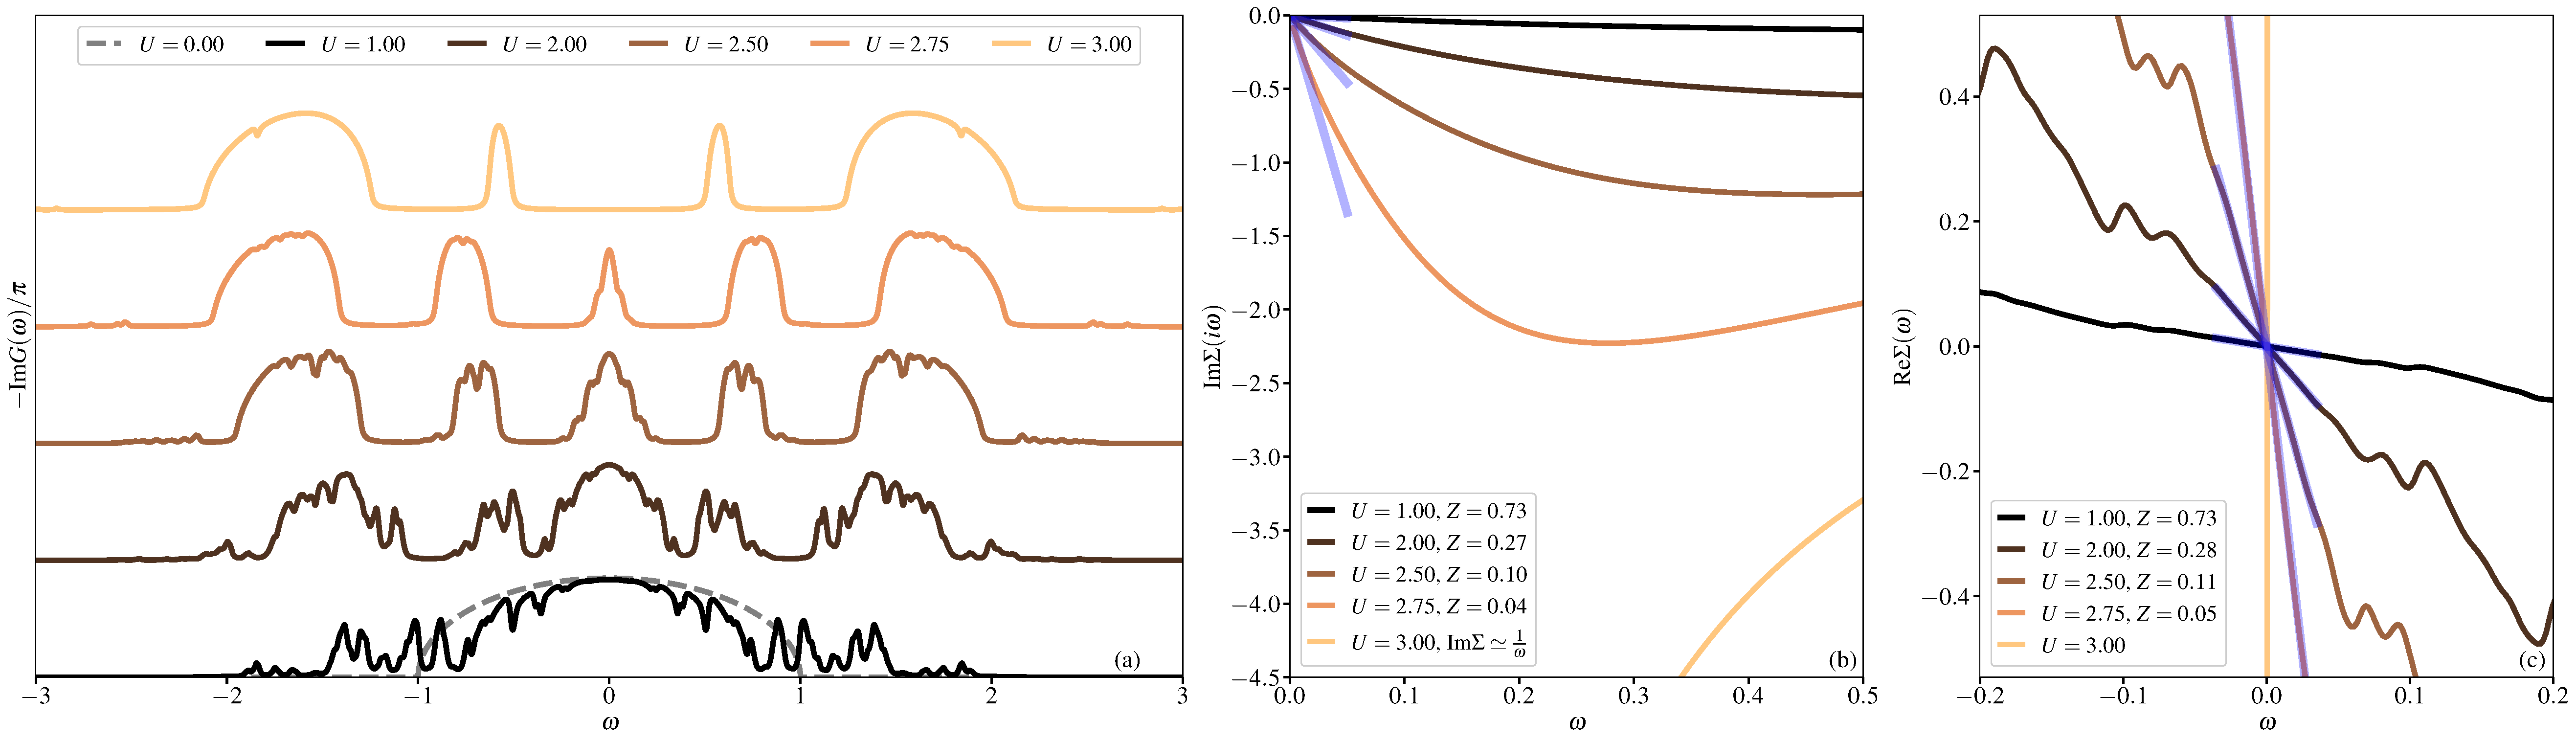
\includegraphics[width=\linewidth]{figures/figBethe.pdf}
    \caption{\label{figEx1}%
      \textbf{The metal-insulator Mott transition.}
      (a) Evolution of the spectral function $-\Im{G}(\omega)/\pi$ as
      a function of increasing interaction $U$. The critical
      interaction $U_\mathrm{c}\simeq 2.8D$ separates the correlated metal $U<U_\mathrm{c}$ from
      the Mott insulator $U>U_\mathrm{c}$.
      (b)-(c) The corresponding evolution of the Matsubara self-energy
      $\Im\Sigma(i\omega)$ (b) and
      real-axis one $\Re\Sigma(\omega)$ across the Mott
      transition. For a particle-hole symmetric case, both allow to
      estimate the renormalization constant $Z$ (see main text), using
      linear order expansion in frequency (blue solid lines). The
      values of $Z$ are reported in the legend.
      The Mott insulating solution is associated with a singularity at
      $\omega=0$ of $\Im\Sigma$.
    }
\end{figure}

The formation of a spectral gap separating the Hubbard bands in the 
Mott insulating phase is associated with the divergence of the 
imaginary part of the self-energy at the Fermi level. This divergence 
reflects the complete localization of the electrons, effectively 
suppressing coherent quasi-particle excitations. Causality dictates that the real part of the self-energy must also 
grow significantly near the singularity, making it impossible to 
satisfy the quasi-particle pole equation
$$
\omega+\mu-h^0-\e-\Re{\Sigma}(\omega)=0,
$$
which governs the formation of coherent excitations near the Fermi 
level.
Panels (B) and (C) illustrate this phenomenon by showing the evolution of the self-energy $\Sigma$. In panel (B), we present the Matsubara self-energy ${\rm Im}\Sigma(i\omega)$ in the low-energy regime. As the  interaction strength $U$ increases, this function progressively grows, eventually diverging as the critical interaction threshold $U > U_\mathrm{c}$ is crossed.
This divergence along the Matsubara axis is directly linked to the
particle-hole symmetry of the Bethe lattice, which pins the  ${\rm
  Im}\Sigma$ singularity at $\omega = 0$.
Panel (C) complements this picture by displaying the real part 
$\Re{\Sigma}(\omega)$ on the real-axis near the Fermi level. Here, increasing $U$ leads to a rapid rise of this component, culminating in a discontinuous behavior as the critical point is approached. This 
discontinuity directly reflects the divergence in the imaginary part
on the real-axis, confirming the transition to the Mott insulating state.


A quantitative measure of this transition is provided by the 
quasi-particle renormalization factor $Z$, which can be used to capture the degree of electron delocalization. This parameter ranges from 1 for a non-interacting metal to 0 for a fully localized Mott insulator. It is 
defined through the low-energy expansion of the self-energy as
$$
Z=\left(1-\frac{\partial\Re\Sigma}{\partial\omega}\Biggr|_{\omega\rightarrow
    0}\right)^{-1},
$$
which can also be estimated from the linear behavior of ${\rm Im}\Sigma(i\omega)$ for 
$\omega\to0$ in the metallic regime using the relation:
$$
   \frac{\Im\Sigma(i\omega_n)}{\omega_n}\Biggr|_{\omega_n\rightarrow 0}=
   \frac{1}{\pi}\int_{\mathbb R}d\epsilon \frac{\Re\Sigma(\epsilon)}{\epsilon^2}=
   \frac{\partial\Re\Sigma}{\partial\omega}\Biggr|_{\omega\rightarrow 0}.
$$

The linear fits highlighted in panels (B) and (C), along with the 
corresponding $Z$ values provided in the legends, clearly indicate that 
the slope of the self-energy at low energy increases with $U$ on both 
the Matsubara and real axes. At the transition point, this slope 
diverges, reflecting the onset of complete electron localization as 
$Z \to 0$, consistent with the singular behavior  
$-{\rm Im}\Sigma(\omega\to0) \to\infty$.






\subsubsection{Finite temperature (w2dynamics interface, CT-HYB benchmark)}\label{SecExamplesBetheDMFTW2D}
To demonstrate how the w2dynamics interface integrates with  \NAME, we briefly discuss how to solve the same problem, i.e. the Hubbard model on the Bethe lattice within DMFT using w2dynamics. 
In order to showcase the capabilities of \NAME to address low-temperature problems, we compare the continuous-time Quantum Monte Carlo (CTQMC) solver using the hybridization expansion method (CT-HYB) included in w2dynamics against the \NAME solver at finite temperature.  

Unlike \NAME, which provides only the impurity solver and bath optimization procedures and requires the user to implement the DMFT algorithm themselves (potentially using various methods), w2dynamics adopts a fundamentally different approach: a single Python script, {\tt DMFT.py}, handles the entire DMFT calculation, leveraging dedicated classes that implement the generic self-consistency. The w2dynamics calculation is then entirely controlled by a model-dependent parameters file {\tt Parameters.in}, which contains a number of variable specifications including options to control the ED solver inherited from \NAME. Further information about the functioning of w2dynamics can be found in Ref. \cite{Wallerberger2019CPC}           

Another important difference concerns the initial point of the iterative DMFT solution algorithm: while \NAME starts from a given discrete bath, w2dynamics is initialized with a zero self-energy function or alternatively reads this quantity from a converged solution file. Thus, when using the \NAME interface in w2dynamics, the initial Weiss field is determined using self-consistency and  an initial discrete bath is obtained through the \NAME bath optimization procedure. 

The following is the w2dynamics configuration file used to solve the Bethe lattice problem at finite temperature: 
\begin{lstlisting}[style=mybash,language={},numbers=none,basicstyle={\scriptsize\ttfamily}]
[General]
DOS             = Bethe           # support for the Bethe lattice is built-in
half-bandwidth  = 1               # list of half-bandwidths per orbital
NAt             = 1               # number of impurities
beta            = 100             # inverse temperature
mu              = 1.0             # chemical potential set to achieve half-filling
EPSN            = 0.0             # turns off filling-based chemical potential search
DMFTsteps       = 100             # given no convergence checking, we might want fewer
magnetism       = para            # symmetrize self-energies per spin
FileNamePrefix  = bethe_dmft_U2   # prefix for the output file name
fileold         = bethe_dmft*hdf5 # file to read an initial self-energy from
readold         = 0               # iteration number to read initial self-energy from, 0 turns off
mixing          = 0.5             # mixing, but mixes self-energies and not Weiss fields
mixing_strategy = linear          # linear mixing as in the Fortran example
FTType          = none            # (for CT-HYB): use the NFFT-measured G
solver          = EDIPACK         # use EDIpack as impurity solver, not default CTHYB

[Atoms]
[[1]]                             # one subsection per impurity
Nd              = 1               # number of orbitals
Hamiltonian     = Kanamori        # create a Hubbard-Kanamori interaction Hamiltonian
Udd             = 2.0             # equivalent to ULOC
Vdd             = 1.0             # equivalent to UST, meaningless for 1 orbital
Jdd             = 0.5             # equivalent to JH, JX and JP, also meaningless here

[EDIPACK]                         # further ED parameters, as in the Fortran example
NBATH           = 7               # number of bath sites
ED_TWIN         = True            # use twin symmetry
LFIT            = 2048            # number of Matsubara frequencies used for the bath fit
LANC_NGFITER    = 500             # number of Lanczos iterations for Green's function
CG_FTOL         = 1e-10           # conjugate-gradient tolerance
CG_NITER        = 2048            # maximum number of conjugate-gradient iterations
ED_FINITE_TEMP  = True            # at finite temperature T = 1/beta

[QMC]                             # Parameters for some grid sizes and the CT-HYB calculation
Ntau            = 1024            # imaginary time grid size
Niw             = 4096            # number of positive Matsubara frequencies
# parameters only relevant for CT-HYB follow
MeasGiw         = 1               # enable NFFT measurement of G
NCorr           = 175             # estimate of the autocorrelation length
Nmeas           = 200000          # number of measurements / sample size
Nwarmups        = 1000000         # number of initial warmup steps for Markov chain thermalization
\end{lstlisting}
Assuming the parameters are listed in a plain text file called 
{\tt bethe\_dmft.in}, the DMFT simulation can then by run on {\tt NC} cores via:
\begin{lstlisting}[style=mybash,numbers=none,morekeywords={mpiexec},deletekeywords={in}]
mpiexec -n NC /path/to/w2dynamics/DMFT.py bethe_dmft.in
\end{lstlisting}

The results are collected into an HDF5 \cite{The_HDF_Group_Hierarchical_Data_Format} archive in the usual w2dynamics format, including output quantities inherited from \NAME. Results can be viewed using the script {\tt hgrep} provided with w2dynamics or with other HDF5 tools. In this example we extract the Matsubara self-energy function $\Sigma(i\omega_n)$ for the last DMFT iteration:
\begin{lstlisting}[style=mybash,numbers=none]
/path/to/w2dynamics/hgrep latest siw-full -1
\end{lstlisting}

\begin{figure}%[t!]
  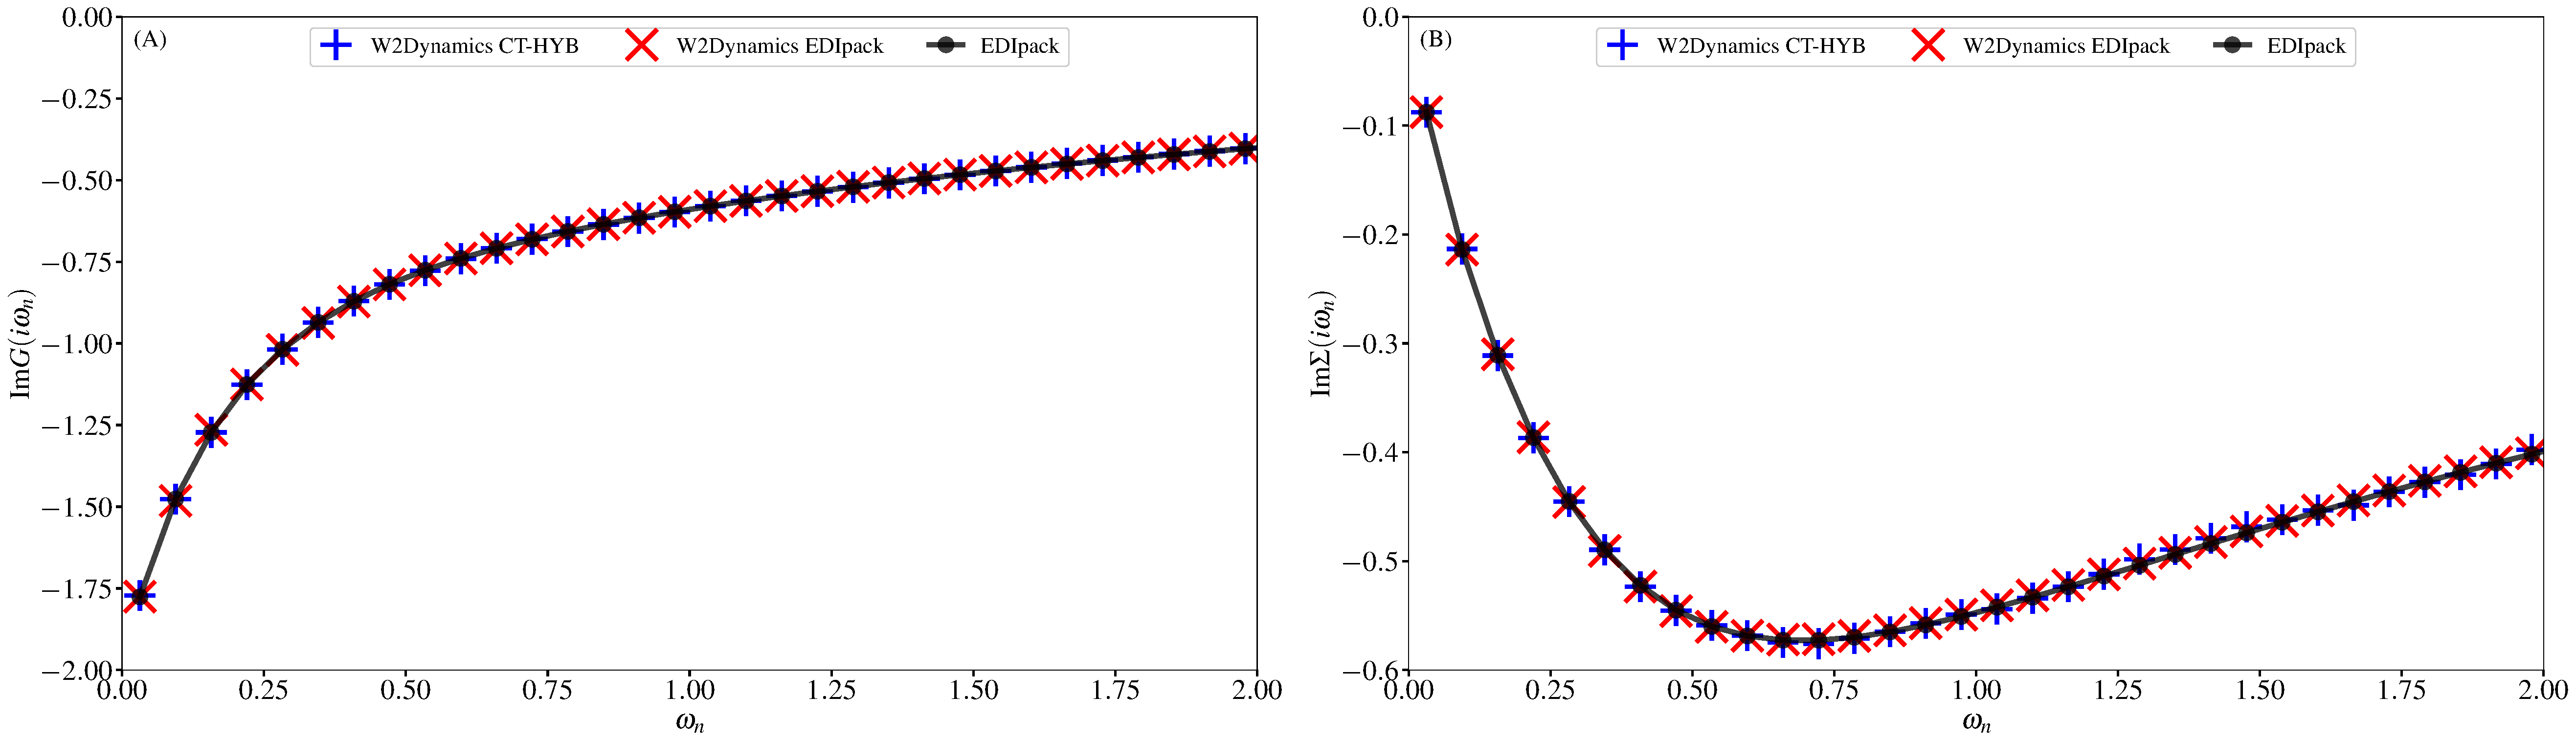
\includegraphics[width=\linewidth]{figures/figBetheW2D.pdf}
    \caption{\label{figEx1W}%
    \textbf{Finite temperature DMFT solution.}
    Comparison of the imaginary parts of the Green's function $\Im{G}(i\omega_n)$ and self-energy $\Im{\Sigma}(i\omega_n)$ from different solutions of the Hubbard model on the Bethe lattice using DMFT. Data are for $T/D=0.01$ and $U/D=2.0$. CTQMC results from the solver included with w2dynamics are compared against \NAME ED results, used both through the w2dynamics interface and with a standalone Fortran program. 
        }
\end{figure}

In \figu{figEx1W} we report a comparison of the results obtained using the hybridization expansion CTQMC and the \NAME ED method as solvers in w2dynamics. In addition we compare with results obtained using the Fortran API directly as shown in the previous subsection. Using DMFT, we solve the Hubbard model on a Bethe lattice for $T/D=0.01$ and $U/D=2.00$, corresponding to a correlated metallic state. 

In panel (A) we show the behavior of the imaginary part of the impurity Green's function $\Im{G}(i\omega_n)$ which is the direct output for both methods (note that w2dynamics does not directly have access to the real-axis Green's function when using the CTQMC solver). In panel (B) we show the same comparison for impurity self-energy $\Im{\Sigma}(i\omega_n)$. 
The results obtained from the three calculations are in excellent agreement with each other already for a small number of bath levels ({\tt NBATH=7}) and relatively low QMC statistics ({\tt Nmeas=200000} with {\tt NC=10} parallel processes).   



















\subsection{Attractive Hubbard model (Python API, {\tt ed\_mode=superc})}\label{SecExamplesAHM}
The second example we present concerns the DMFT description of the 
attractive Hubbard model \cite{Caffarel1994PRL,Toschi2005NJP,Toschi2005PRB} on a two-dimensional square lattice. 
This  example two main goals: (i) to demonstrate \NAME's support for $s$-wave superconductivity, and (ii) to showcase the Python API through a concrete example. 

The 
model Hamiltonian is given by:
$$
H = \sum_{\ka,\s} \epsilon(\ka) c^\dagger_{\ka\s} c_{\ka\s} 
    - U \sum_i n_{i\up} n_{i\dw},
$$
where $U > 0$, $c^\dagger_{i\s}$ 
is the creation operator for an electron at site $i$ with spin $\s$ and $c^\dagger_{\ka\s} = \tfrac{1}{\sqrt{N}} 
\sum_i e^{-i\ka \cdot R_i} c^\dagger_{i\s}$. 
The occupation operator is $n_{i\s} = c^\dagger_{i\s} c_{i\s}$, and 
the energy dispersion relation is $\e(\ka)=-2t[\cos{(k_x a)}+
\cos{(k_y a)}]$, where we set the lattice spacing 
$a=1$  and the choose the energy unit such that $4t=D=1$ for convenience.

The DMFT workflow for this case is largely similar to the previous 
example, but it now operates in the Nambu basis defined by the spinor $\psi_i=[\hat{c}_{i\up}\quad  \hat{c}^\dagger_{i\dw}]^T$ where the symbol $\hat{o}$ indicates the potential multi-orbital nature of the system, which reduces to a scalar in the present single-orbital case.
In this basis, the Green's function takes the matrix form:
\begin{equation}
  {\mathbf G} =
  \begin{pmatrix}
    \hat{G}_{\uparrow\uparrow} & \hat{F}_{\uparrow\downarrow}\\
    \hat{\bar{F}}_{\downarrow\uparrow}  &    \hat{\bar{G}}_{\downarrow\downarrow} \\
  \end{pmatrix}
\end{equation}
The components in the second row, denoted 
by $\hat{\bar{A}}$, are connected to the first row by particle-hole and time-reversal symmetries. The specific relations depend on the 
symmetry of the order parameter (here, $s$-wave) and whether the 
functions are defined on the Matsubara or real-frequency axis:
\begin{equation}
\begin{array}{cc}
  \hat{\bar{G}}(i\omega) = -\hat{G}^*(i\omega)\;; &  \hat{\bar{F}}(i\omega) = \hat{F}(i\omega)\\
  \hat{\bar{G}}(\omega)  = -\hat{G}^*(-\omega) \;; & \hat{\bar{F}}(\omega) = \hat{F}^*(i\omega)\\
\end{array}
\end{equation}  

The code implementation closely follows the structure of the previous 
example, with some notable adjustments related to the Nambu basis. 
These symmetries allow computing only the 
independent components in the first row, reducing 
the computational effort. 
Note that part of the operations required to implement the DMFT cycle are implemented in the Python module {\tt aux\_funx.py}, adapting from {\tt DMFTtools} functions.  
The initial part of the code handles the 
lattice structure and solver initialization, as described below.

\begin{lstlisting}[style=mypython,numbers=none,basicstyle={\scriptsize\ttfamily}]
import numpy as np
#Import EDIpack2py:
from edipack2py import global_env as ed
#Import MPI support 
import mpi4py
from mpi4py import MPI
#Import functions to build ${\color{comment-color}G_\mathrm{loc}}$ and perform DMFT self-consistency in Nambu space
from aux_funx import * 
import os,sys

#Start MPI framework:
comm = MPI.COMM_WORLD
rank = comm.Get_rank()
master = (rank==0)

#Functions: build 2D grid and dispersion ${\color{comment-color}\e(k)}$
def generate_kgrid(Nk):
    b1=2*np.pi*np.array([1.0,0.0])
    b2=2*np.pi*np.array([0.0,1.0])
    n1, n2 = np.meshgrid(np.arange(Nk), np.arange(Nk))
    n1=n1/Nk;n2=n2/Nk
    gridout = np.stack([n1.ravel(), n2.ravel()], axis=-1)
    return np.dot(gridout,[b1,b2])
    
def h_square2d(k,t):
  return -2*t*( np.cos(k[...,0,np.newaxis,np.newaxis])+
                np.cos(k[...,1,np.newaxis,np.newaxis]))*np.eye(ed.Norb)
    
#Read input
ed.read_input("inputAHM.conf")

#Generate ${\color{comment-color}H_k=\e(k)}$ and set Hloc
kgrid   = generate_kgrid(Nk)
Hk      = h_square2d(kgrid,t_hop)
Hloc    = np.sum(Hk,axis=0)/Nk**2
ed.set_hloc(Hloc.astype(complex))

#Build dispersion in Nambu space ${\color{comment-color}\e(k)\tau^z}$
HkNambu = np.array([h_square2d(kgrid,t_hop),-np.conj(h_square2d(-kgrid,t_hop))])

#Setup ED Solver
Nb=ed.get_bath_dimension()
bath = ed.init_solver()
\end{lstlisting}



The iterative scheme for the solution of DMFT closely follows the
sequence already discussed in \secu{SecExamplesBetheDMFT}:   
\begin{itemize}
\item[{\tiny {\bf EDIpack}}] Call the exact diagonalization {\bf impurity solver} {\tt
    ed.solve} providing the set of bath parameters $\vec{x}=\{V,h\}$  as input. 

\item Use the dedicated
  input/output \NAME procedures to retrieve the self-energy functions  
  $\hat{\Sigma}(i\omega)$ and $\hat{S}(i\omega)$ on the 
  Matsubara axis.
  
\item[{\tiny {\bf EDIpack}}]
  Evaluate the interacting local Green's functions $\hat{G}_\mathrm{loc}$ and
  $\hat{F}_\mathrm{loc}$:
  \begin{equation}
  {\mathbf G}_\mathrm{loc}(i\omega) =
  \int_\RRR d\e \rho(\e)
  \begin{pmatrix}
    (i\omega +\mu)\hat{\11} - \hat{h}^0 - \hat{\Sigma}(i\omega) -\e & -\hat{S}(i\omega) \\
    -\hat{S}(i\omega) & (i\omega +\mu)\hat{\11} + \hat{h}^0 +
    \hat{\Sigma}^*(i\omega) +\e\\
  \end{pmatrix}^{-1}
\end{equation}

\item[{\tiny {\it User}}] Update the Weiss field's components, respectively 
  $\GG_0^{-1}$ and $\FF_0^{-1}$, through the {\bf self-con\-sis\-ten\-cy}
  relation: $\mathbfcal{G}^{-1}_0(i\omega) = {\mathbf G}^{-1}_\mathrm{loc}(i\omega) +
  {\mathbf \Sigma}(i\omega)$ in Nambu space.
  
\item[{\tiny {\it User}}\textgreater\ {\tiny {\bf EDIpack}}] Optimize the bath parameters $\vec{x}$ to best describe the updated
    Weiss fields, potentially using the \NAME provided conjugate gradient  fit
    procedures.
  \end{itemize}
%
The corresponding implementation in Python reads:
\begin{lstlisting}[style=mypython,numbers=none,basicstyle={\scriptsize\ttfamily}]
#DMFT CYCLE
converged=False;iloop=0
while (not converged and iloop<ed.Nloop):
    iloop=iloop+1
    #Solve quantum impurity problem for the current bath
    ed.solve(bath)    

    #Retrieve the Matsubara self-energy components ${\color{comment-color}\Sigma(i\omega_n) }$ and ${\color{comment-color}S(i\omega_n) }$
    Smats = np.array([ed.get_sigma(axis="m",typ="n"),ed.get_sigma(axis="m",typ="a")])   
    
    #Perform self-consistency levaraging {\tt aux\_funx.py} procedures:
    Gmats = get_gloc(wm*1j,ed.xmu,HkNambu,Smats,axis="m")
    Weiss = dmft_weiss_field(Gmats,Smats)    
    
    #Fit Weiss field and update the bath
    bath = ed.chi2_fitgf(Weiss[0],Weiss[1],bath)

    #Error check
    err,converged=ed.check_convergence(Weiss,ed.dmft_error)
ed.finalize_solver()
\end{lstlisting}


\begin{figure}[t!]
  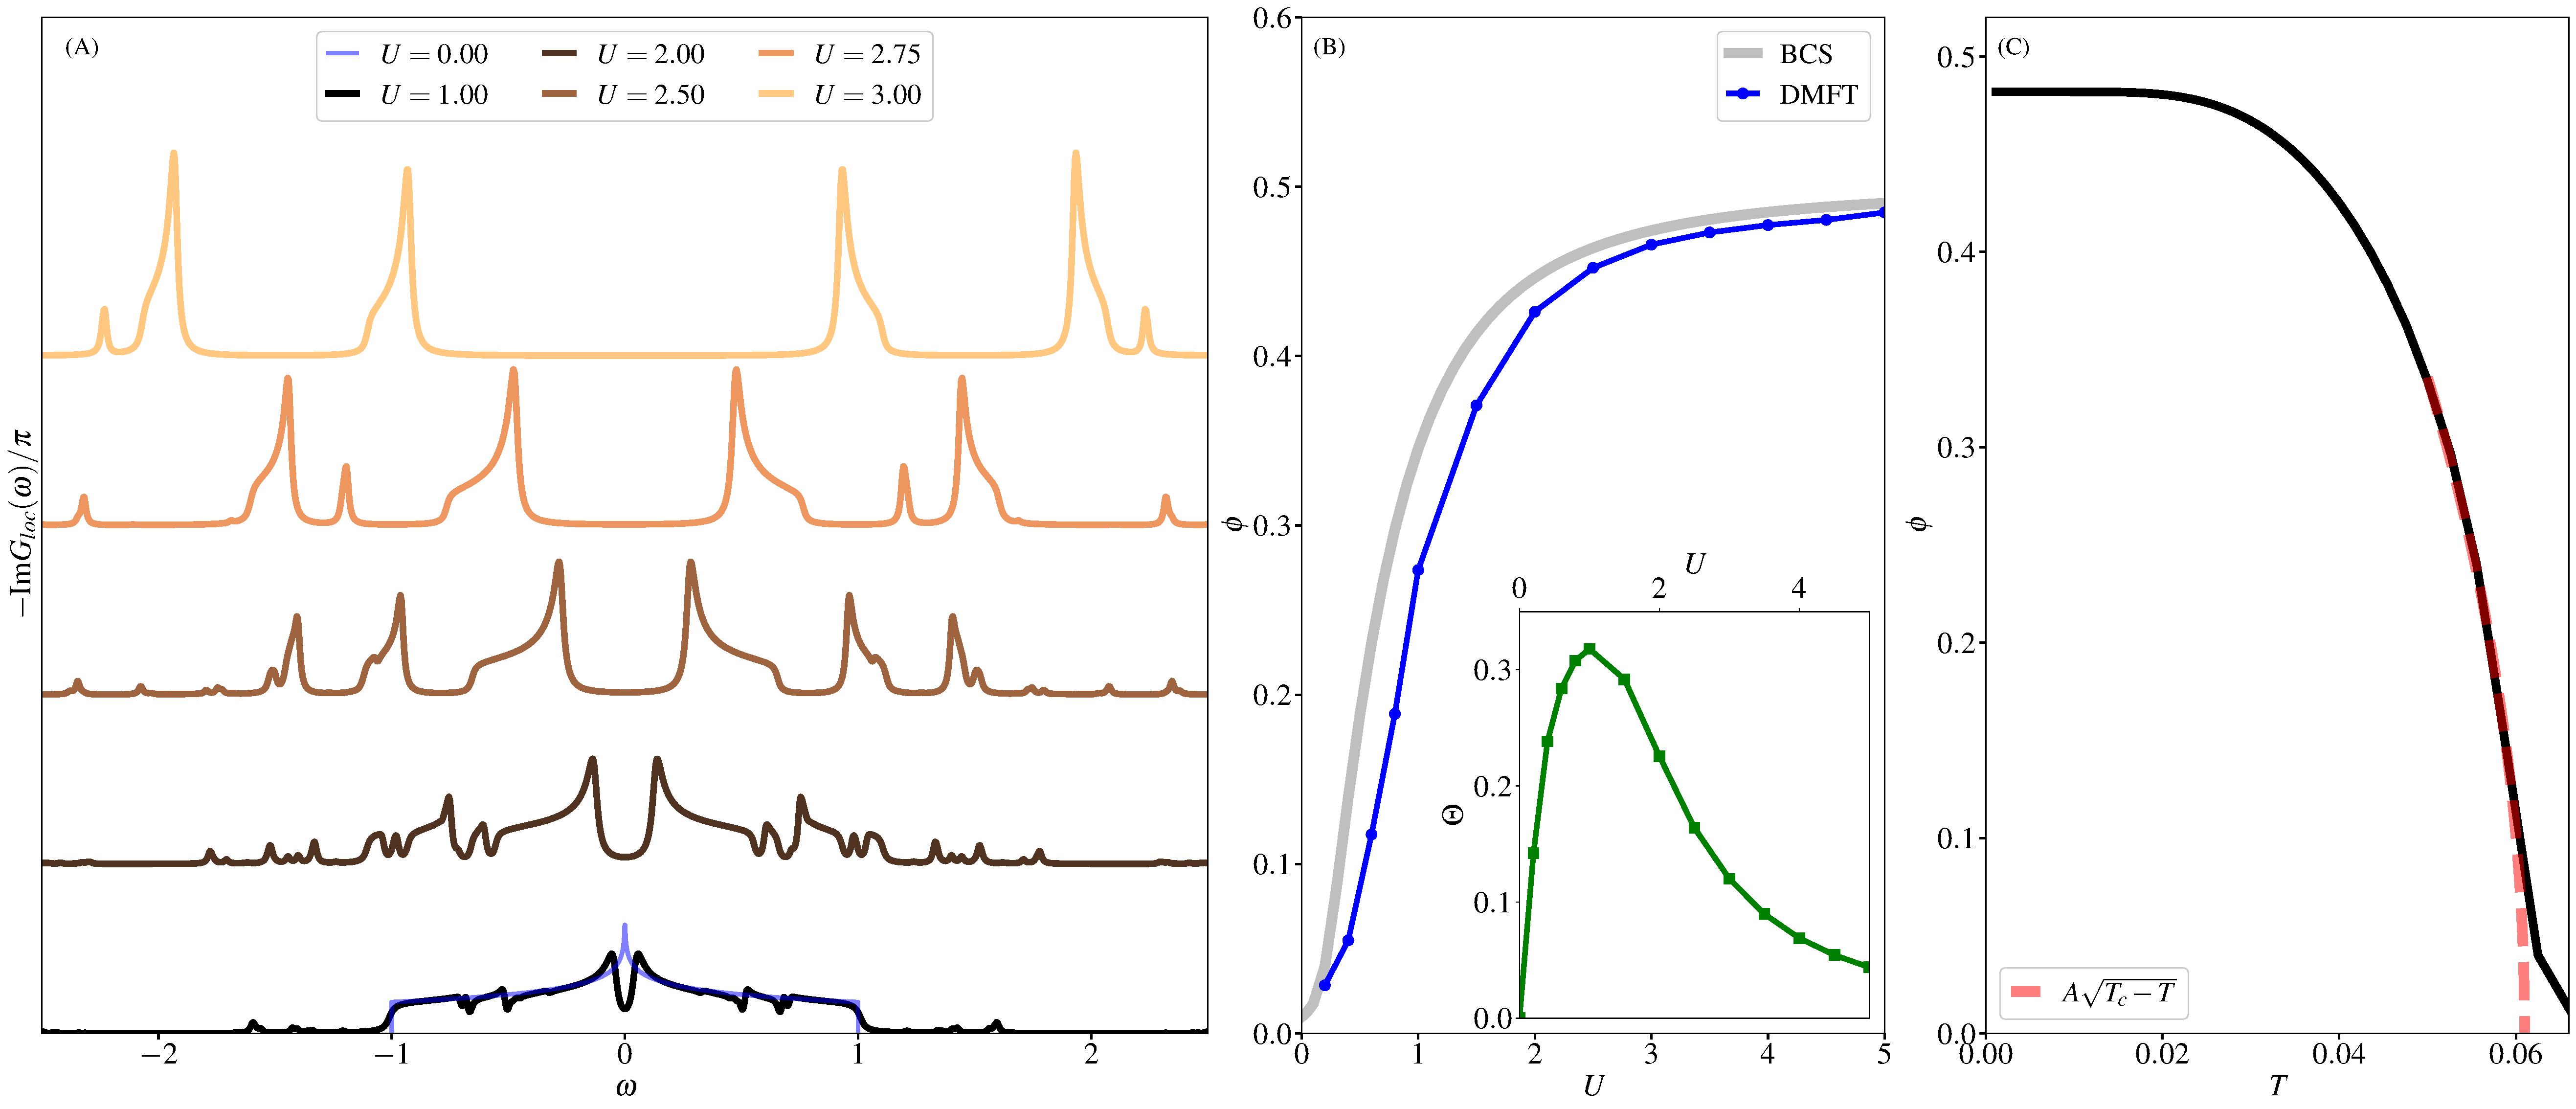
\includegraphics[width=\linewidth]{figures/figAHM.pdf}
    \caption{\label{figEx2}%
      \textbf{The BCS to BEC crossover.}
      (A) Evolution of the spectral functions
      $-\Im{G_\mathrm{loc}(\omega)}/\pi$ as a function of increasing
      attraction $U$. 
      (B) The order parameter $\phi=\langle c_\up c_\dw\rangle$ as a
      function of the attraction $U$. Data for BCS (gray) is compared
      to DMFT results (blue line and symbols). Inset: the correlation strength
      $\Theta$ (see main text) as a function of the
      attraction $U$ across the BCS-BEC crossover. 
      (C) Superconducting order
      parameter $\phi$ as a function of temperature across the
      superconductor-to-normal phase transition. Data for $U=4$. The
      fit highlights the critical behavior with a mean-field exponent
      $\beta=1/2$ (red dashed line) and parameters $A\simeq 3.7$, $T_\mathrm{c}=0.61$.       
        }
\end{figure}

\paragraph{Results.}
Here we showcase some results for the DMFT solution of the 
attractive Hubbard model across the BCS-to-BEC crossover regime \cite{Toschi2005PRB,Toschi2005NJP,Amaricci2014PRA} 
illustrating the capability of \NAME to handle $s$-wave 
superconductivity at both zero and finite temperatures.

To begin, panel (A) of \figu{figEx2} shows the evolution of the 
spectral density, obtained from the local normal Green's function as 
$-\tfrac{1}{\pi}\Im G_\mathrm{loc}(\omega)$, as a function of the 
attraction $U$. For any finite $U$, the Van Hove peak near the Fermi level characteristic of the 2D square lattice (visible at 
$U = 0$) is split by the formation of a superconducting gap. The latter reflects the emergence of a finite 
order parameter $\phi = \langle c_\up c_\dw \rangle$ and onset of superconducting coherence.

The evolution of the order parameter with attraction $U$ is presented in panel (B). The figure  
highlights the crossover from the weak-coupling BCS regime to the 
strong-coupling BEC regime. In the BCS limit, $\phi$ displays the 
characteristic exponential growth with $U$, known to be 
computationally challenging. In the opposite, strong-coupling, limit 
$\phi$ saturates at its theoretical maximum of $\phi \rightarrow 1/2$. The comparison with the BCS mean-field result 
(gray line) reveals the effect of local dynamical fluctuations, which  slightly suppress the order parameter, particularly in the intermediate regime. 
To further quantify these dynamical effects, we plot in the inset of the same panel the 
{\it correlation strength} \cite{Amaricci2015PRL,Amaricci2016PRB}
$\Theta=|S(i\omega\to 0)-S(i\omega\to\infty)|/S(i\omega\to\infty)$. 
Large values of $\Theta$ indicate an anomalous self-energy with 
significant dynamical effects, hence a more correlated superconducting state.
Our results show that the DMFT solution significantly departs from the BCS picture in the strongly correlated intermediate-coupling, a regime known to host the highest critical temperature \cite{Toschi2005NJP,Toschi2005PRB}.
% A different angle further illustrating the impact of dynamical fluctuations, is reported in panel (D). We show the evolution of the double occupancy $d = \langle n_\up n_\dw \rangle$ as a function of $U$ compared to the MF expression $d = 1/4 + \phi^2$. The DMFT 
% results obtained with \NAME show a slight increase in $d$ over the MF prediction in the BCS regime. As $U$ increases and local correlation becomes sizable, the double occupancy drops below 
% the MF result. 

Finally, we demonstrate the capability of \NAME to describe finite 
temperature effects. Panel (E) shows the temperature dependence of 
the order parameter $\phi(T)$ across the superconducting-to-normal 
transition. The mean-field nature of this transition is evident from 
the scaling near the critical temperature 
$\phi \sim (T_\mathrm{c} - T)^\beta$ with $\beta = 1/2$, consistent 
with  Ginzburg-Landau theory.

These results collectively illustrate the versatility of \NAME in 
handling both ground state and finite temperature superconducting 
phases, for instance capturing the complex physics of the BCS-BEC crossover with high accuracy.







\begin{figure}[ht!]
    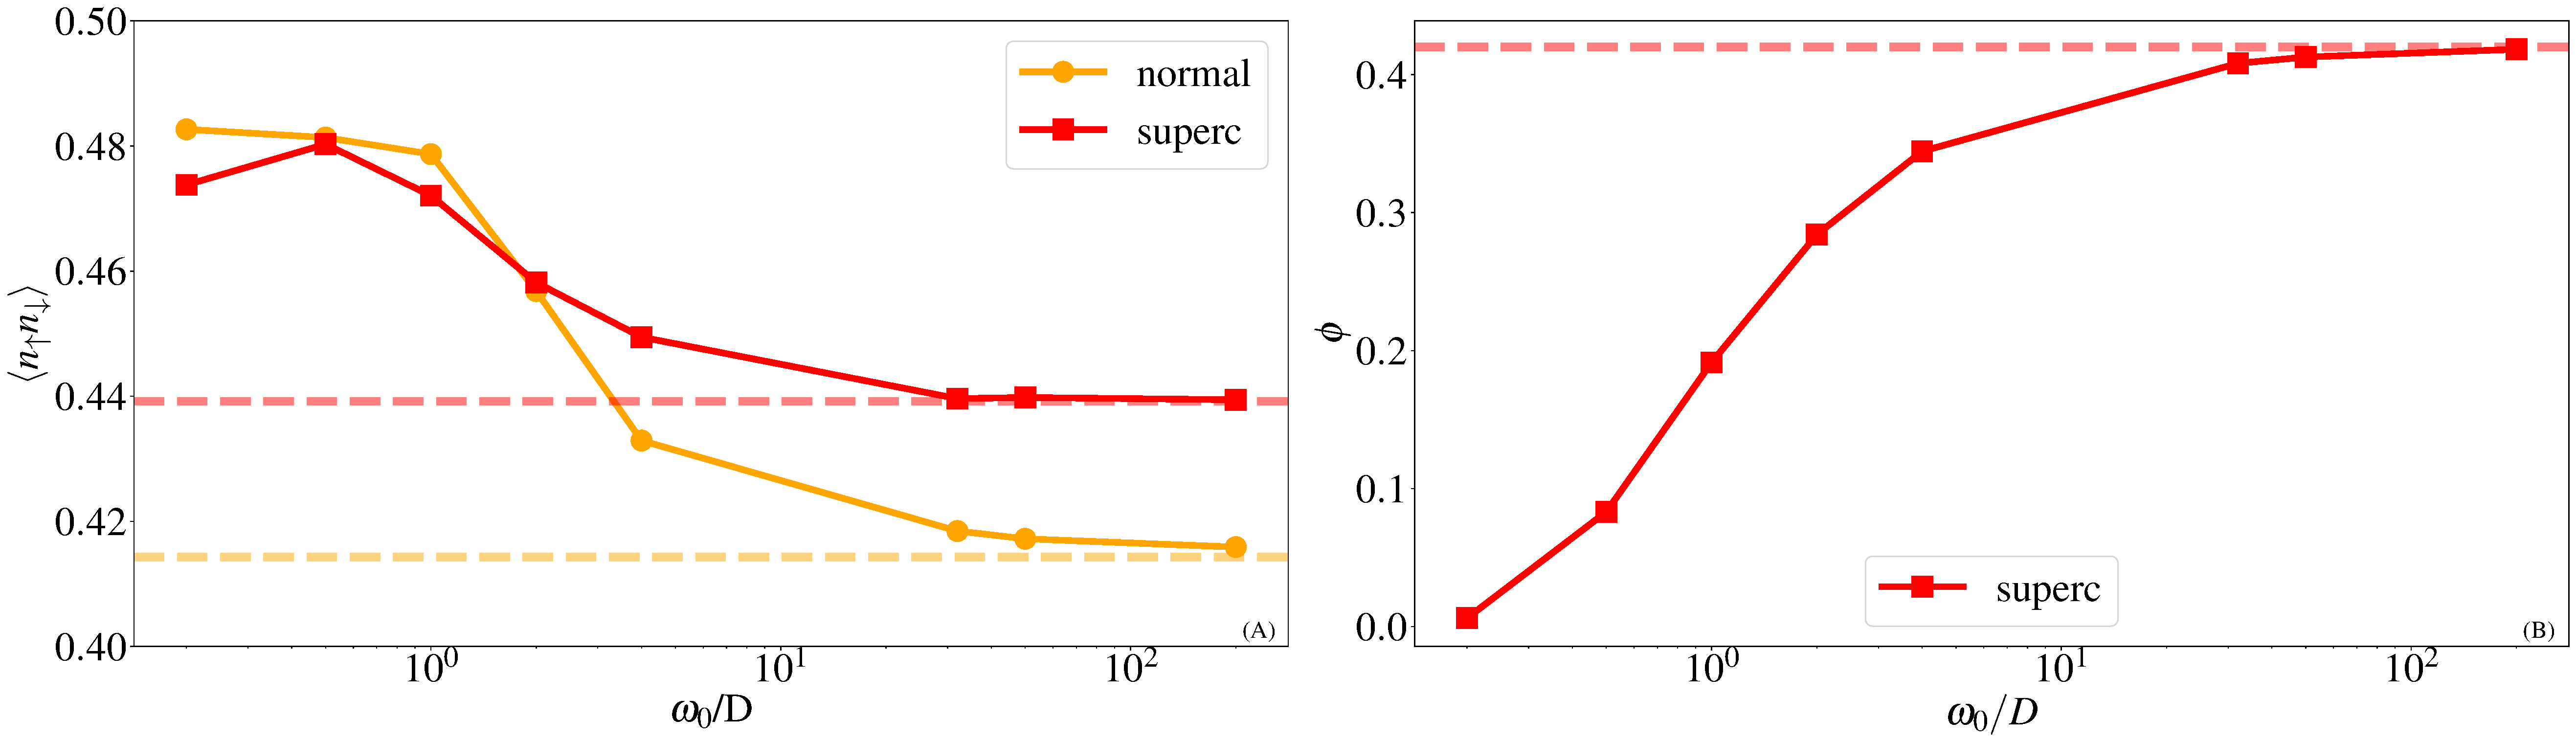
\includegraphics[width=\linewidth]{figures/figBethe_Holstein.pdf}
    \caption{\label{figEx5}
      Evolution of the double occupancy (A) and superconductive order parameter (B) as a function of $\omega_0/D$ for $\lambda=1$ in the normal (orange) and superconductive (red) phase. The horizontal broken lines are the values for the corresponding Hubbard model in the anti-adiabatic limit.}
\end{figure}


\subsection{Holstein model on the Bethe lattice (electron-phonon coupling)}

One of the new features introduced in \NAME is the support for local phonons in combination with superconductivity,
i.e. {\tt ed\_mode=superc}. In order to illustrate this property using a simple application, in this example we discuss the normal and
superconductive solution of the pure Holstein model on the Bethe lattice within DMFT.
Note that the code
implementation for this case is essentially identical to the listings in the previous sections
\ref{SecExamplesBetheDMFT} ({\tt ed\_mode=normal}) and
\ref{SecExamplesAHM} ({\tt ed\_mode=superc}), provided electron-electron interaction is set to zero and phonon parameters are properly configured.  

We consider the model introduced in \secu{SecExamplesBetheDMFT}
with $U=0$ and the additional phononic and electron-phonon terms:
\begin{equation} \label{eqex:H_Holstein}
    H_\mathrm{int} = \sum_i \Big[\omega_0 b^\dagger_i b_i + g(b^\dagger_i +
    b_i)\sum_{\sigma}\left(c^\dagger_{i\sigma}c_{i\sigma}
    -\frac{1}{2}\right)\Big]. 
\end{equation}
We focus on the half-filling regime of the particle-hole symmetric Bethe lattice DOS. We set the half-bandwidth as our energy unit $D=1$ and introduced the electron-phonon coupling $\lambda = \tfrac{2g^2}{\omega_0}$.  
The iterative DMFT solution algorithm follows the same principles illustrated in the previous sections. 

\paragraph{Results.}
In the following we discuss the adiabatic ($\omega_0\to0$) to
anti-adiabatic ($\omega_0\to\infty$) crossover for
the uniform solution of the Holstein model at constant coupling $\lambda=1.0$.
%
In the anti-adiabatic limit, the Holstein interaction takes a
particularly simple form:
\begin{equation}\label{HlikeAttraction}
    H_\mathrm{int} \overset{ \omega_0 \rightarrow \infty}{ \longrightarrow } -\frac{\lambda}{2} \sum_i \Big[\sum_\sigma\left(c^\dagger_{i\sigma}c_{i\sigma} -\frac{1}{2}\right) \Big]^2,
\end{equation}
which describes a local Hubbard-like attraction among electrons
(mediated by local phonons).
In the  adiabatic limit, $\omega_0 \rightarrow 0$ the system
enters a Bipolaronic Insulating phase for our
choice of the coupling \cite{Capone2006PRB}. 


We characterize the model solution by showing the evolution of the
double occupation $\langle n_{\up}n_{\dw}\rangle$ as a function of the
phonon frequency $\omega_0$, see panel (A) of \figu{figEx5}. In this panel we compare
the behavior for the normal phase ({\tt ed\_mode=normal}) and the superconductive
phase ({\tt ed\_mode=superc}). Our results capture the whole
crossover from adiabatic to anti-adiabatic regime. In the former
regime, the double occupation takes a similar value for the two
phases. However, approaching the anti-adiabatic regime, the two
solutions reach the limiting values corresponding to the residual
attraction \equ{HlikeAttraction}.   
To better characterize the nature of the superconducting
phase in the Holstein model, we report the evolution of the anomalous order
parameter $\phi$ in the adiabatic to anti-adiabatic crossover, see panel (B) of \figu{figEx5}.
The DMFT results obtained with \NAME show a rapid increase in the
superconducting order parameter as phonon frequency grows
large. Finally, in the anti-adiabatic regime, $\phi$ saturates to a
finite value corresponding to the attractive Hubbard-like interaction
of strength $\lambda/2$. 









\begin{figure}[t!]
    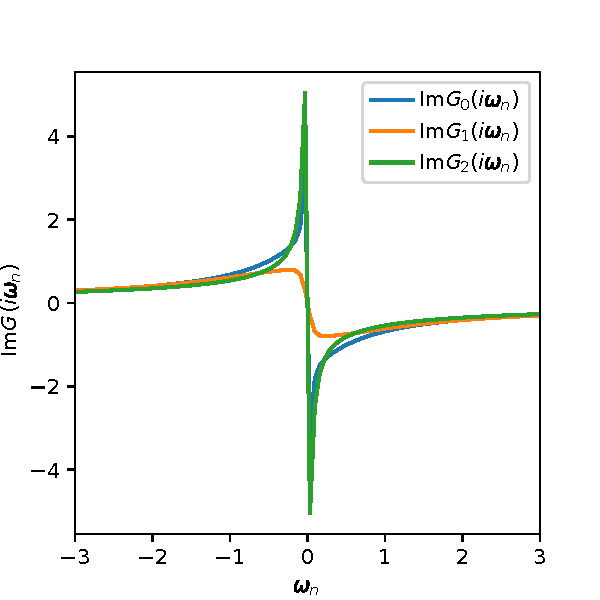
\includegraphics[width=0.5\linewidth]
        {figures/G_iw.pdf}
    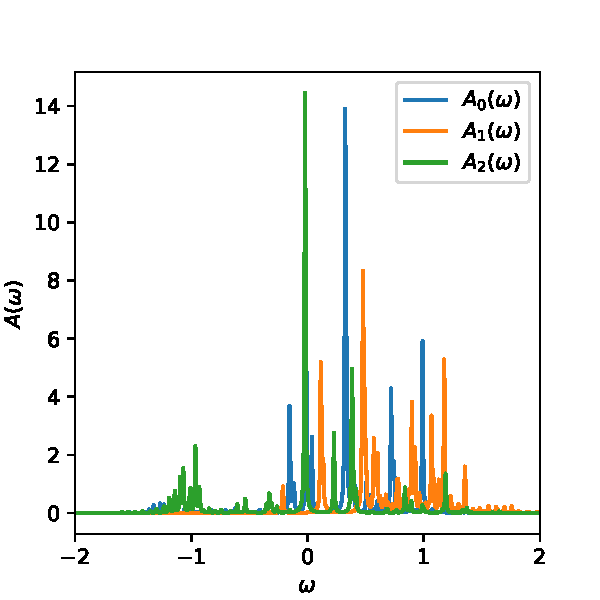
\includegraphics[width=0.5\linewidth]
        {figures/A_w.pdf}
    \caption{\label{figEx3}%
        Imaginary part of the Matsubara Green's function $G_\alpha(i\omega_n)$ (left) and the
        corresponding orbital-resolved spectral function $A_\alpha(\omega) = -\Im{G_\alpha(\omega)} / \pi$ (right) computed for a
        three-orbital impurity model with an interaction of the Hubbard-Kanamori
        type (\ref{Hint}). This illustration is produced by the EDIpack2TRIQS
        example script presented in \secu{SecExamplesTRIQS}.
    }
\end{figure}

\subsection{Multi-orbital impurity with Kanamori
  interaction (TRIQS interface)}
\label{SecExamplesTRIQS}

We proceed to demonstrate how to use the EDIpack2TRIQS compatibility
layer (\secu{sSecInteropTRIQS}) to solve a quantum system comprised by a
3-orbital correlated impurity coupled to a few non-interacting bath sites.
The interaction term of the impurity Hamiltonian is in the Hubbard-Kanamori
form of \equ{Hint}.

A Python script implementing a calculation that makes use of EDIpack2TRIQS
generally begins with a few module imports.
\lstinputlisting[style=mypython,
                 numbers=none,
                 basicstyle={\scriptsize\ttfamily},
                 firstline=1, lastline=13]
{figures/hubbard_kanamori.py}

One then proceeds to defining the system under consideration. In this case we
consider an impurity atom with three correlated orbitals and two bath states
per each impurity orbital, which corresponds to {\tt bath\_type=normal} in \NAME. This information must be encoded in the fundamental
set objects that are later used to construct the solver.
\lstinputlisting[style=mypython,
                 numbers=none,
                 basicstyle={\scriptsize\ttfamily},
                 firstline=15, lastline=26]
{figures/hubbard_kanamori.py}
The next step is to define a TRIQS many-body operator expression that represents
the Hamiltonian to be diagonalized.
\lstinputlisting[style=mypython,
                 numbers=none,
                 basicstyle={\scriptsize\ttfamily},
                 firstline=28, lastline=67]
{figures/hubbard_kanamori.py}
Finally, one creates a solver object and performs the actual calculation by
calling its method {\tt solve()}. This is normally the most time- and
memory-consuming step.
\lstinputlisting[style=mypython,
                 numbers=none,
                 basicstyle={\scriptsize\ttfamily},
                 firstline=69, lastline=83]
{figures/hubbard_kanamori.py}
The computation results are readily available as attributes of the solver
object. The following code snippet shows how to access measured expectation
values of the static observables, and how to employ the plotting framework of
TRIQS to visualize the obtained Matsubara and real-frequency impurity Green's
functions (\figu{figEx3}).
\lstinputlisting[style=mypython,
                 mathescape=false,
                 numbers=none,
                 basicstyle={\scriptsize\ttfamily},
                 firstline=85, lastline=113]
{figures/hubbard_kanamori.py}


















\subsection{Interacting Bernevig-Hughes-Zhang model (Fortran API, {\tt ed\_mode=nonsu2})}
In this section, we focus on the DMFT solution of the interacting
Bernevig-Hughes-Zhang (BHZ) model.
As shown in Ref. \cite{Amaricci2023PRB}, this model exhibits an excitonic phase at moderate
interactions in which opposite orbital electrons and holes across the band gap bind and form a coherent phase \cite{Knolle2017PRL,Jia2020,Varsano2020NN,Blason2020PRB,Amaricci2023PRB,Giuli2023PRB}

We consider a system of two-orbital electrons on a square
lattice, interacting via a Hubbard-Kanamori term. This system realizes a quantum spin Hall insulator \cite{Kane2005PRL,Bernevig2006S,Hasan2010RMP,Hohenadler2011PRL,Amaricci2015PRL,Tang2017NP,Amaricci2023PRB,Paoletti2024PRB}.
We consider a suitable matrix basis in terms of the Dirac
matrices $\Gamma_{a\a}=\sigma_a\otimes \tau_\a$, where $\sigma_a$ and
$\tau_\a$ are Pauli matrices, respectively, in the spin and orbital
pseudo-spin space. The  model Hamiltonian reads
$$
H = \sum_{k}\psi_{k}^\dagger H(k)\psi_{k} + H_{\rm int},
$$
where $\psi_{k}=[c_{1\uparrow k}, c_{2\uparrow k},
c_{1\downarrow k}, c_{2\downarrow k} ]^T$ is the spinor collecting
annihilation operator $c_{a\sigma k}$ destroying an electron at
orbital $a=1,2$ with spin  $\sigma=\up,\dw$ and lattice momentum
$k$. The non-interacting part of the Hamiltonian is:
$$
H(k) = \left[M-2t(\cos{k_x}+\cos{k_y}) \right]\Gamma_{03} +
   \lambda\sin{k_x}\Gamma_{31} -   \lambda\sin{k_y}\Gamma_{02},
$$
where $M$ is the mass term, which plays the role of a crystal
field splitting among the orbitals. The presence of this term breaks
the symmetry in the orbital pseudo-spin channel.
The  interaction reads: 
$$
   H_{\rm int} = (U-J)\frac{\hat{N}(\hat{N}-1)}{2} - J\left( \frac{1}{4}\hat{N}^2 +
   \hat{S_z}^2 - 2 \hat{T_z}^2\right),
 $$
 where $\hat{N}=\tfrac{1}{2}\psi_i^\dagger \Gamma_{00}\psi_i$ is the
total density operator,
$\hat{S_z}=\tfrac{1}{2}\psi_i^\dagger \Gamma_{30}\psi_i$ is the total
spin polarization operator and $\hat{T_z}=\tfrac{1}{2}\psi_i^\dagger
\Gamma_{03}\psi_i$ is the orbital pseudo-spin polarization operator.
This form corresponds to the density-density part of the
Kanamori interaction. We neglect the pair-hopping and spin-flip purely
for numerical reasons \cite{Amaricci2022CPC}. 
%
In the non-interacting regime this model describes a
quantum spin Hall insulator (QSHI) for $M<4t$ and a trivial Band
Insulator (BI) for $M>4t$.
The transition point at $M=4t$ describes the formation of a gapless Dirac state at  $k=[0,0]$.  


The code implementation follows the same guidelines discussed above for the other examples. The user is required to generate the Hamiltonian $H(k)$ on a discretized Brillouin zone. 
This is employed to evaluate the local interacting Green's function:
$$
G_\mathrm{loc}(z) = \tfrac{1}{N_k}\sum_k \left[z+\mu-H(k)-\Sigma(z)
\right]^{-1}, 
$$
entering in self-consistency conditions $\GG^{-1}=G_\mathrm{loc}^{-1}+\Sigma$. 
Here  $\z\in\CCC$, $N_k$ is the number of $k$-points   and $\Sigma(z)$ is the self-energy matrix  obtained from the DMFT solution of the problem.  
Moreover, the $H(k)$ is used to  construct the {\it renormalized} topological Hamiltonian \cite{Wang2010PRL,Wang2012PRX,Blason2023PRB}
$$
H_\mathrm{top} = \sqrt{Z}[H(k) + \Re\Sigma(\omega\to0)]\sqrt{Z}, 
$$
where $Z$ is the renormalization constant matrix. The matrix $H_\mathrm{top}$ describes the
low-energy properties of the many-body solution and can be used to characterize the topological nature of the interacting system \cite{Gurarie2011PRB,Wang2012PRX,Wagner2023NC,Blason2023PRB,Bau2024PRB}.  




\begin{figure}[t!]
  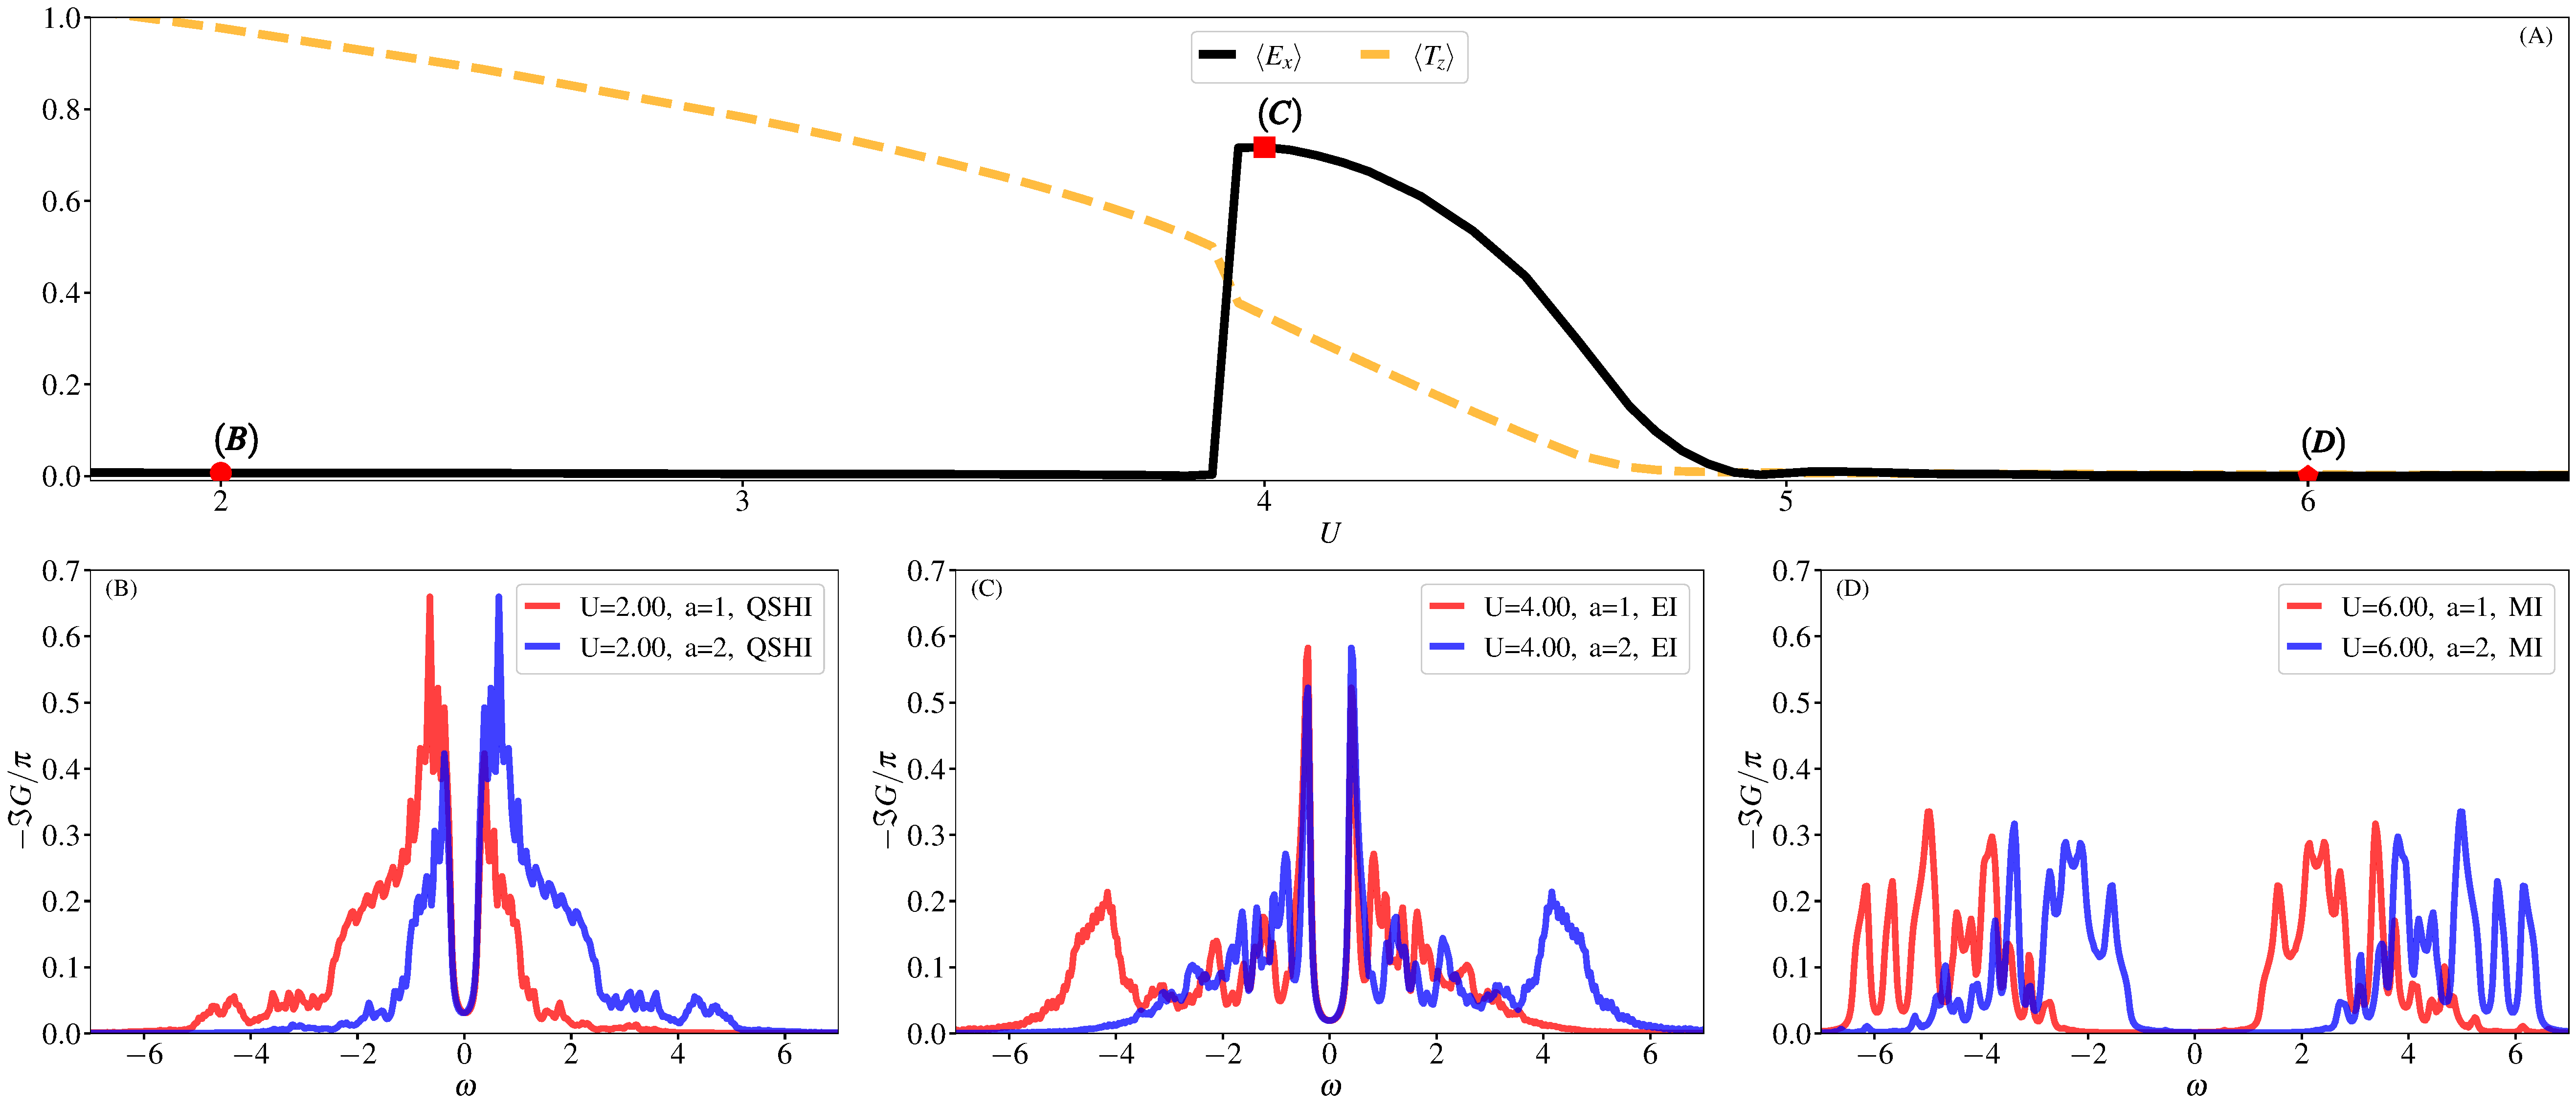
\includegraphics[width=\linewidth]{figures/figBHZ.pdf}
    \caption{\label{figEx4}%
      \textbf{Topological and Exciton Transition.}
      (A) Evolution of the spin-triplet,
      in-plane excitonic order parameter $\langle E_x\rangle$ (black solid line) and
      orbital polarization $\langle T_z\rangle$ (orange dashed line) as a function of the
      interaction $U$.
      (B-D) Spectral functions of the two orbital electrons for three
      values of the interaction $U=2.00$ (red circle), $4.00$ (red
      square) and $6.00$ (red diamond) capturing, respectively, the
      QSHI \textbf{\textit{(B)}}, the Excitonic Insulator \textbf{\textit{(C)}} and the Mott Insulator
      \textbf{\textit{(D)}}. 
    }
\end{figure}

\paragraph{Results}
To capture the possible symmetry breaking in any excitonic channel
driven by the local interaction, we consider the vector order
parameter
$\vec{E}=[E_0,E_x,E_y,E_z]$, where $E_a=\langle\psi^\dagger
\Gamma_{a1}\psi \rangle$ \cite{Budich2014PRL,Kunes2014PRB,Kaneko2015JOPCS,Kunes2015JOPCM,Knolle2017PRL,Guerci2019PRM,Geffroy2019PRL,Mazza2020PRL,De-Palo2023PRB}.

The first component $E_0$ describes the singlet excitonic state,
whereas the remaining ones correspond to the triplet states with
different spin orientation \cite{Blason2020PRB,Amaricci2023PRB}.   
The analysis of the strong-coupling regime as well as impurity
excitonic susceptibility available in \NAME suggest the possible
instability to an in-plane spin-triplet exciton phase, i.e. with $E_x$
and/or $E_y$ different from zero, see \cite{Amaricci2023PRB}.
Interestingly, this state breaks several symmetries including
time-reversal and spin SU(2), which protect the topological state.

Here we showcase the DMFT description of the excitonic phase in the interacting BHZ model as a way to
illustrate the \NAME ability to capture matter phases with lowered spin-symmetry ({\tt ed\_mode=nonsu2}) and the use of {\tt
  bath\_type=replica}.

The initial part of the code implementation is a simple generalization of the previously discussed cases. 
The next non-trivial steps are: i) construct the lattice Hamiltonian $H(k)$ and the corresponding local part $H_\mathrm{loc}$, which determines the impurity properties, and ii) construct a matrix basis representation for the replica bath. These two steps can be implemented as follows: 

\begin{lstlisting}[style=fstyle,numbers=none,basicstyle={\scriptsize\ttfamily}]
   !> Set $\smash{{\color{comment-color}H_\mathrm{loc}}}$ 
   allocate(Hloc(Nso,Nso))
   Hloc = sum(Hk,dim=3)/Lk
   where(abs(dreal(Hloc))<1d-6)Hloc=zero

   !EDIpack: set the impurity Hamiltonian: $\smash{{\color{comment-color}H_\mathrm{loc}\to h^0}}$
   call ed_set_hloc(Hloc)


   !EDIpack: set the replica bath matrix basis $\smash{{\color{comment-color}  \vec{\Gamma}}}$ and $\smash{{\color{comment-color}  \vec{\lambda}}}$
   !Here Nsym=4.
   !Build the basis and init the variational parameters:
   allocate(lambdasym_vector(Nbath,4))
   allocate(Hsym_basis(Nso,Nso,4))
   Hsym_basis(:,:,1)=Gamma03 ;lambdasym_vector(:,1)= Mh
   Hsym_basis(:,:,2)=Gamma01 ;lambdasym_vector(:,2)= sb_field
   Hsym_basis(:,:,3)=Gamma31 ;lambdasym_vector(:,3)= sb_field
   Hsym_basis(:,:,4)=Gamma11 ;lambdasym_vector(:,4)=-sb_field
   
   !EDIpack: set the basis and initial values of $\smash{{\color{comment-color}  \vec{\lambda}}}$
   call ed_set_Hreplica(Hsym_basis,lambdasym_vector)
   
   !EDIpack: get bath dimension and allocate user bath to this size
   Nb=ed_get_bath_dimension(4)
   allocate(Bath(Nb))
   
   !EDIpack: Initialize the ED solver
   call ed_init_solver(bath)
\end{lstlisting}
Here we use the local non-interacting Hamiltonian 
$H_\mathrm{loc}=\tfrac{1}{N_k}\sum_k H(k)$ to set 
$h^0_{\a\b\s\s'}$, i.e. the impurity Hamiltonian. To anticipate the
possibility of forming an excitonic ordered phase, the replica bath
is constructed out of a matrix basis with 4 distinct elements
$\Gamma_{03}$, $\Gamma_{01}$, $\Gamma_{31}$, $\Gamma_{11}$ which are proportional, respectively, to the mass term, the exciton singlet
$E_0$, the exciton triplet along easy-axis $E_z$ and in-plane
$E_x$ (we assume $E_y=0$ leveraging on residual $U(1)$ in-plane symmetry). 
In the following we consider the case of $M=1$, which corresponds to a QSHI in the non-interacting limit and $J/U=0.25$.
The implementation is nearly identical to the cases discussed above and
we report it here for completeness:
\begin{lstlisting}[style=fstyle,numbers=none,basicstyle={\scriptsize\ttfamily}]
   iloop=0;converged=.false.
   do while(.not.converged.AND.iloop<nloop)
     iloop=iloop+1
     
     !EDIpack: Solve the impurity problem
     call ed_solve(bath)

     !EDIpack: Retrieve ${\color{comment-color} \Sigma(i\omega)}$
     call ed_get_sigma(Smats,axis="mats")
     
     !Get $\color{comment-color}G_\mathrm{loc}$ using $\color{comment-color}\mathrm{DMFTtools}$
     call get_gloc(Hk,Gmats,Smats,axis="m")
     
     !Update the Weiss field (self-consistency) using $\color{comment-color}\mathrm{DMFTtools}$
     call dmft_self_consistency(Gmats,Smats,Weiss)

     !Linear mixing the Weiss fields
     if(iloop>1)Weiss = wmixing*Weiss + (1.d0-wmixing)*Weiss_;Weiss_=Weiss

     !EDIpack: Fit to update the bath
     call ed_chi2_fitgf(Weiss,bath,ispin=1)
     
     !Check convergence: using $\color{comment-color}\mathrm{DMFTtools}$
     converged = check_convergence(Weiss(1,1,:),dmft_error,nsuccess,nloop)
   enddo  
 \end{lstlisting}
 
%
The main effect of the interaction on the topological properties is contained in the mass term renormalization.  
The real part of the self-energy being proportional to $\Gamma_{03}$
corrects the mass term with respect to its bare value: $M_\mathrm{eff}=M+\tfrac{1}{4}\Tr{\Re\Sigma(i\omega\to0)}$. 
To leading order (mean-field) this correction is proportional to $\tfrac{U-5J}{4}\langle
\hat{T}_z\rangle$. So, for our choice of parameters, the effect of
interaction would be to effectively reduce the mass term. Thus, in the strong-coupling limit the two orbitals get populated by one electron per site, reaching the
conditions for the formation of a Mott insulating state.
This effect is highlighted in panel (A) of \figu{figEx4}, where we report the progressive reduction of the
orbital polarization  $\langle T_z\rangle$ and, thus, of the effective mass. 


In the same panel (A), we show that at intermediate coupling 
the DMFT solution features the formation of a
region of exciton condensation with $\langle E_x\rangle>0$, $\langle
E_0\rangle=\langle E_z\rangle=0$. 

Unlike the static mean-field description \cite{Blason2020PRB}, the
transition from the QSHI topological state to the Excitonic Insulator 
(EI) becomes of first-order upon including the local dynamical fluctuations \cite{Paoletti2024PRB,BellomiaKMH} contained in DMFT. 
The EI continuously evolves into a Mott Insulator (MI)
for larger interaction (neglecting for simplicity any 
antiferromagnetic ordering that would naturally occur in this
regime).
The \NAME solution of this model nicely captures the two transitions which involve breaking of the spin symmetry group SU(2). 



To further illustrate the nature of the three distinct phases of this
system, we rely on the direct access to the real-axis spectral
function provided by \NAME solver. In panels (B)-(D) of \figu{figEx4}
we report the spectral functions $-\Im{G}_{a\up,\mathrm{loc}}(\omega)/\pi$ for
$a=1,2$, and three distinct values of the interaction
$U$ placing the solution, respectively, in the QSHI, the EI and the MI.

The correlated QSHI is characterized by the presence of an 
inverted band gap featuring a substantial orbital spectral mixing. The
EI spectrum is instead characterized by a narrow gap, related to the
finite order parameter, flanked by two sharp resonances and featuring
larger high-energy weight.
Finally, in the MI the two-orbital spectral function describes the two 
characteristic Hubbard bands separated by a large Mott gap.  








\subsection{Interacting Kane-Mele model (Fortran API, EDIpack2ineq, iRDM)}

To complete the overview of \NAME's features, we consider an additional interacting quantum spin-Hall insulator model, defined on the honeycomb lattice, with two inequivalent sites in the unit cell. Neglecting the Rashba spin-orbit interaction and discarding any ionic character of the unit cell, the noninteracting Kane-Mele Hamiltonian \cite{Kane2005PRLa,Kane2005PRL} can be written in momentum space as
\begin{align*}
    H_\mathrm{KM} = \sum_{{k}} \psi^\dagger_{{k}} H({k}) \psi_{{k}},
\end{align*}
with $\psi_{{k}} = [c_{{k},\mathrm{A},\up},\,c_{{k},\mathrm{B},\up},\,c_{{k},\mathrm{A},\dw},\,c_{{k},\mathrm{B},\dw}]$ and
    \begin{align}
    H({k}) 
    &= x_{{k}}\Gamma_{01} + y_{{k}}\Gamma_{02} + \delta_{{k}}\Gamma_{33}, \label{eq:Hk_kanemele}\\[1mm]
   x_{{k}}&=t\bigl[\cos({k}\cdot{u})+\cos({k}\cdot{v})+1\bigr],\nonumber\\
   y_{{k}}&=t\bigl[\sin({k}\cdot{u})+\sin({k}\cdot{v})\bigr],\nonumber \\
   \delta_{{k}}&=2\lambda_\mathrm{so}\bigl[\sin({k}\cdot{u})-\sin({k}\cdot{v}) - \sin({k}\cdot{u} -{k}\cdot{v})\bigr], \nonumber
\end{align}
where ${u} = (3a/2, \sqrt{3}a/2)$, and ${v} = (3a/2, -\sqrt{3}a/2)$ 
are suitable basis vectors for the honeycomb lattice, $t$ is the
nearest-neighbor hopping amplitude and $\lambda_\mathrm{so}$ is 
the amplitude of a complex next-nearest-neighbor hopping,
with a spin-dependent $\pm\tfrac{\pi}{2}$ chiral phase arising from spin-orbit coupling, which is well-known to open a topological gap at the Fermi level \cite{Kane2005PRLa,Kane2005PRL}.
The spinorial $4\times4$ matrices $\Gamma_{a\ell} = \sigma_a\otimes\tau_\ell$ are 
defined in terms of Pauli matrices $\sigma_a$, $\tau_\ell$ referred, respectively 
to spin and sublattice degrees of freedom.
% , with the convention that 
% $\sigma_0$ and $\tau_0$ are $2\times2$ identity matrices.
To investigate the effects of electron-electron repulsion we consider a local Hubbard term \cite{Hohenadler2013ROPIP,Rachel2018ROPIP}:
\begin{equation}
    H_\mathrm{KMH}  = H_\mathrm{KM} 
    + U\sum_{i}\Biggl[
                        \left(n_{i,\up} - \frac{1}{2}\right)
                        \left(n_{i,\dw} - \frac{1}{2}\right)
                      \Biggr],
    \label{eq:KMHmodel}
\end{equation}
where $n_{i,\sigma}=c^\dagger_{i,\sigma}c_{i,\sigma}$ are the 
local spin-density operators. The interaction is written in an explicitly 
particle-hole symmetric form so that the model is at half-filling for zero
chemical potential.

The essential features of the ground state phase diagram have been established by intensive multi-method analyses \cite{Rachel2018ROPIP}.
For $\lambda_\mathrm{so}=0$ the model describes a Dirac semimetal, up to large repulsion, and magnetizes to an isotropic Néel state above a critical $U/t$ ratio\footnote{In contrast to the expectations for a generic half-filled bipartite lattice, for which the ground state is antiferromagnetic for any nonzero interaction, this property descends from the peculiar properties of Dirac cones: the vanishing density of states
at the Fermi level renders the logarithmic instability ineffective, even in the presence of perfect nesting \cite{Sorella1992ELE,Castro-Neto2009RMP}.}.
For a finite spin-orbit coupling $\lambda_\mathrm{so}\neq0$, the quantum spin-Hall state results increasingly stable against magnetic ordering, due to its symmetry-protected nontrivial topology. Furthermore, the long-range ordering
eventually stabilized at large $U/t$, is characterized by a lowered
spin symmetry, due to the inherent coupling of spin and lattice
degrees of freedom that favors in-plane easy-axis magnetization \cite{Griset2012PRB}, as predicted by Hartree-Fock and $t$-$J$ perturbative expansions \cite{Rachel2010PRB} and
later confirmed by Auxiliary-Field Quantum Monte Carlo (AFQMC) 
simulations \cite{Hohenadler2013ROPIP}.

To treat the in-plane Néel ordering with \NAME, we can once again
exploit the \texttt{ed\_mode=nonsu2} option, allowing off-diagonal 
spin amplitudes in all dynamical matrices and so eventually in the
resulting impurity self-energy.
Referring to the two inequivalent sublattices as
A and B, whereas a standard off-plane ($S_z$)
calculation would enforce Néel symmetry (AFM$_\perp$)  as
$\Sigma^\mathrm{A}_{\up\up} = \Sigma^\mathrm{B}_{\dw\dw}$, 
$\Sigma^\mathrm{A}_{\dw\dw} = \Sigma^\mathrm{B}_{\up\up}$,
with
$\Sigma^\mathrm{A}_{\up\dw} = \Sigma^\mathrm{A}_{\dw\up} = \Sigma^\mathrm{B}_{\up\dw} = \Sigma^\mathrm{B}_{\dw\up} = 0$,
an in-plane magnetization (AFM$_\parallel$) corresponds to
$\Sigma^\mathrm{A}_{\up\up} = \Sigma^\mathrm{B}_{\up\up}$, 
$\Sigma^\mathrm{A}_{\dw\dw} = \Sigma^\mathrm{B}_{\dw\dw}$,
$\Sigma^\mathrm{A}_{\up\dw} = -\Sigma^\mathrm{B}_{\dw\up}$, 
$\Sigma^\mathrm{A}_{\dw\up} = -\Sigma^\mathrm{B}_{\up\dw}$.

The same off-diagonal spin symmetry must be realized also in
the bath Hamiltonian, which can be conveniently achieved with
either the \texttt{replica} and \texttt{general} choices for 
the \texttt{bath\_type} option. The most robust strategy to
verify that the ground state of the model is magnetized in the
plane also in DMFT is to allow either an $S_z$ or an $S_x$ (equivalently $S_y$) magnetization in the bath, and then
compare the energies of the respective solutions at $T=0$. 
The corresponding Hamiltonian forms are:
\begin{align}
    H^\mathrm{bath}_\perp &= 
        \sum_{p=1}^{N_\mathrm{b}}(\epsilon_p \sigma_0 + m_p \sigma_z), 
        \label{eq:afmz_dmft_ansatz} \\[1mm]
    H^\mathrm{bath}_\parallel &= 
        \sum_{p=1}^{N_\mathrm{b}}(\epsilon_p \sigma_0 + m_p \sigma_x).
        \label{eq:afmx_dmft_ansatz}
\end{align}
which corresponds to $N_\mathrm{sym}=2$, with
$\lambda_{1,p} \equiv \epsilon_p$ as the degenerate
bath levels that are Zeeman split by $\lambda_{2,p} \equiv m_p$, respectively in the $S_z$ and $S_x$ bases 
(see \secu{sSecBath}).

\begin{lstlisting}[style=fstyle,numbers=none,basicstyle={\scriptsize\ttfamily}]
program dmft_kane_mele_hubbard
  !Load EDIpack library 
  USE EDIPACK
  !Load the inequivalent impurities extension
  USE EDIPACK2INEQ
  ...
  !Setup bath and solver for anisotropic AFM phases
  !> define the symmetry-basis:
  Nineq = 2
  Nsym = 2
  allocate(Hsym_basis(Nspin*Norb,Nspin*Norb,Nsym))
  Hsym_basis(:,:,1) = pauli_0
  select case(ansatz)
    case('off-plane');Hsym_basis(:,:,2) = pauli_z
    case('in-plane') ;Hsym_basis(:,:,2) = pauli_x
  end select
  !> initialize the symmetry parameters
  allocate(lambdasym_vectors(Nineq,Nbath,Nsym))
  call build_replica_band(onsite_band,ed_hw_bath,Nbath)
  ! (user-built guess of the starting bath levels)
  lambdasym_vectors(:,:,1) = onsite_band 
  lambdasym_vectors(:,:,2) = 0d0 ! paramagnetic
  !> define a symmetry-breaking AFM kick, to help numerics
  if(afmkick)then
     lambdasym_vectors(1,:,2) = +sb_field
     lambdasym_vectors(2,:,2) = -sb_field
  endif
  !> setup H_bath inside the solver
  select case(bath_type)
    case('replica')
        call ed_set_Hreplica(Hsym_basis,lambdasym_vectors)
    case('general')
        call ed_set_Hgeneral(Hsym_basis,lambdasym_vectors)
  end select
  !> finally initialize the two solver instances, one per sublattice
  !  (the EDIpack2ineq layer automatically dispatches it for the two
  !   impurity models, if we feed a Bath with the [Nineq,Nb] shape!)
  Nb = ed_get_bath_dimension(Hsym_basis)
  allocate(Bath(Nineq,Nb))
  call ed_init_solver(Bath)
  ... 
\end{lstlisting}

The DMFT loop can then be implemented, with the explicit solution of two
independent impurity problems (prone to numerical noise) or by solving
only one impurity problem and building the full solution by exploiting 
the appropriate Néel symmetry:

\begin{lstlisting}[style=fstyle,numbers=none,basicstyle={\scriptsize\ttfamily}]
   iloop=0;converged=.false.
   do while(.not.converged.AND.iloop<nloop)
      iloop=iloop+1
      !
      !> Solve the two inequivalent impurity problems
      if(neelsym)then
        !> solve just one sublattice and get the other by Neel symmetry
        call ed_solve(Bath(1,:))
        call ed_get_sigma(Smats(1,:,:,:,:,:),axis='m')
        select case(ansatz)
            case('off-plane')
             Smats(2,2,2,:,:,:) = Smats(1,1,1,:,:,:) 
             Smats(2,1,1,:,:,:) = Smats(1,2,2,:,:,:) 
             if(master)write(*,*) ">>> Enforcing AFMz symmetry"
            case('in-plane')
             Smats(2,1,1,:,:,:) = Smats(1,1,1,:,:,:)   
             Smats(2,2,2,:,:,:) = Smats(1,2,2,:,:,:)   
             Smats(2,1,2,:,:,:) = -Smats(1,1,2,:,:,:)  
             Smats(2,2,1,:,:,:) = -Smats(1,2,1,:,:,:) 
             if(master)write(*,*) ">>> Enforcing AFMx symmetry"
        end select
      else
         !> solve both sublattices independently using EDIpack2ineq:
         !  mpi_lanc=T => MPI lanczos, mpi_lanc=F => MPI for ineq sites
         call ed_solve(Bath,mpi_lanc=.true.)
         !> retrieve all self-energies:
         call ed_get_sigma(Smats,Nineq,axis='m')
         !
      endif
      !
      !> Get ${\color{comment-color}G_{loc}(i\omega_n) }$ : using ${\color{comment-color}\mathrm{DMFTtools}}$
      call dmft_gloc_matsubara(Hk,Gmats,Smats)
      !
      !> Update local Weiss fields $\smash{{\color{comment-color}\GG^{-1}_0 = G^{-1}_{loc} + \Sigma}}$: using ${\color{comment-color}\mathrm{DMFTtools}}$
      call dmft_self_consistency(Gmats,Smats,Weiss)
      !
      !> Fit the new bath:
      !  - normal mode: normal/AFMz and we fit spin-components independently
      !  - nonsu2 mode: broken Sz-conservation and we fit
      !                 both spin components together
      select case(ed_mode)
       case("normal")
         call ed_chi2_fitgf(Bath,Weiss,ispin=1)
         call ed_chi2_fitgf(Bath,Weiss,ispin=2)
       case("nonsu2")
         call ed_chi2_fitgf(Bath,Weiss,Hloc)
      end select
      !
      !> linear mixing and convergence check: using ${\color{comment-color}\mathrm{DMFTtools}}$
      if(iloop>1) Bath = wmixing*Bath + (1.d0-wmixing)*Bath_prev
      Bath_prev = Bath
      converged = check_convergence(Weiss(:,1,1,1,1,:),dmft_error,nsuccess,nloop)
      !
   enddo
   !
   !> Compute Kinetic Energy: using ${\color{comment-color}\mathrm{DMFTtools}}$
   call dmft_kinetic_energy(Hk,Smats)
\end{lstlisting}

After convergence is reached, we evaluate some quantities of interest, e.g. computing the 
lattice kinetic energy (as implemented in the {DMFTtools} 
library). The potential energy, as well as the AFM order parameters
and impurity observables are automatically computed by \NAME, 
and saved to files with the appropriate inequivalent-impurity label.

We evaluate the total energy of both the AFM$_\perp$
and AFM$_\parallel$ calculations and compare them to establish which  is favored as the ground state of the system. In \figu{fig:KMenergy}(a)
we show results for the energy difference $E_\parallel-E_\perp$ across a wide range of $U/t$ and $\lambda_\mathrm{so}$ values. To assess the
degree of accuracy of our total energy calculation, we report in
\figu{fig:KMenergy}(b) a $\lambda_\mathrm{so}=0$ benchmark against
Hartree-Fock (simple static mean-field, but inherently variational), 
DMFT with NRG solver and lattice AFQMC data, as taken from 
Ref. \cite{Raczkowski2020PRB}. 

\begin{figure}
\hspace{1cm} (a) \hspace{6.5cm} (b)\\
    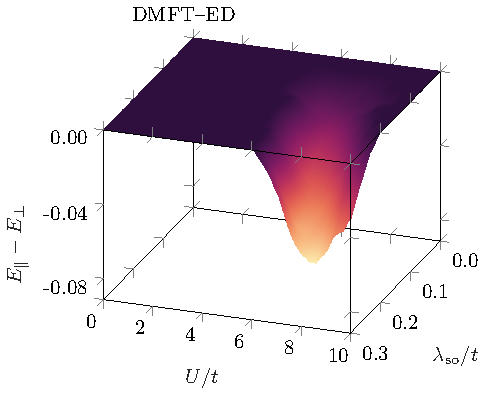
\includegraphics[width=0.47\linewidth,trim={0 0 0 5mm},clip]{figures/KMH_energy.pdf}\hfill
    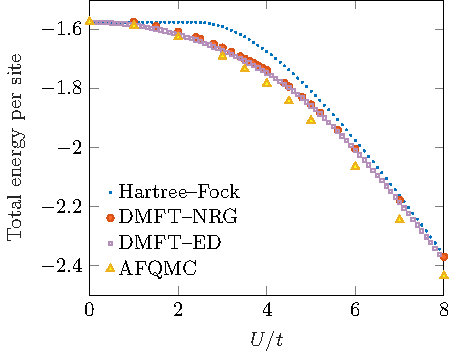
\includegraphics[width=0.45\linewidth]{figures/benchEnergy_honey.pdf}\\
    \caption{In panel (a) we report the total energy difference between 
    the in-plane and the
    off-plane AFM solutions found with \NAME at $T=0$. Negative values
    signal a ground state with in-plane magnetization. The plateau at zero
    energy difference marks the topological phase of the model (a 
    paramagnetic quantum spin-Hall insulator), at all points except on the $\lambda_\mathrm{so}=0$ line, where the ground state is an interacting
    Dirac liquid, at weak coupling, or an isotropic antiferromagnet at strong coupling. In panel (b) we compare the total energies, across the 
    $\lambda_\mathrm{so}=0$ line, to published data for Hartree-Fock,
    DMFT-NRG and AFQMC solutions \cite{Raczkowski2020PRB}.}
    \label{fig:KMenergy}
\end{figure}






\begin{figure}
    \centering
    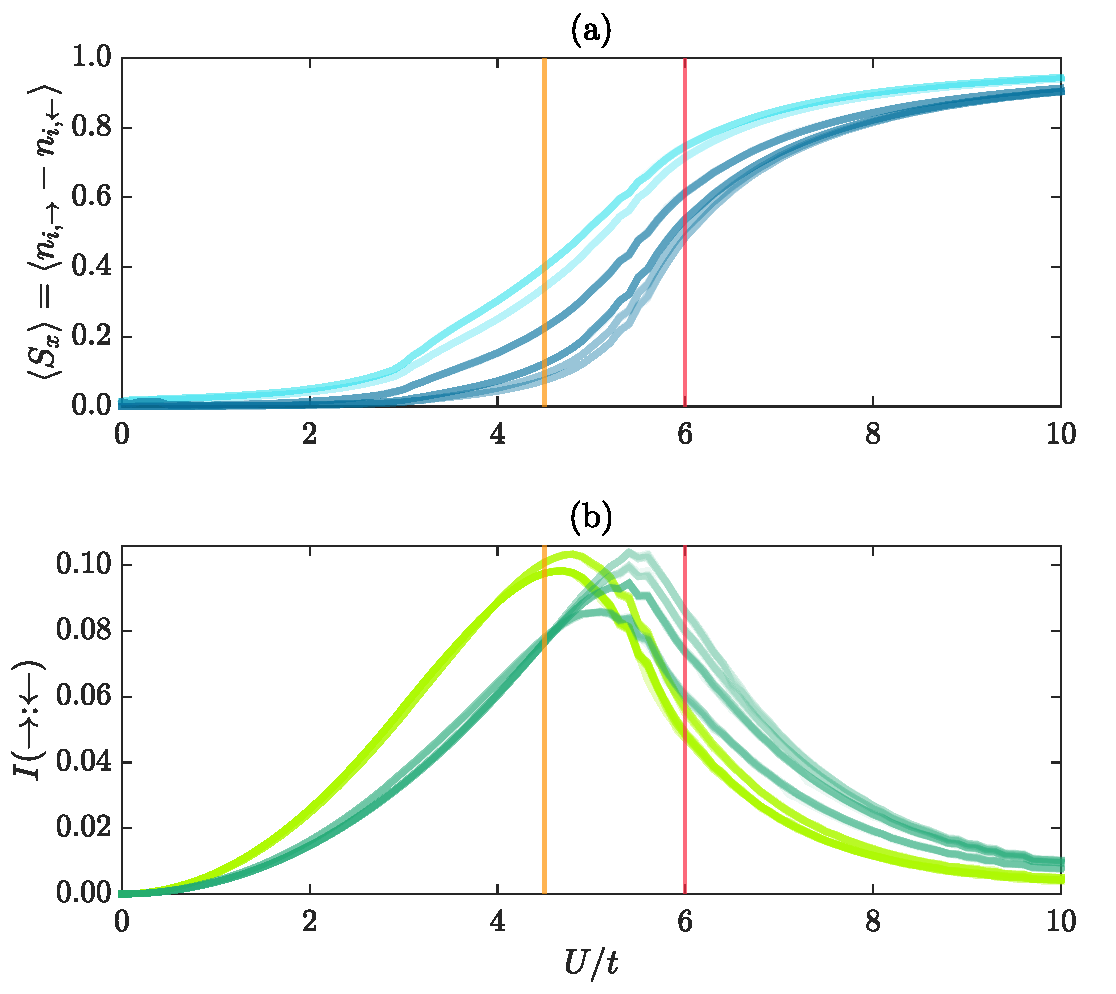
\includegraphics[width=0.8\linewidth]{figures/flakes_edipack.pdf}\\[1mm]
    (c) \hspace{10cm} (d) \\
    \hspace{1.2cm}
    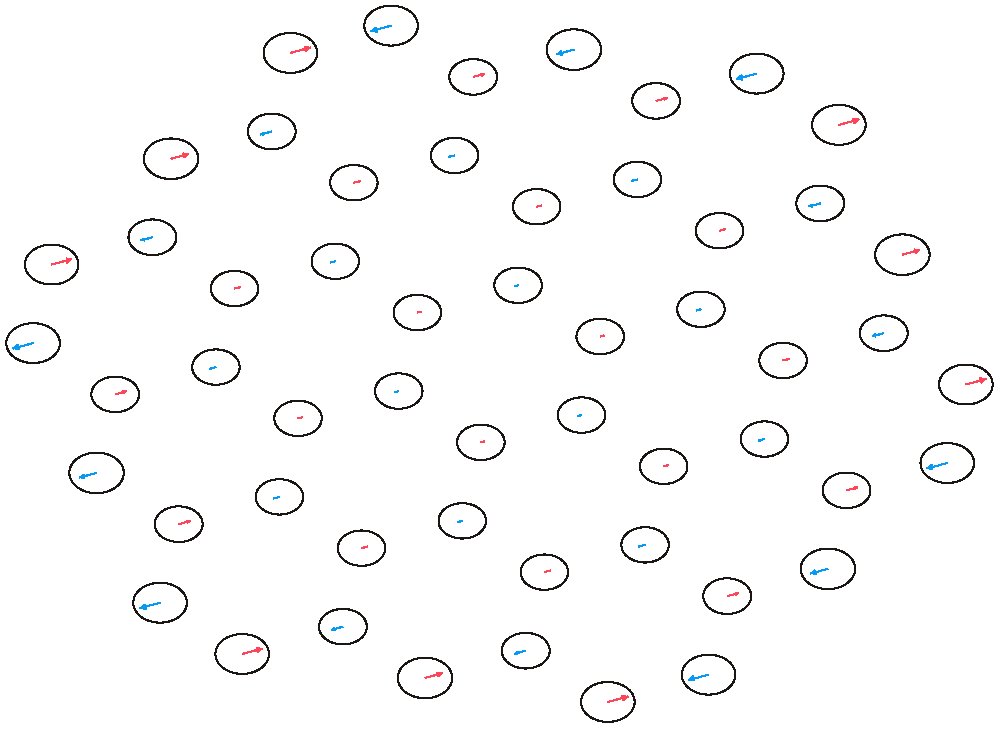
\includegraphics[width=0.33\linewidth]{figures/3NflakeU4.5_x.pdf} \hspace{1.2cm}
    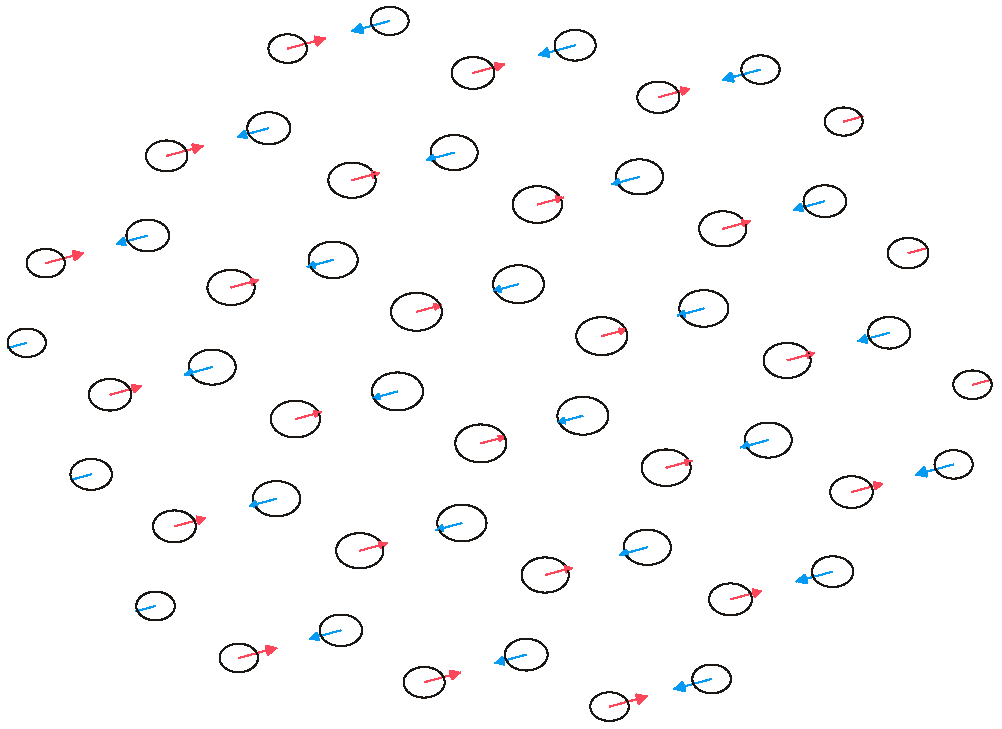
\includegraphics[width=0.33\linewidth]{figures/3NflakeU6_x.pdf} \vspace{3mm}
    \caption{Kane-Mele-Hubbard model at the nanoscale.
    In (a) the local in-plane
    magnetization $\ibra S_x \iket = \ibra n_{i,\rightarrow}-n_{i,\leftarrow}\iket$. In
    (b) the local correlation as measured by the mutual 
    information between local in-plane spin eigenstates
    $I(\rightarrow:\leftarrow)$ \cite{BellomiaPhD,BellomiaKMH,Bellomia_intracorr}. 
    Both the (a) and (b) panels mark the edge and ``bulk'' 
    sites in lighter and darker colors, respectively.
    In (c) and (d) a visual representation of the given 
    nano-system at different values of $U/t$, as marked 
    respectively by the orange and red vertical lines 
    in panels (a) and (b). The area of the 
    circles is proportional to $I(\rightarrow:\leftarrow)$, 
    the length of the arrows to $\ibra S_x \iket$.
    All data are taken at $\lambda_\mathrm{so}=0.3t$ and $T=0$.}
    \label{fig:KMflake}
\end{figure}


\subsubsection{Kane-Mele-Hubbard model at the nanoscale}
The capabilities of the EDIpack2ineq layer go well beyond the
simple case of a two-site unit cell. Building on the previous example, we can readily adapt the calculation to deal with a nanoscopic \cite{Amaricci2014PRA} system with $N_\mathrm{ineq}$ inequivalent atoms, such as hexagonal flakes
\cite{Valli2016PRB,Valli2018NL}.
We consider a 
$N_\mathrm{ineq}\times N_\mathrm{ineq}$ local Hamiltonian 
$H_\mathrm{loc}$ with open boundary conditions, and implementing
the self-consistent equations with a trivial single momentum 
$k=0$. In this configuration the system develops an inhomogeneous magnetization, so that in general no particular lattice symmetry group, e.g. N\'eel, can be exploited. 
% Some lowered point symmetry can be found, but a 
% safer approach of solving all the $N_\mathrm{ineq}$ impurity models
% leads to good results, with fair control of spatial numerical noise.

In \figu{fig:KMflake} we report results for a nanosystem of 
$N_\mathrm{ineq}=54$ sites, solved with the bath parametrization 
described in \equ{eq:afmx_dmft_ansatz}, for the in-plane 
antiferromagnetic state.
Panel (a) shows the interaction dependence of the local magnetization,
computed from the impurity ground state as  
$ \ibra S_x \iket = \ibra c^\dagger_{i,\up} c_{i,\dw} + c^\dagger_{i,\dw} c_{i,\up} \iket \equiv \ibra n_{i,\rightarrow} \iket - \ibra n_{i,\leftarrow} \iket$,
so that we can define the $S_x$ spin occupation numbers as
\begin{equation*}
    \ibra n_{i,\rightarrow} \iket \equiv \frac{\ibra n_{i,\up} + n_{i,\dw} \iket +
    \ibra c^\dagger_{i,\up} c_{i,\dw} + c^\dagger_{i,\dw} c_{i,\up} \iket}{2},
    \qquad
    \ibra n_{i,\leftarrow} \iket \equiv \frac{\ibra n_{i,\up} + n_{i,\dw} \iket -
    \ibra c^\dagger_{i,\up} c_{i,\dw} + c^\dagger_{i,\dw} c_{i,\up} \iket}{2},
\end{equation*}
which trivially satisfy the conservation of the local average charge $\ibra n_{i,\rightarrow} + n_{i,\leftarrow} \iket = \ibra n_{i,\up} + n_{i,\dw} \iket$.
Having a direct expression for $\ibra n_{i,\rightarrow} \iket$ and $\ibra n_{i,\leftarrow} \iket$
we can verify that the impurity reduced density matrix, computed by 
tracing the bath states in the \texttt{ed\_mode=nonsu2} representation 
(see \ref{sSecRDM}), once diagonalized, takes the familiar form
\cite{Zanardi2002PRA,Su2013MPLB,Walsh2019PRL} 
\begin{equation}
    \rho^\mathrm{imp} = 
     \begin{pmatrix}
            \left\ibra\left(1-n_{i,\rightarrow}\right)\left(1-n_{i,\leftarrow}\right)\right\iket   &    0          &       0       &   0 \\
                    0       &    \left\ibra n_{i,\rightarrow}\left(1-n_{i,\leftarrow}\right)\right\iket  &       0       &   0 \\
                   0       &       0   &    \left\ibra\left(1-n_{i,\rightarrow}\right)n_{i,\leftarrow}\right\iket      &   0 \\
                    0       &       0   &       0          &    \left\ibra n_{i,\rightarrow} n_{i,\leftarrow}\right\iket
        \end{pmatrix} 
\end{equation}
in the basis of the {\it natural} spin-orbitals
\cite{BellomiaPhD,BellomiaKMH,Bellomia_intracorr}, 
whose occupation numbers
are given by $n_{i,\rightarrow}$ and $n_{i,\leftarrow}$.
As  discussed in \cite{BellomiaPhD,BellomiaKMH,Bellomia_intracorr},
by defining the spin traces of $\rho^\mathrm{imp}$, as
\begin{equation}
    \rho^\mathrm{imp}_\sigma = 
    \Tr_{\bar{\sigma}} \left[\rho^\mathrm{imp}\right] =
    \begin{pmatrix}
        \ibra n_{i,\sigma} \iket & 0 \\
        0 & \ibra n_{i,\bar{\sigma}} \iket
    \end{pmatrix}
\end{equation}
we can directly measure local correlations by defining the mutual information
between the impurity spin-orbitals
$I(\rightarrow:\leftarrow) = 
    S(\rho^\mathrm{imp}_{\rightarrow}) + 
    S(\rho^\mathrm{imp}_{\leftarrow}) -
    S(\rho^\mathrm{imp})$,
where $S(\cdot)$ denotes the von Neumann entropy of its argument.

In panel (b) of \figu{fig:KMflake} we report the spatially resolved
interaction dependency of $I(\rightarrow:\leftarrow)$, as a direct 
observation of the enhanced local correlations at the boundary of the
finite system. While it is usually assumed that edge sites must be
more correlated than internal (``bulk'') sites, based on the reduced
lattice coordination, the inter-spin mutual information quantifies directly the phenomenon: the edge correlations,
marked in lighter green, are decidedly higher as long as the system 
remains in a weakly magnetized regime. When the local magnetization
exceeds half of its saturation value, all local correlations start to decrease,
as spin fluctuations are damped by ordering. Significantly, the edge 
correlations get lower than the bulk correlations as the maximum is 
crossed, consistently with the observation that their magnetization
is always higher and so their fluctuations are frozen faster.
Finally, we observe that the nanosystem of \figu{fig:KMflake} has 
finite local magnetization for arbitrary low interaction strengths,
in striking contrast with the infinite lattice. This is a well-known
effect of quantum confinement, as proposed in early works on graphene
flakes \cite{Valli2016PRB,Valli2018NL}.



%% References with bibTeX database:
\ifSubfilesClassLoaded{
  \bibliography{references}
}{}
\end{document}



%%%%%%%%%%%%%%%%%%%%%%%%%%%%%%%%%%%%%%%%%%%%%%%%%%%%%%%%%%%%%%%%%%
%%%%%%%%%%%%%%%%%%%%%%%%%%%%%%%%%%%%%%%%%%%%%%%%%%%%%%%%%%%%%%%%%%
%%%%%%%%%%%%%%%%%%%%%%%%%%%%%%%%%%%%%%%%%%%%%%%%%%%%%%%%%%%%%%%%%%
%%%%%%%%%%%%%%%%%%%%%%%%%%%%%%%%%%%%%%%%%%%%%%%%%%%%%%%%%%%%%%%%%%


\section{Conclusions}

%%%%%%%%%%%%%%%%%%%%%%%%%%%%%%%%%%%%%%%%%%%%%%%%%%%%%%%%%%%%%%%%%%
%%%%%%%%%%%%%%%%%%%%%%%%%%%%%%%%%%%%%%%%%%%%%%%%%%%%%%%%%%%%%%%%%%
%%%%%%%%%%%%%%%%%%%%%%%%%%%%%%%%%%%%%%%%%%%%%%%%%%%%%%%%%%%%%%%%%%
%%%%%%%%%%%%%%%%%%%%%%%%%%%%%%%%%%%%%%%%%%%%%%%%%%%%%%%%%%%%%%%%%%

\section*{Acknowledgements}

\section{Appendix A: Monicelli interface}


%% References with bibTeX database:
% \section*{References}
\bibliographystyle{elsarticle-num}
\bibliography{references}






\end{document}








